% ---------------------------------------------------------------------------------------------------------------
% Appendix (draft, 14 Nov 2026). % ---------------------------------------------------------------------------------------------------------------
% Appendix (draft, 14 Nov 2026). % ---------------------------------------------------------------------------------------------------------------
% Appendix (draft, 14 Nov 2026). % ---------------------------------------------------------------------------------------------------------------
% Appendix (draft, 14 Nov 2026). \input{appendix.tex} after the main text and before the bibliography.
% Needs in the preamble: \usepackage{booktabs,makecell,rotating} (algorithm2e, amsmath, graphicx are already loaded).
% Every table is generated: latex/tables/*.tex by analysis/paper_tables.py (the tables moved out of Section 4),
% latex/tables/appendix/*.tex by analysis/appendix_tables.py; nothing in a table is typed.
% Labels used by the main text: app:A6 (recruit size), app:A17 (rank mobility), alg:period (Section 3.3).
% Suggested split if the journal's printed length is tight: A and B printed, C and D as an online supplement.
% ---------------------------------------------------------------------------------------------------------------
\appendix
\numberwithin{table}{section}
\numberwithin{figure}{section}
\renewcommand{\thetable}{\thesection\arabic{table}}
\renewcommand{\thefigure}{\thesection\arabic{figure}}

\section{Model details and benchmarks}\label{app:model}

\subsection{Order of events within a period}\label{app:algorithm}

Algorithm~\ref{alg:period} gives the order of events within a period. Merger and exit decisions use the window $\{t-l, \dots, t-1\}$; the current period's shock is never part of the information on which a decision is taken, and a unit formed in period $t$ pools from period $t$ on.

\begin{algorithm}[H]
\caption{Order of events within a period}\label{alg:period}
\SetAlgoLined
Draw $x_{it}$ for all firms; compute $G_{mt}$ and $\tilde r_{it}$\;
[endogenous-$\alpha$ block] every unit renegotiates $\alpha_C$ on the grid over the last $l$ periods: unanimity first, maximin second\;
\ForEach{firm $i$ drawn as initiator with probability $p$}{
  draw a target market among those its unit does not occupy and a target firm in it\;
  \If{the merged set has at most one firm per market and $\tilde\Delta_i(\hat C, \alpha) > \max\{0, \tilde\Delta_i(C_i, \alpha)\}$ for every member}{
    merge; set the entry period of every new member (of every member if two units merge) to $t$\;
  }
}
\ForEach{conglomerate}{
  $\delta_{jt}$ for each member by the pooling equation; a member whose factor would fall below zero keeps nothing and its shortfall is charged to the other members pro rata to their post-pooling capital\;
}
$s_{i,t+1} = s_{it}\,\delta_{it}$ for members, $s_{it}\,e^{\tilde r_{it}}$ for unaffiliated firms\;
\ForEach{market}{
  lift every firm below $c \times$ mean size to that level, iterating to the fixed point; count floor hits; a lifted member leaves its unit; renormalize the market to mean size one\;
}
\ForEach{member with tenure $> l$}{
  leave if $\tilde\Delta_i(C_i, \alpha) < 0$\;
}
dissolve units with one member\;
every 100 periods: record the size distribution, membership and unit capital\;
\end{algorithm}

Two details of the floor. Since sizes are shares of a market whose capital is the numeraire, an entrant's share dilutes the incumbents' shares in proportion to their size, as any entry does; after pooling and the floor every market is renormalized to mean size one, which is where this dilution takes place. What survives the loss of the firm's capital is the configuration's knowledge, whether as the same firm recapitalized or as a start-up formed by its people, and with it its record.

\subsection{The equal-members reference}\label{app:kstar}

$K^*$ is the scope that maximizes the time-average growth of a member in a unit of equal members facing i.i.d.\ shocks at the median market volatility $q = 0.20$, net of the coordination cost. It is computed by Monte Carlo ($2 \times 10^6$ draws per $K$) and capped at $M = 50$. Table~\ref{tab:a1_kstar} gives it for every family and cost form at the three reference sharing rates; Table~\ref{tab:a1b_kstar_cost} for the higher cost levels of the power-law form. The reference rises with the sharing rate and with tail weight, and under $t_3$ shocks it reaches the cap at every cost form but the quadratic. Section~\ref{sec:decision} explains why it is a reference and not a prediction: the gain from a recruit depends on the capital weights the members actually have, which the equal-members calculation does not see.

\input{tables/appendix/a1_kstar.tex}
\input{tables/appendix/a1b_kstar_cost.tex}

\subsection{Floor calibration}\label{app:floor}

The floor $c$ is set in the unaffiliated Laplace economy ($\alpha = 0$) so that the median Hill exponent of the top decile of within-market shares equals 1.06 \citep{axtell2001zipf}. Table~\ref{tab:a2_floor_calibration} is the calibration grid: for each $N$ and $c$ the Hill exponent (median and interquartile range over runs), the within-market Herfindahl index and the share of firms at the floor, from runs with $M = 20$ and $T = 8{,}000$. The column $1/(1-c)$ is the exponent of the continuous-time reflected process; the exponent of the simulated economy with finitely many firms per market differs from it in both directions, which is why $c$ is calibrated on the simulated economy and not set from the formula. The interpolated value at $N = 50$ is $c^* = 0.12717$; at $N = 25$ it is 0.069 and at $N = 100$ it is 0.158, which is what the economy-size block uses. The calibration is to the light-tailed families: at $c^*$ the normal and Laplace economies give 1.07 and 1.06, $t_3$ 1.00 and $\nu = 2.5$ 0.96.

\input{tables/appendix/a2_floor_calibration.tex}

\subsection{Burn-in}\label{app:burnin}

Twenty runs (Laplace at $\alpha \in \{0, 0.1, 0.3\}$, $t_3$ at $\alpha = 0.3$, five seeds each, the main-block scenarios) were extended from $T = 11{,}000$ to $T = 16{,}000$ under the moment rule; every run reproduces its main-block result to period 11,000 exactly. Table~\ref{tab:a3_burnin} compares the means of scope, pooled capital share, floor-hit rates by status and the Hill exponent over periods 11,000--16,000 with their means over the retained window 8,000--11,000. The difference is the mean over seeds of each run's own later-minus-pilot difference, in per cent of its pilot-window mean; the last column is a 95\% confidence interval ($\pm 1.96$ standard errors across the five seeds) for that mean difference. The interval is read against the pre-registered 2\% tolerance, not against the point estimate: an estimate near zero inside an interval of $\pm 1$--$1.5$ points is what the absence of drift looks like, and every interval lies inside the tolerance. The seventeen means are all within 0.54\%; an OLS trend of the $t_3$ pooled share over the extended run is $+0.02\%$ per 1,000 periods ($p = 0.57$); scope and pooled share reach their long-run level within the first 600 periods. The same check under the loggain rule gives 0.71\%.

\input{tables/appendix/a3_burnin.tex}

\subsection{Simulation design}\label{app:design}

Table~\ref{tab:design} lists the blocks of the design described in Section~\ref{sec:calibration}; every block holds every parameter at its main-block value except the one it varies.

\begin{table}[htbp]
\centering
\caption{Simulation design}
\label{tab:design}
\small
\begin{tabular}{lp{0.36\linewidth}p{0.12\linewidth}p{0.17\linewidth}r}
\toprule
Block & What varies & Families & $\alpha$ & Runs \\
\midrule
main & --; all four cost schedules & all three & grid & 540 \\
\addlinespace[3pt]
\multicolumn{5}{l}{\emph{Environment}} \\
$\nu$ & Student-$t$ with $\nu \in \{2.5, 4\}$ & $t$ & 0.1, 0.3, 0.5 & 30 \\
correlation & $\rho = 0.3$ (Gaussian copula) & Laplace & grid & 45 \\
floor level & $c \in \{0.10, 0.35\}$ & Laplace & grid & 90 \\
size & $(M, N) \in \{25, 100\}^2$ with $c^*(N)$ & Laplace & 0, 0.1, 0.3, 0.5 & 80 \\
homogeneous & every market at $q = 0.20$; moment and loggain rules & all three & 0.05, 0.1, 0.3, 0.5 & 120 \\
\addlinespace[3pt]
\multicolumn{5}{l}{\emph{Contract}} \\
equal split & net pool split equally; all four cost schedules & normal & grid & 180 \\
cost level & $\times 0.5$, $\times 2$: all four schedules (linear and quadratic also with $b_1, b_2$ scaled); $\times 5$, $\times 10$, $\times 20$: power law & Laplace; $t_3$ at the high levels & grid; 0.1, 0.3, 0.5 at the high levels & 630 \\
endogenous $\alpha$ & $\alpha_C$ renegotiated by each unit, start 0.1; all four cost schedules & all three & -- & 60 \\
$\alpha$ beyond the grid & the main power-law scenarios at $\alpha \in \{0.6, 0.7, 0.8, 0.9\}$ & all three & 0.6--0.9 & 60 \\
\addlinespace[3pt]
\multicolumn{5}{l}{\emph{Decisions}} \\
lookback & $l \in \{20, 50, 100, 200, 500\}$ & Laplace, $t_3$ & 0.1, 0.3 & 100 \\
search & $p \in \{0.2, 1\}$ & all three & 0.05, 0.1, 0.3, 0.5 & 120 \\
\addlinespace[3pt]
\multicolumn{5}{l}{\emph{Rule controls (3.3)}} \\
cv & exact replay minus its first-order term & all three & 0.1, 0.3, 0.5 & 45 \\
accept & every feasible proposal accepted, no voluntary exit & all three & 0.1, 0.3, 0.5 & 45 \\
\midrule
total &  &  &  & 2,145 \\
\bottomrule
\end{tabular}
\par\smallskip\begin{minipage}{0.95\linewidth}\footnotesize Five replications per cell; ``grid'' is the nine-value $\alpha$ grid of the main block; power-law cost unless stated. Every cell of the original design except the $\nu$ block is also run under the loggain rule with the same seeds (2,100 runs; appendix).\end{minipage}
\end{table}

\section{Additional results}\label{app:results}

\subsection{Scope and turnover in full}\label{app:scope}

Tables~\ref{tab:scope} and \ref{tab:turnover} give the main-block cells behind Figure~\ref{fig:scope}, Table~\ref{tab:scope} with the $\alpha = 0.7$ and $0.9$ cells added (the main scenarios rerun at $\alpha = 0.6$--$0.8$, and the fixed $\alpha = 0.9$ cell): scope under the moment rule and its loggain twin, the equal-members reference, the pooled capital share and the acceptance rate; floor and voluntary exits per period and the floor-hit rate by status. Table~\ref{tab:window} gives scope by window length, which Figure~\ref{fig:search}(c) plots, and Table~\ref{tab:a4_loggain_main} the full main block under the loggain rule. The effective number of members, the inverse Herfindahl of members' capital weights, is 0.68--0.70 of $K$ at $\alpha = 0.3$ (Table~\ref{tab:a18_concentration}): the typical unit is a few partners of unequal size rather than an equal-weighted pool.

\input{tables/table3_scope.tex}
\input{tables/table3t_turnover.tex}
\input{tables/table3b_window.tex}
\input{tables/appendix/a4_loggain_main.tex}

\subsection{Consent by scope and recruit size}\label{app:A6}

Table~\ref{tab:a5_acceptance_by_K} is the data of Figure~\ref{fig:consent}: the acceptance rate of feasible proposals by the size $K$ of the prospective unit at $\alpha = 0.3$ and $p = 0.05$, under both rules, with the median estimated gain of the binding member (the member with the smallest margin, $\tilde\Delta_i(\hat C) - \max\{0, \tilde\Delta_i(C_i)\}$), the equal-weight marginal gain of the $K$-th member and the marginal coordination cost. Acceptance falls monotonically in $K$ under both rules and the binding gain crosses zero at $K = 5$--6 under the moment rule and at $K = 4$ under loggain, well before the marginal cost catches up with the equal-weight gain.

Table~\ref{tab:a6_recruit_size} splits the same proposals by the size of the recruit. A floor recruit is a standalone entrant with a market share below $2c/N$; the incumbent margin is the exact second-order gain of an incumbent from an entrant of the observed mean weight, net of the marginal cost. Floor recruits are 45--81\% of proposals at $K \leq 10$, and the incumbents' margin on them turns negative at $K = 7$--10. The proposals with an entrant weight of 0.2 or more are not explained by recruit size; Table~\ref{tab:a6b_unit_unit} shows that these are unit--unit mergers (42--46\% of that group at $K = 4$, 88--100\% at $K \geq 8$) and that it is the more volatile side that refuses: when the entrant unit is the calmer one, the volatile incumbent unit holds the binding member in two-thirds to seven-eighths of the proposals and acceptance is about half that of the opposite case. This is the direction of the transfer term in the gain: pooling gross factors moves arithmetic growth from members above the unit's average variance to those below it. Under $t_3$ the mean binding gain of floor recruits is set by rare large estimates and stays positive while acceptance falls; the counters hold mean and standard deviation only.

\input{tables/appendix/a5_acceptance_by_K.tex}
\input{tables/appendix/a6_recruit_size.tex}
\input{tables/appendix/a6b_unit_unit.tex}

\subsection{The decision rule: approximation and an exact control}\label{app:rule}

The moment rule is a second-order expansion of the replayed log growth of the window. Table~\ref{tab:a7_approximation} measures what it omits on 27 traced runs with 2,000 random decision points each (a standalone firm and $K - 1$ standalone partners from other markets, $\tilde\Delta$ and the replay $\hat\Delta$ on the same 50-period window). The omitted higher-order terms, computed with the capital weights frozen at the window's first period, are 1--2\% of the gain at the median. The 20--38\% median difference between the two rules is almost entirely the replay's first-order term, the term with expectation zero whose in-window realization makes the replay biased low in finite windows.

The cv rule averages the exact replayed log gain minus that first-order term, so it is exact in expectation and expands nothing. Table~\ref{tab:a7b_cv_statistic} compares the three statistics on the same windows: the cv statistic differs from the moment statistic by 1--2\% at the median and changes the sign of the decision in about 0.1\% of draws or fewer, where loggain changes it in 0.7--2.3\%. Table~\ref{tab:a7c_cv_behaviour} runs the cv rule on the main power-law cells (45 runs on the main cells' seeds): it reproduces the moment rule to within 0.11 members, 0.005 in pooled share and 0.03 in the Hill exponent, with acceptance by $K$ within 0.02 at every $K \leq 12$. The second-order approximation therefore has no effect on any outcome reported in the paper; the loggain rule's smaller scope is the finite-window bias and noise of the replay's first-order term, which is what Section~\ref{sec:results-scope} calls verifiability.

\input{tables/appendix/a7_approximation.tex}
\input{tables/appendix/a7b_cv_statistic.tex}
\input{tables/appendix/a7c_cv_behaviour.tex}

\subsection{Owners' growth and survival}\label{app:owners}

Table~\ref{tab:owner-byK} splits the owner-return gap of Table~\ref{tab:owner} by the size of the member's unit and Table~\ref{tab:hazard} gives the floor-hit rates by status from which its hazard ratio is formed; both are from the 27 traced runs, means over three replications. The gap is largest in the largest units in every cell.

\input{tables/table4a_owner_by_K.tex}
\input{tables/table4b_hazard.tex}

\paragraph*{Growth after entry.}\label{app:eventstudy}
An event study was run alongside the status panel. For each firm that joins a unit at $t$, a control is a standalone in the same market, unaffiliated over the 50 preceding periods, with the closest log share at $t$ (within 0.25); the post-entry gap is the joiner's owner-path growth minus the control's over the 50 periods after entry, net of recapitalization at the floor. The post-entry gap is positive in every family $\times$ $\alpha$ cell (0.01--0.26 percentage points per period, rising with $\alpha$) under every matching tried. The difference in differences is not reported as a result: firms in a market are identical ex ante but not ex post, and the one ex-post variable that can be matched, size at entry, selects controls with a different recapitalization history (a standalone at the joiner's size tends to be one just lifted by the floor), so the pre-entry paths differ and the sign of the before--after comparison follows the matching. Table~\ref{tab:a14_event_study} keeps the four matchings as the record of that check; the owner-return result in the main text rests on the status panel, which compares all member-periods with all standalone-periods within market and size decile and needs no matching.

\input{tables/appendix/a14_event_study.tex}

\subsection{Clustering of floor hits}\label{app:burstiness}

Table~\ref{tab:a15_burstiness} is the data of Figure~\ref{fig:burstiness}: the index of dispersion of floor hits per market-period against its binomial reference, the share of market-periods with three or more hits, and the worst market-period in a run; means over three traced replications. Floor hits cluster in every family (index 2.4--4.6 against a binomial 0.9), most under $t_3$, and pooling reduces the clustering without removing it.

\input{tables/appendix/a15_burstiness.tex}

\subsection{Growth-rate distributions of members and standalones}\label{app:growth}

Per-period log growth of market share before any floor lift, market-demeaned and divided by the market's shock IQR, over all post-burn-in firm-periods of the 27 traced runs, by status (Table~\ref{tab:a16_growth_status}) and by unit size (Table~\ref{tab:a16b_growth_by_K}); Figure~\ref{fig:growth_density} shows the densities at $\alpha = 0.3$ on a log axis with maximum-likelihood Laplace fits. Three findings. Shape: members' growth rates stay in their family; under Laplace shocks MAD/SD is 0.71--0.72 (Laplace 0.707) and the Laplace fit beats the normal by 0.05--0.06 nats per observation, as for standalones; the normal family stays normal; $t_3$ members are pulled slightly towards Laplace but stay heavier-tailed. Scale: at $\alpha = 0.3$ the members' standard deviation is 0.77 of the standalones' (0.87 at $K = 2$, 0.81 at $K = 3$--4, 0.76 at $K \geq 5$), within 0.005 of what linear pooling of gross returns with the units' actual capital weights predicts. Tails: the lower tail is cut more than the scale (first-percentile ratio 0.71 under Laplace against a standard-deviation ratio of 0.77) and the upper tail less (99th-percentile ratio 0.82), so members' growth is right-skewed (+0.28) where standalones' is symmetric: a large own loss is floored by the partners' share while a large own gain passes through. This compression of the lower tail is the mechanism behind the tail-exponent result of Section~\ref{sec:results-distribution}. The model has no size--volatility relation for standalones by construction (the standard deviation is flat across size deciles); members show a mild rising one (decile 10 over decile 1, 1.03--1.10), as the weights predict, because a large member is a large part of its own unit.

\input{tables/appendix/a16_growth_status.tex}
\input{tables/appendix/a16b_growth_by_K.tex}

\begin{figure}[htbp]
\centering
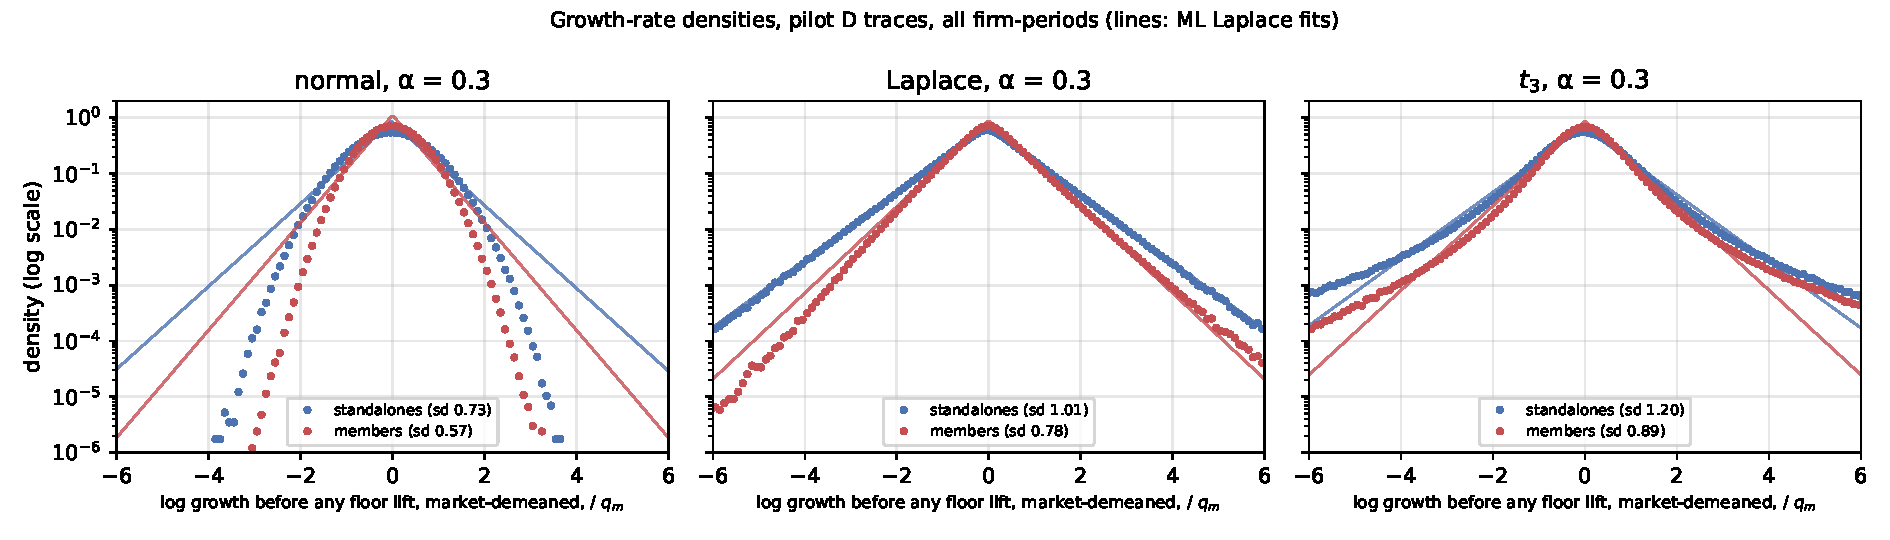
\includegraphics[width=\linewidth]{figures/appendix/growth_density_alpha0.3.pdf}
\caption{Densities of normalized per-period growth rates of members and standalones at $\alpha = 0.3$, log axis, with maximum-likelihood Laplace fits; one panel per family. 27 traced runs, moment rule.}
\label{fig:growth_density}
\end{figure}

\subsection{Concentration and rank mobility}\label{app:A17}

Table~\ref{tab:a18_concentration} gives the concentration measures behind Section~\ref{sec:results-distribution}. Within markets firms become more equal: the within-market Herfindahl index falls from 0.175--0.20 at $\alpha = 0$ to 0.14--0.17 at $\alpha = 0.3$ and 0.11--0.14 at $\alpha = 0.5$. Across the economy the units that own them become fewer and larger: the capital held by the largest ten per cent of owners, a conglomerate counted as one owner, goes from 0.65 to 0.65 (normal, with 0.67 at $\alpha = 0.3$), 0.66 to 0.74 (Laplace) and 0.68 to 0.79 ($t_3$) between $\alpha = 0$ and $0.5$; beyond $0.5$ it falls to 0.53 (normal) and 0.67 (Laplace) at $\alpha = 0.9$ while $t_3$ reaches 0.81, as the units' members grow more equal in size ($K_{\text{eff}}/K$ rises again to 0.68--0.71). Units sort by volatility and grow unequal: assortativity, the dispersion of members' market volatilities relative to that of a random set of the same size, falls from 0.60--0.61 at $\alpha = 0.01$ to 0.35--0.36 at $\alpha = 0.5$, because the consent test selects partners whose fluctuations are worth sharing from both sides; the effective number of members falls from 0.83--0.88 of $K$ to 0.64--0.68 over the same range as units accumulate a few large members and many recruits from the floor.

Tables~\ref{tab:a17_rank_mobility} and \ref{tab:a17b_rank_mobility_status} measure rank mobility from the 27 traced runs and nine traced $\alpha = 0$ runs: within each market, ranks of log share at an origin every 100 periods and 100 periods later, giving the Spearman correlation, the persistence of the top and bottom decile, leader turnover and the mean absolute rank change; a hit-free sample drops firms lifted at the floor in between and re-ranks the rest; the same by status at the origin; and the same for owning units across the economy. Pooling lowers rank mobility within markets in every family (lag-100 Spearman 0.16--0.33 at $\alpha = 0$ against 0.25--0.45 at $\alpha = 0.3$; top-decile persistence 0.31--0.48 against 0.36--0.53), partly through fewer floor lifts (0.68--0.83 of firms lifted within 100 periods against 0.52--0.71) and partly through slower movement among going concerns (members' ranks move 9--20\% less than standalones'); and it makes the top decile of owners markedly more persistent (0.32--0.49 against 0.67--0.69). Mobility is high in every cell and ranks are nearly independent at lag 500. The per-firm rank range and rank standard deviation of the earlier draft, recomputed on the traces, are at their ceiling in the floored economy and move the same way.

\input{tables/appendix/a18_concentration.tex}
\input{tables/appendix/a17_rank_mobility.tex}
\input{tables/appendix/a17b_rank_mobility_status.tex}

\subsection{Scope without consent: the accept rule}\label{app:accept}

Under the accept rule every feasible proposal merges and no one leaves by choice; everything else is unchanged. It is a control without knowledge, not a behavioural alternative: it shows the scope the floor and the one-firm-per-market constraint alone permit. Table~\ref{tab:a19_accept} sets it beside the moment and loggain rules on the main power-law cells (45 runs on the main cells' seeds): $K_{\text{accept}}$ is 12.4--28.2 against 3.5--7.7, above the equal-members reference in every normal and Laplace cell and below it under $t_3$ (0.3--0.6 of $K^*$). The extra mergers are solo entries of floor-sized firms into existing units (86--89\% of the control's entries are at the floor); unit--unit mergers do not rise with consent off, because consolidated units occupy most markets and clash. The pooled share rises by 0.02--0.11, the Hill exponent by 0.00--0.04, the within-market Herfindahl index falls by 0.004--0.012, and the members' floor-hit rate rises slightly. Table~\ref{tab:decomposition-accept} is the four-part re-cut of Table~\ref{tab:decomposition} that separates what the environment permits from what consent withholds.

\input{tables/appendix/a19_accept.tex}
\input{tables/table3c_decomposition_accept.tex}

\subsection{The sharing rate}\label{app:alpha}

Table~\ref{tab:endogenous} gives the endogenous-$\alpha$ block under the power-law cost and Table~\ref{tab:a13_endogenous} under all four cost forms and both rules. Units that choose their rate reach 14--18 mean members under the power-law cost, with 95--98\% of capital pooled and a tail exponent of 1.8--2.1. This is the scope that a rate near 0.9 implies, not a separate effect: along the fixed-rate grid $K$ rises from 5.4 at $\alpha = 0.3$ to 7.8 at $0.5$, and the fixed $\alpha = 0.9$ cell reproduces the endogenous block (Table~\ref{tab:robustness-b}). The ordering across families is the same as elsewhere: the heaviest tails choose a slightly lower rate and reach a smaller scope. The exponential-cost cells reach $K = 16$--23 at a lower pooled share (81--92\%). Neither heterogeneity among members nor the volatility of their markets drives the choice: across 7,630 units active at the end of a run, the Spearman correlation of a unit's time-averaged rate with the dispersion of its members' volatilities is $-0.14$ to $0.00$, and with their mean volatility 0.04--0.10. Under the loggain rule the latter was 0.14--0.26: units in more volatile markets pooled more, not because the optimum differed, it is full pooling at every volatility level, but because only there was the gain from a higher rate large enough to show through the window's noise.

\input{tables/table5_endogenous_alpha.tex}
\input{tables/appendix/a13_endogenous.tex}

\section{Robustness}\label{app:robustness}

\subsection{Summary}

Tables~\ref{tab:robustness} and \ref{tab:robustness-b} summarize every block at $\alpha = 0.3$ (the endogenous-$\alpha$ block at its adopted rate) against the Laplace power-law baseline. The rest of this section gives each block in full.

\input{tables/table6_robustness.tex}
\input{tables/table6c_robustness_contract.tex}

\subsection{Cost form and level}\label{app:cost}

Table~\ref{tab:a10_cost_forms} gives the four cost forms at equal $\Phi(40)$ for all three families; the form moves scope by under one member. Table~\ref{tab:costlevel} runs the power-law level from $\times 0.5$ to $\times 20$ at $\alpha = 0.3$ under both rules with the equal-members reference recomputed at each level: scope falls by about 0.6 members per doubling of the cost and the ratio $K/K^*$ rises, but the reference is never reached, because the reference falls with the cost as well. Table~\ref{tab:a10b_cost_levels} gives the $\times 0.5$ and $\times 2$ cells for every form, with $b_0$ alone scaled (power law and exponential: the whole schedule) or all coefficients scaled (linear, quadratic).

\input{tables/appendix/a10_cost_forms.tex}
\input{tables/table6b_cost_level.tex}
\input{tables/appendix/a10b_cost_levels.tex}

\subsection{Floor level, correlation and economy size}\label{app:environment}

Tables~\ref{tab:a11a_floor}--\ref{tab:a11c_size}, Laplace shocks and power-law cost. The floor level sets the tail exponent and little else: scope moves by $+3\%$ at $c = 0.10$ and $-19\%$ at $c = 0.35$ while the Hill exponent moves from 1.13 to 1.66 at $\alpha = 0.3$. Cross-market correlation of 0.3 leaves every outcome within 0.2 of the baseline. Economy size matters through the number of firms per market and barely through the number of markets, with the floor recalibrated to $c^*(N)$.

\input{tables/appendix/a11a_floor.tex}
\input{tables/appendix/a11b_correlation.tex}
\input{tables/appendix/a11c_size.tex}

\subsection{Homogeneous markets}\label{app:homogeneous}

Table~\ref{tab:a8_homogeneous}: every market at $q = 0.20$, power-law cost, both rules. The homogeneous economy is the $K_{\text{hom}}$ of Table~\ref{tab:decomposition}; it exceeds the heterogeneous base case by 0.0--0.4 members, which bounds the transfer conflict between members of unequal volatility.

\input{tables/appendix/a8_homogeneous.tex}

\subsection{Tail weight}\label{app:nu}

Table~\ref{tab:a9_nu}: Student-$t$ shocks with $\nu \in \{2.5, 3, 4\}$ at equal IQR, power-law cost, moment rule. The last two columns give the distribution of the window variance estimate relative to its population value over 200,000 i.i.d.\ 50-period windows at $q = 0.2$, and the share of windows in which it is below one half. Scope falls with tail weight while acceptance rises: under heavier tails firms are more willing to pool and less able to stay pooled, because members are recapitalized more often. Attrition, not consent, takes the scope.

\input{tables/appendix/a9_nu.tex}

\subsection{Equal sharing}\label{app:equalsplit}

Table~\ref{tab:a12_equal_split}: equal dollar splits of the net pool, normal shocks, four cost forms, with acceptance by proposal type (standalone--standalone, standalone--unit), voluntary exits, pool ruin (a unit's members capped at limited liability in a period) and the shortfall charged to the other members. Mean scope is 2.1--3.2 at every sharing rate and pooled capital never exceeds 34\%, against 3.2--7.7 and up to 96\% under proportional sharing. The reason is visible in who consents: proposals between two unaffiliated firms pass at 3--48\% under equal sharing against 95--100\% under proportional, proposals of a standalone to a unit at 6--17\% against 28--41\%. Under an equal split the larger partner subsidizes the smaller in every period in which it does better, which it expects to do half the time, and refuses. The contract decides whether conglomerates exist at all.

\input{tables/appendix/a12_equal_split.tex}

\section{Computation}\label{app:computation}

\subsection{Identity protocol and tests}\label{app:identity}

Every change to the code after the model was frozen (the diagnostics, the limited-liability correction, the counters, the moment rule, the production block and the traced runs) was accompanied by an identity check: every scenario whose behaviour the change should not touch is rerun on the new code and its result and summary row compared byte for byte with the stored ones, excluding runtime fields and new keys. The production block passes 1,995 of 1,995 scenarios and the accept-rule addition 2,055 of 2,055; the loggain reference block is frozen and verified by checksum. The test suite (281 tests) covers the pooling identity under limited liability (unit capital after pooling equals the sum of members' gross returns net of the coordination cost, to $10^{-9}$), the moment rule against hand-computed cases and against the loggain replay on long windows, the kernel counters' sums, the design counts and the summary schema. Three pool wipeouts (every member of a unit at the floor in the same period) occurred in 1,995 runs, one event each; they are counted, not asserted away.

\subsection{Files and provenance}\label{app:files}

The repository holds the simulation code, the design files, the per-run summaries of the production block and the loggain reference block, the traced runs' panels and every derived file behind a table or figure; \texttt{analysis/paper\_tables.py}, \texttt{analysis/paper\_figures.py} and \texttt{analysis/appendix\_tables.py} regenerate every exhibit from them. The commit the paper is frozen on and the archive DOI are given in the code and data availability statement.
 after the main text and before the bibliography.
% Needs in the preamble: \usepackage{booktabs,makecell,rotating} (algorithm2e, amsmath, graphicx are already loaded).
% Every table is generated: latex/tables/*.tex by analysis/paper_tables.py (the tables moved out of Section 4),
% latex/tables/appendix/*.tex by analysis/appendix_tables.py; nothing in a table is typed.
% Labels used by the main text: app:A6 (recruit size), app:A17 (rank mobility), alg:period (Section 3.3).
% Suggested split if the journal's printed length is tight: A and B printed, C and D as an online supplement.
% ---------------------------------------------------------------------------------------------------------------
\appendix
\numberwithin{table}{section}
\numberwithin{figure}{section}
\renewcommand{\thetable}{\thesection\arabic{table}}
\renewcommand{\thefigure}{\thesection\arabic{figure}}

\section{Model details and benchmarks}\label{app:model}

\subsection{Order of events within a period}\label{app:algorithm}

Algorithm~\ref{alg:period} gives the order of events within a period. Merger and exit decisions use the window $\{t-l, \dots, t-1\}$; the current period's shock is never part of the information on which a decision is taken, and a unit formed in period $t$ pools from period $t$ on.

\begin{algorithm}[H]
\caption{Order of events within a period}\label{alg:period}
\SetAlgoLined
Draw $x_{it}$ for all firms; compute $G_{mt}$ and $\tilde r_{it}$\;
[endogenous-$\alpha$ block] every unit renegotiates $\alpha_C$ on the grid over the last $l$ periods: unanimity first, maximin second\;
\ForEach{firm $i$ drawn as initiator with probability $p$}{
  draw a target market among those its unit does not occupy and a target firm in it\;
  \If{the merged set has at most one firm per market and $\tilde\Delta_i(\hat C, \alpha) > \max\{0, \tilde\Delta_i(C_i, \alpha)\}$ for every member}{
    merge; set the entry period of every new member (of every member if two units merge) to $t$\;
  }
}
\ForEach{conglomerate}{
  $\delta_{jt}$ for each member by the pooling equation; a member whose factor would fall below zero keeps nothing and its shortfall is charged to the other members pro rata to their post-pooling capital\;
}
$s_{i,t+1} = s_{it}\,\delta_{it}$ for members, $s_{it}\,e^{\tilde r_{it}}$ for unaffiliated firms\;
\ForEach{market}{
  lift every firm below $c \times$ mean size to that level, iterating to the fixed point; count floor hits; a lifted member leaves its unit; renormalize the market to mean size one\;
}
\ForEach{member with tenure $> l$}{
  leave if $\tilde\Delta_i(C_i, \alpha) < 0$\;
}
dissolve units with one member\;
every 100 periods: record the size distribution, membership and unit capital\;
\end{algorithm}

Two details of the floor. Since sizes are shares of a market whose capital is the numeraire, an entrant's share dilutes the incumbents' shares in proportion to their size, as any entry does; after pooling and the floor every market is renormalized to mean size one, which is where this dilution takes place. What survives the loss of the firm's capital is the configuration's knowledge, whether as the same firm recapitalized or as a start-up formed by its people, and with it its record.

\subsection{The equal-members reference}\label{app:kstar}

$K^*$ is the scope that maximizes the time-average growth of a member in a unit of equal members facing i.i.d.\ shocks at the median market volatility $q = 0.20$, net of the coordination cost. It is computed by Monte Carlo ($2 \times 10^6$ draws per $K$) and capped at $M = 50$. Table~\ref{tab:a1_kstar} gives it for every family and cost form at the three reference sharing rates; Table~\ref{tab:a1b_kstar_cost} for the higher cost levels of the power-law form. The reference rises with the sharing rate and with tail weight, and under $t_3$ shocks it reaches the cap at every cost form but the quadratic. Section~\ref{sec:decision} explains why it is a reference and not a prediction: the gain from a recruit depends on the capital weights the members actually have, which the equal-members calculation does not see.

\begin{table}[htbp]
\centering
\caption{Planner's optimum $K^*$ by family, cost form and $\alpha$}
\label{tab:a1_kstar}
\small
\begin{tabular}{lrrrr}
\toprule
Family & Cost form & $\alpha$ = 0.1 & 0.3 & 0.5 \\
\midrule
normal & power law & 8 & 12 & 13 \\
normal & linear & 7 & 12 & 13 \\
normal & quadratic & 10 & 13 & 16 \\
normal & exponential & 12 & 18 & 22 \\
Laplace & power law & 10 & 16 & 20 \\
Laplace & linear & 10 & 16 & 20 \\
Laplace & quadratic & 12 & 17 & 20 \\
Laplace & exponential & 15 & 22 & 29 \\
$t_3$ & power law & 20 & 47 & 50 \\
$t_3$ & linear & 28 & 47 & 50 \\
$t_3$ & quadratic & 24 & 29 & 38 \\
$t_3$ & exponential & 47 & 50 & 50 \\
\bottomrule
\end{tabular}
\end{table}

\begin{table}[htbp]
\centering
\caption{$K^*$ at higher cost levels (power law)}
\label{tab:a1b_kstar_cost}
\small
\begin{tabular}{lrrrr}
\toprule
Family & Cost level & $\alpha$ = 0.1 & 0.3 & 0.5 \\
\midrule
Laplace & $\times$5 & 5 & 8 & 9 \\
Laplace & $\times$10 & 4 & 6 & 7 \\
Laplace & $\times$20 & 3 & 4 & 5 \\
$t_3$ & $\times$5 & 7 & 10 & 13 \\
$t_3$ & $\times$10 & 4 & 7 & 9 \\
$t_3$ & $\times$20 & 3 & 5 & 6 \\
\bottomrule
\end{tabular}
\end{table}


\subsection{Floor calibration}\label{app:floor}

The floor $c$ is set in the unaffiliated Laplace economy ($\alpha = 0$) so that the median Hill exponent of the top decile of within-market shares equals 1.06 \citep{axtell2001zipf}. Table~\ref{tab:a2_floor_calibration} is the calibration grid: for each $N$ and $c$ the Hill exponent (median and interquartile range over runs), the within-market Herfindahl index and the share of firms at the floor, from runs with $M = 20$ and $T = 8{,}000$. The column $1/(1-c)$ is the exponent of the continuous-time reflected process; the exponent of the simulated economy with finitely many firms per market differs from it in both directions, which is why $c$ is calibrated on the simulated economy and not set from the formula. The interpolated value at $N = 50$ is $c^* = 0.12717$; at $N = 25$ it is 0.069 and at $N = 100$ it is 0.158, which is what the economy-size block uses. The calibration is to the light-tailed families: at $c^*$ the normal and Laplace economies give 1.07 and 1.06, $t_3$ 1.00 and $\nu = 2.5$ 0.96.

\begin{table}[htbp]
\centering
\caption{Floor calibration grid}
\label{tab:a2_floor_calibration}
\small
\begin{tabular}{lrrrrr}
\toprule
N & c & 1/(1 $-$ c) & Hill [IQR] & HHI within & share at floor \\
\midrule
25 & 0.0300 & 1.031 & 0.927 [0.913, 0.951] & 0.329 & 0.074 \\
25 & 0.0500 & 1.053 & 1.006 [0.986, 1.028] & 0.280 & 0.087 \\
25 & 0.0566 & 1.060 & 1.026 [1.017, 1.043] & 0.266 & 0.081 \\
25 & 0.0800 & 1.087 & 1.090 [1.072, 1.107] & 0.232 & 0.089 \\
25 & 0.1000 & 1.111 & 1.144 [1.129, 1.160] & 0.211 & 0.100 \\
25 & 0.1270 & 1.145 & 1.221 [1.209, 1.233] & 0.187 & 0.109 \\
25 & 0.1500 & 1.176 & 1.261 [1.249, 1.294] & 0.170 & 0.112 \\
25 & 0.2000 & 1.250 & 1.354 [1.340, 1.374] & 0.143 & 0.122 \\
25 & 0.3000 & 1.429 & 1.590 [1.562, 1.600] & 0.105 & 0.154 \\
50 & 0.0300 & 1.031 & 0.798 [0.797, 0.804] & 0.263 & 0.087 \\
50 & 0.0500 & 1.053 & 0.865 [0.839, 0.872] & 0.222 & 0.092 \\
50 & 0.0566 & 1.060 & 0.900 [0.874, 0.903] & 0.216 & 0.091 \\
50 & 0.0800 & 1.087 & 0.960 [0.942, 0.962] & 0.183 & 0.099 \\
50 & 0.1000 & 1.111 & 1.006 [0.998, 1.009] & 0.155 & 0.103 \\
50 & 0.1500 & 1.176 & 1.106 [1.088, 1.114] & 0.119 & 0.125 \\
50 & 0.2000 & 1.250 & 1.197 [1.192, 1.208] & 0.097 & 0.129 \\
50 & 0.3000 & 1.429 & 1.392 [1.385, 1.429] & 0.067 & 0.167 \\
50 & 0.4000 & 1.667 & 1.616 [1.616, 1.626] & 0.049 & 0.193 \\
50 & 0.5000 & 2.000 & 1.862 [1.818, 1.869] & 0.037 & 0.237 \\
100 & 0.0800 & 1.087 & 0.909 [0.906, 0.923] & 0.139 & 0.103 \\
100 & 0.1000 & 1.111 & 0.950 [0.943, 0.951] & 0.125 & 0.113 \\
100 & 0.1270 & 1.145 & 0.992 [0.990, 1.012] & 0.103 & 0.114 \\
100 & 0.1500 & 1.176 & 1.044 [1.043, 1.049] & 0.089 & 0.135 \\
100 & 0.2000 & 1.250 & 1.141 [1.125, 1.161] & 0.068 & 0.140 \\
100 & 0.3000 & 1.429 & 1.347 [1.311, 1.363] & 0.042 & 0.166 \\
200 & 0.0566 & 1.060 & 0.833 [0.832, 0.842] & 0.138 & 0.115 \\
200 & 0.1500 & 1.176 & 1.035 [1.030, 1.035] & 0.063 & 0.139 \\
200 & 0.3000 & 1.429 & 1.303 [1.298, 1.307] & 0.029 & 0.176 \\
\bottomrule
\end{tabular}
\end{table}


\subsection{Burn-in}\label{app:burnin}

Twenty runs (Laplace at $\alpha \in \{0, 0.1, 0.3\}$, $t_3$ at $\alpha = 0.3$, five seeds each, the main-block scenarios) were extended from $T = 11{,}000$ to $T = 16{,}000$ under the moment rule; every run reproduces its main-block result to period 11,000 exactly. Table~\ref{tab:a3_burnin} compares the means of scope, pooled capital share, floor-hit rates by status and the Hill exponent over periods 11,000--16,000 with their means over the retained window 8,000--11,000. The difference is the mean over seeds of each run's own later-minus-pilot difference, in per cent of its pilot-window mean; the last column is a 95\% confidence interval ($\pm 1.96$ standard errors across the five seeds) for that mean difference. The interval is read against the pre-registered 2\% tolerance, not against the point estimate: an estimate near zero inside an interval of $\pm 1$--$1.5$ points is what the absence of drift looks like, and every interval lies inside the tolerance. The seventeen means are all within 0.54\%; an OLS trend of the $t_3$ pooled share over the extended run is $+0.02\%$ per 1,000 periods ($p = 0.57$); scope and pooled share reach their long-run level within the first 600 periods. The same check under the loggain rule gives 0.71\%.

\begin{sidewaystable}[htbp]
\centering
\caption{Burn-in check: later window against the pilot window}
\label{tab:a3_burnin}
\small
\begin{tabular}{lrrrrrr}
\toprule
Family & $\alpha$ & Series & \makecell[b]{Pilot\\{}window} & \makecell[b]{Periods\\{}11,000--16,000} & \makecell[b]{Difference,\\{}\% of pilot mean} & \makecell[b]{95\% CI,\\{}$\pm$ \% points} \\
\midrule
Laplace & 0 & Floor-hit rate, standalone (all-firm) & 0.1151 & 0.1152 & +0.09\% & $\pm$1.05 \\
Laplace & 0 & Hill exponent & 1.0710 & 1.0653 & -0.52\% & $\pm$1.54 \\
Laplace & 0.1 & Mean K & 3.7061 & 3.6973 & -0.24\% & $\pm$0.34 \\
Laplace & 0.1 & Pooled capital share & 0.8521 & 0.8529 & +0.10\% & $\pm$1.00 \\
Laplace & 0.1 & Floor-hit rate, standalone (all-firm) & 0.0865 & 0.0865 & +0.05\% & $\pm$1.11 \\
Laplace & 0.1 & Floor-hit rate, member (all-firm) & 0.0193 & 0.0193 & +0.15\% & $\pm$1.21 \\
Laplace & 0.1 & Hill exponent & 1.1037 & 1.0978 & -0.52\% & $\pm$1.47 \\
Laplace & 0.3 & Mean K & 5.3869 & 5.3722 & -0.27\% & $\pm$0.43 \\
Laplace & 0.3 & Pooled capital share & 0.9146 & 0.9135 & -0.12\% & $\pm$0.17 \\
Laplace & 0.3 & Floor-hit rate, standalone (all-firm) & 0.0697 & 0.0696 & +0.04\% & $\pm$1.41 \\
Laplace & 0.3 & Floor-hit rate, member (all-firm) & 0.0148 & 0.0148 & +0.22\% & $\pm$1.48 \\
Laplace & 0.3 & Hill exponent & 1.1994 & 1.1960 & -0.27\% & $\pm$1.00 \\
$t_3$ & 0.3 & Mean K & 4.8312 & 4.8258 & -0.11\% & $\pm$0.77 \\
$t_3$ & 0.3 & Pooled capital share & 0.8927 & 0.8944 & +0.18\% & $\pm$0.41 \\
$t_3$ & 0.3 & Floor-hit rate, standalone (all-firm) & 0.0821 & 0.0816 & -0.50\% & $\pm$0.86 \\
$t_3$ & 0.3 & Floor-hit rate, member (all-firm) & 0.0175 & 0.0175 & -0.45\% & $\pm$0.67 \\
$t_3$ & 0.3 & Hill exponent & 1.1169 & 1.1168 & +0.00\% & $\pm$1.24 \\
\bottomrule
\end{tabular}
\par\smallskip\begin{minipage}{0.95\linewidth}\footnotesize Means over replications of each run's window means; difference in per cent of the pilot-window mean; CI across the five seeds.\end{minipage}
\end{sidewaystable}


\subsection{Simulation design}\label{app:design}

Table~\ref{tab:design} lists the blocks of the design described in Section~\ref{sec:calibration}; every block holds every parameter at its main-block value except the one it varies.

\begin{table}[htbp]
\centering
\caption{Simulation design}
\label{tab:design}
\small
\begin{tabular}{lp{0.36\linewidth}p{0.12\linewidth}p{0.17\linewidth}r}
\toprule
Block & What varies & Families & $\alpha$ & Runs \\
\midrule
main & --; all four cost schedules & all three & grid & 540 \\
\addlinespace[3pt]
\multicolumn{5}{l}{\emph{Environment}} \\
$\nu$ & Student-$t$ with $\nu \in \{2.5, 4\}$ & $t$ & 0.1, 0.3, 0.5 & 30 \\
correlation & $\rho = 0.3$ (Gaussian copula) & Laplace & grid & 45 \\
floor level & $c \in \{0.10, 0.35\}$ & Laplace & grid & 90 \\
size & $(M, N) \in \{25, 100\}^2$ with $c^*(N)$ & Laplace & 0, 0.1, 0.3, 0.5 & 80 \\
homogeneous & every market at $q = 0.20$; moment and loggain rules & all three & 0.05, 0.1, 0.3, 0.5 & 120 \\
\addlinespace[3pt]
\multicolumn{5}{l}{\emph{Contract}} \\
equal split & net pool split equally; all four cost schedules & normal & grid & 180 \\
cost level & $\times 0.5$, $\times 2$: all four schedules (linear and quadratic also with $b_1, b_2$ scaled); $\times 5$, $\times 10$, $\times 20$: power law & Laplace; $t_3$ at the high levels & grid; 0.1, 0.3, 0.5 at the high levels & 630 \\
endogenous $\alpha$ & $\alpha_C$ renegotiated by each unit, start 0.1; all four cost schedules & all three & -- & 60 \\
$\alpha$ beyond the grid & the main power-law scenarios at $\alpha \in \{0.6, 0.7, 0.8, 0.9\}$ & all three & 0.6--0.9 & 60 \\
\addlinespace[3pt]
\multicolumn{5}{l}{\emph{Decisions}} \\
lookback & $l \in \{20, 50, 100, 200, 500\}$ & Laplace, $t_3$ & 0.1, 0.3 & 100 \\
search & $p \in \{0.2, 1\}$ & all three & 0.05, 0.1, 0.3, 0.5 & 120 \\
\addlinespace[3pt]
\multicolumn{5}{l}{\emph{Rule controls (3.3)}} \\
cv & exact replay minus its first-order term & all three & 0.1, 0.3, 0.5 & 45 \\
accept & every feasible proposal accepted, no voluntary exit & all three & 0.1, 0.3, 0.5 & 45 \\
\midrule
total &  &  &  & 2,145 \\
\bottomrule
\end{tabular}
\par\smallskip\begin{minipage}{0.95\linewidth}\footnotesize Five replications per cell; ``grid'' is the nine-value $\alpha$ grid of the main block; power-law cost unless stated. Every cell of the original design except the $\nu$ block is also run under the loggain rule with the same seeds (2,100 runs; appendix).\end{minipage}
\end{table}

\section{Additional results}\label{app:results}

\subsection{Scope and turnover in full}\label{app:scope}

Tables~\ref{tab:scope} and \ref{tab:turnover} give the main-block cells behind Figure~\ref{fig:scope}, Table~\ref{tab:scope} with the $\alpha = 0.7$ and $0.9$ cells added (the main scenarios rerun at $\alpha = 0.6$--$0.8$, and the fixed $\alpha = 0.9$ cell): scope under the moment rule and its loggain twin, the equal-members reference, the pooled capital share and the acceptance rate; floor and voluntary exits per period and the floor-hit rate by status. Table~\ref{tab:window} gives scope by window length, which Figure~\ref{fig:search}(c) plots, and Table~\ref{tab:a4_loggain_main} the full main block under the loggain rule. The effective number of members, the inverse Herfindahl of members' capital weights, is 0.68--0.70 of $K$ at $\alpha = 0.3$ (Table~\ref{tab:a18_concentration}): the typical unit is a few partners of unequal size rather than an equal-weighted pool.

\begin{table}[htbp]
\centering
\caption{Scope; main block, power-law cost; medians over five replications}
\label{tab:scope}
\small
\begin{tabular}{lrrrrrrr}
\toprule
Family & $\alpha$ & $K$ & $K$, loggain & $K^*$ & $K/K^*$ & Pooled & Accept. \\
\midrule
normal & 0.05 & 3.2 & 2.7 & -- & -- & 0.76 & 0.32 \\
 & 0.1 & 3.7 & 3.0 & 8 & 0.46 & 0.85 & 0.31 \\
 & 0.3 & 5.5 & 4.3 & 12 & 0.46 & 0.94 & 0.29 \\
 & 0.5 & 7.7 & 6.3 & 13 & 0.59 & 0.96 & 0.27 \\
\midrule
Laplace & 0.05 & 3.2 & 2.7 & -- & -- & 0.78 & 0.43 \\
 & 0.1 & 3.7 & 3.0 & 10 & 0.37 & 0.85 & 0.43 \\
 & 0.3 & 5.4 & 4.0 & 16 & 0.34 & 0.91 & 0.40 \\
 & 0.5 & 7.8 & 5.9 & 20 & 0.39 & 0.93 & 0.38 \\
\midrule
$t_3$ & 0.05 & 3.1 & 2.7 & -- & -- & 0.76 & 0.47 \\
 & 0.1 & 3.5 & 2.9 & 20 & 0.17 & 0.83 & 0.47 \\
 & 0.3 & 4.8 & 3.7 & 47 & 0.10 & 0.90 & 0.44 \\
 & 0.5 & 6.8 & 5.1 & 50 & 0.14 & 0.92 & 0.41 \\
\bottomrule
\end{tabular}
\par\smallskip\begin{minipage}{0.95\linewidth}\footnotesize $K$: mean members per active unit (moment rule; loggain twin from pilot C); $K^*$: equal-members reference at the median market volatility, capped at $M = 50$; pooled: share of economy capital held by members; acceptance: share of feasible proposals accepted.\end{minipage}
\end{table}

\begin{table}[htbp]
\centering
\caption{Turnover and floor hits; main block, power-law cost; medians over five replications}
\label{tab:turnover}
\small
\begin{tabular}{lrrrrr}
\toprule
Family & $\alpha$ & Floor exits & Vol.\ exits & Member hits & Standalone hits \\
\midrule
normal & 0.05 & 36.1 & 0.19 & 0.024 & 0.178 \\
 & 0.1 & 34.1 & 0.06 & 0.021 & 0.185 \\
 & 0.3 & 25.0 & 0.00 & 0.014 & 0.187 \\
 & 0.5 & 15.6 & 0.00 & 0.008 & 0.178 \\
 & 0.7 & 7.6 & 0.00 & 0.004 & 0.165 \\
 & 0.9 & 2.4 & 0.00 & 0.001 & 0.136 \\
\midrule
Laplace & 0.05 & 49.4 & 0.09 & 0.037 & 0.201 \\
 & 0.1 & 47.4 & 0.02 & 0.034 & 0.207 \\
 & 0.3 & 36.3 & 0.00 & 0.022 & 0.211 \\
 & 0.5 & 24.5 & 0.00 & 0.014 & 0.206 \\
 & 0.7 & 12.9 & 0.00 & 0.006 & 0.197 \\
 & 0.9 & 4.9 & 0.00 & 0.002 & 0.175 \\
\midrule
$t_3$ & 0.05 & 55.0 & 0.10 & 0.044 & 0.207 \\
 & 0.1 & 53.1 & 0.04 & 0.041 & 0.212 \\
 & 0.3 & 42.5 & 0.00 & 0.028 & 0.218 \\
 & 0.5 & 31.2 & 0.00 & 0.019 & 0.219 \\
 & 0.7 & 19.7 & 0.00 & 0.011 & 0.216 \\
 & 0.9 & 10.5 & 0.00 & 0.005 & 0.202 \\
\bottomrule
\end{tabular}
\par\smallskip\begin{minipage}{0.95\linewidth}\footnotesize Exits per period among 2,500 firms (mergers per period equal floor exits to within 0.2); member / standalone hits: floor hits per firm-period of that status.\end{minipage}
\end{table}

\begin{table}[htbp]
\centering
\caption{Window length, power-law cost; medians over five replications}
\label{tab:window}
\small
\begin{tabular}{lrrrrrr}
\toprule
Family & $\alpha$ & $l = 20$ & 50 & 100 & 200 & 500 \\
\midrule
Laplace, $K$ & 0.1 & 3.4 / 2.7 & 3.7 / 3.0 & 3.9 / 3.2 & 4.1 / 3.5 & 4.6 / 3.9 \\
Laplace, $K$ & 0.3 & 4.8 / 3.3 & 5.4 / 4.0 & 5.8 / 4.4 & 6.1 / 4.8 & 6.6 / 5.4 \\
$t_3$, $K$ & 0.1 & 3.2 / 2.6 & 3.5 / 2.9 & 3.7 / 3.1 & 3.8 / 3.3 & 4.1 / 3.7 \\
$t_3$, $K$ & 0.3 & 4.3 / 3.0 & 4.9 / 3.7 & 5.2 / 4.1 & 5.2 / 4.3 & 5.4 / 4.9 \\
\bottomrule
\end{tabular}
\par\smallskip\begin{minipage}{0.95\linewidth}\footnotesize Cells: moment / loggain. Floor exits per period do not depend on $l$ (35--38 under Laplace, 41--47 under $t_3$ at $\alpha = 0.3$); voluntary exits are nil at every $l$ under the moment rule and fall from about five per period at $l = 20$ to none beyond $l = 200$ under loggain.\end{minipage}
\end{table}

\begin{table}[htbp]
\centering
\caption{Main block under the loggain rule}
\label{tab:a4_loggain_main}
\small
\begin{tabular}{lrrrrrrr}
\toprule
Family & $\alpha$ & K & Pooled & Hill & Accept. & \makecell[b]{Voluntary\\{}exits / period} & \makecell[b]{Floor\\{}exits / period} \\
\midrule
normal & 0.05 & 2.7 & 0.47 & 1.08 & 0.33 & 3.6 & 36.0 \\
normal & 0.1 & 3.0 & 0.56 & 1.09 & 0.33 & 3.0 & 34.8 \\
normal & 0.3 & 4.3 & 0.73 & 1.17 & 0.28 & 1.4 & 26.0 \\
normal & 0.5 & 6.3 & 0.91 & 1.32 & 0.23 & 0.2 & 16.1 \\
Laplace & 0.05 & 2.7 & 0.56 & 1.07 & 0.42 & 2.0 & 48.1 \\
Laplace & 0.1 & 3.0 & 0.63 & 1.10 & 0.41 & 1.8 & 46.8 \\
Laplace & 0.3 & 4.0 & 0.78 & 1.16 & 0.36 & 0.9 & 36.9 \\
Laplace & 0.5 & 5.9 & 0.91 & 1.33 & 0.32 & 0.2 & 25.1 \\
$t_3$ & 0.05 & 2.7 & 0.56 & 1.00 & 0.46 & 1.7 & 53.3 \\
$t_3$ & 0.1 & 2.9 & 0.63 & 1.02 & 0.45 & 1.6 & 52.1 \\
$t_3$ & 0.3 & 3.7 & 0.77 & 1.10 & 0.40 & 0.9 & 43.2 \\
$t_3$ & 0.5 & 5.1 & 0.88 & 1.18 & 0.36 & 0.3 & 32.3 \\
\bottomrule
\end{tabular}
\end{table}


\subsection{Consent by scope and recruit size}\label{app:A6}

Table~\ref{tab:a5_acceptance_by_K} is the data of Figure~\ref{fig:consent}: the acceptance rate of feasible proposals by the size $K$ of the prospective unit at $\alpha = 0.3$ and $p = 0.05$, under both rules, with the median estimated gain of the binding member (the member with the smallest margin, $\tilde\Delta_i(\hat C) - \max\{0, \tilde\Delta_i(C_i)\}$), the equal-weight marginal gain of the $K$-th member and the marginal coordination cost. Acceptance falls monotonically in $K$ under both rules and the binding gain crosses zero at $K = 5$--6 under the moment rule and at $K = 4$ under loggain, well before the marginal cost catches up with the equal-weight gain.

Table~\ref{tab:a6_recruit_size} splits the same proposals by the size of the recruit. A floor recruit is a standalone entrant with a market share below $2c/N$; the incumbent margin is the exact second-order gain of an incumbent from an entrant of the observed mean weight, net of the marginal cost. Floor recruits are 45--81\% of proposals at $K \leq 10$, and the incumbents' margin on them turns negative at $K = 7$--10. The proposals with an entrant weight of 0.2 or more are not explained by recruit size; Table~\ref{tab:a6b_unit_unit} shows that these are unit--unit mergers (42--46\% of that group at $K = 4$, 88--100\% at $K \geq 8$) and that it is the more volatile side that refuses: when the entrant unit is the calmer one, the volatile incumbent unit holds the binding member in two-thirds to seven-eighths of the proposals and acceptance is about half that of the opposite case. This is the direction of the transfer term in the gain: pooling gross factors moves arithmetic growth from members above the unit's average variance to those below it. Under $t_3$ the mean binding gain of floor recruits is set by rare large estimates and stays positive while acceptance falls; the counters hold mean and standard deviation only.

\begin{sidewaystable}[htbp]
\centering
\caption{Acceptance and binding gain by K, both rules}
\label{tab:a5_acceptance_by_K}
\small
\begin{tabular}{lrrrrrrr}
\toprule
Family & K & \makecell[b]{Acceptance,\\{}moment} & loggain & \makecell[b]{Binding median,\\{}moment} & loggain & \makecell[b]{Marginal\\{}gain} & \makecell[b]{Marginal\\{}cost} \\
\midrule
normal & 2 & 1.00 & 0.92 & 2.7e-03 & 1.7e-03 & 2.8e-03 & 2.6e-05 \\
 & 3 & 0.90 & 0.55 & 5.6e-04 & 5.8e-05 & 9.3e-04 & 2.9e-05 \\
 & 4 & 0.67 & 0.38 & 1.2e-04 & -6.9e-05 & 4.7e-04 & 3.1e-05 \\
 & 5 & 0.48 & 0.28 & -4.7e-06 & -9.8e-05 & 2.8e-04 & 3.3e-05 \\
 & 6 & 0.35 & 0.21 & -3.3e-05 & -1.1e-04 & 1.9e-04 & 3.4e-05 \\
 & 7 & 0.27 & 0.17 & -4.4e-05 & -1.2e-04 & 1.3e-04 & 3.5e-05 \\
 & 8 & 0.20 & 0.14 & -5.4e-05 & -1.5e-04 & 1.0e-04 & 3.6e-05 \\
 & 9 & 0.16 & 0.10 & -6.5e-05 & -1.9e-04 & 7.8e-05 & 3.7e-05 \\
 & 10 & 0.12 & 0.07 & -8.2e-05 & -2.9e-04 & 6.2e-05 & 3.8e-05 \\
 & 11 & 0.08 & 0.05 & -1.3e-04 & -4.3e-04 & 5.1e-05 & 3.9e-05 \\
 & 12 & 0.04 & 0.03 & -2.8e-04 & -5.7e-04 & 4.2e-05 & 4.0e-05 \\
Laplace & 2 & 1.00 & 0.97 & 5.2e-03 & 3.6e-03 & 5.7e-03 & 2.6e-05 \\
 & 3 & 0.87 & 0.59 & 9.9e-04 & 1.8e-04 & 1.9e-03 & 2.9e-05 \\
 & 4 & 0.69 & 0.41 & 2.3e-04 & -8.1e-05 & 9.5e-04 & 3.1e-05 \\
 & 5 & 0.54 & 0.31 & 3.0e-05 & -1.4e-04 & 5.7e-04 & 3.3e-05 \\
 & 6 & 0.44 & 0.25 & -2.4e-05 & -1.7e-04 & 3.8e-04 & 3.4e-05 \\
 & 7 & 0.37 & 0.21 & -4.4e-05 & -1.9e-04 & 2.7e-04 & 3.5e-05 \\
 & 8 & 0.31 & 0.17 & -5.5e-05 & -1.9e-04 & 2.0e-04 & 3.6e-05 \\
 & 9 & 0.25 & 0.14 & -6.5e-05 & -2.5e-04 & 1.6e-04 & 3.7e-05 \\
 & 10 & 0.21 & 0.11 & -7.6e-05 & -3.4e-04 & 1.3e-04 & 3.8e-05 \\
 & 11 & 0.17 & 0.09 & -9.4e-05 & -5.4e-04 & 1.0e-04 & 3.9e-05 \\
 & 12 & 0.13 & 0.07 & -1.4e-04 & -7.3e-04 & 8.6e-05 & 4.0e-05 \\
$t_3$ & 2 & 1.00 & 0.97 & 5.8e-03 & 4.1e-03 & 6.1e-03 & 2.6e-05 \\
 & 3 & 0.76 & 0.57 & 8.1e-04 & 1.5e-04 & 2.0e-03 & 2.9e-05 \\
 & 4 & 0.59 & 0.39 & 1.2e-04 & -1.3e-04 & 1.0e-03 & 3.1e-05 \\
 & 5 & 0.48 & 0.30 & -1.5e-05 & -2.0e-04 & 6.1e-04 & 3.3e-05 \\
 & 6 & 0.40 & 0.24 & -5.1e-05 & -2.3e-04 & 4.0e-04 & 3.4e-05 \\
 & 7 & 0.34 & 0.19 & -7.0e-05 & -2.6e-04 & 2.9e-04 & 3.5e-05 \\
 & 8 & 0.28 & 0.16 & -8.2e-05 & -3.1e-04 & 2.2e-04 & 3.6e-05 \\
 & 9 & 0.24 & 0.14 & -9.3e-05 & -3.9e-04 & 1.7e-04 & 3.7e-05 \\
 & 10 & 0.20 & 0.11 & -1.1e-04 & -5.4e-04 & 1.3e-04 & 3.8e-05 \\
 & 11 & 0.16 & 0.09 & -1.5e-04 & -7.5e-04 & 1.1e-04 & 3.9e-05 \\
 & 12 & 0.13 & 0.07 & -2.0e-04 & -1.0e-03 & 9.2e-05 & 4.0e-05 \\
\bottomrule
\end{tabular}
\end{sidewaystable}

\begin{sidewaystable}[htbp]
\centering
\caption{Proposals by recruit size}
\label{tab:a6_recruit_size}
\small
\begin{tabular}{lrrrrrrrrr}
\toprule
Family & K & \makecell[b]{Share\\{}floor} & \makecell[b]{$\bar w$\\{}floor} & \makecell[b]{Accept.,\\{}floor} & \makecell[b]{Binding\\{}mean, floor} & \makecell[b]{Incumbent\\{}margin, floor} & \makecell[b]{Equal-\\{}weight gain} & \makecell[b]{Accept.,\\{}w $\geq$ 0.2} & \makecell[b]{Binding\\{}mean, w $\geq$ 0.2} \\
\midrule
normal & 3 & 0.81 & 0.220 & 0.90 & 6.6e-04 & 6.2e-04 & 9.3e-04 & 0.90 & 7.6e-04 \\
 & 4 & 0.73 & 0.118 & 0.66 & 1.8e-04 & 2.1e-04 & 4.6e-04 & 0.75 & 3.2e-04 \\
 & 5 & 0.72 & 0.067 & 0.46 & 3.9e-05 & 7.0e-05 & 2.8e-04 & 0.58 & 5.5e-05 \\
 & 6 & 0.70 & 0.044 & 0.34 & -5.1e-06 & 2.1e-05 & 1.9e-04 & 0.44 & -1.1e-04 \\
 & 7 & 0.67 & 0.034 & 0.27 & -2.2e-05 & -6.5e-08 & 1.3e-04 & 0.30 & -2.6e-04 \\
 & 8 & 0.62 & 0.029 & 0.22 & -3.1e-05 & -1.1e-05 & 9.9e-05 & 0.19 & -4.0e-04 \\
 & 10 & 0.45 & 0.023 & 0.16 & -4.2e-05 & -2.2e-05 & 6.2e-05 & 0.06 & -6.0e-04 \\
 & 12 & 0.21 & 0.019 & 0.12 & -4.9e-05 & -2.9e-05 & 4.2e-05 & 0.01 & -7.2e-04 \\
Laplace & 3 & 0.77 & 0.201 & 0.87 & 1.2e-03 & 1.1e-03 & 1.8e-03 & 0.88 & 1.4e-03 \\
 & 4 & 0.68 & 0.110 & 0.67 & 3.6e-04 & 4.0e-04 & 8.9e-04 & 0.73 & 5.7e-04 \\
 & 5 & 0.67 & 0.064 & 0.53 & 1.1e-04 & 1.6e-04 & 5.4e-04 & 0.58 & 1.0e-04 \\
 & 6 & 0.65 & 0.043 & 0.43 & 2.6e-05 & 7.0e-05 & 3.6e-04 & 0.45 & -2.4e-04 \\
 & 7 & 0.63 & 0.031 & 0.36 & -9.7e-06 & 2.8e-05 & 2.5e-04 & 0.34 & -4.9e-04 \\
 & 8 & 0.61 & 0.025 & 0.31 & -2.5e-05 & 7.3e-06 & 1.9e-04 & 0.25 & -7.0e-04 \\
 & 10 & 0.52 & 0.018 & 0.24 & -4.1e-05 & -1.3e-05 & 1.2e-04 & 0.11 & -1.0e-03 \\
 & 12 & 0.38 & 0.015 & 0.19 & -5.0e-05 & -2.3e-05 & 8.1e-05 & 0.04 & -1.3e-03 \\
$t_3$ & 3 & 0.77 & 0.194 & 0.76 & 1.2e-03 & 1.2e-03 & 2.0e-03 & 0.78 & 1.1e-03 \\
 & 4 & 0.68 & 0.104 & 0.59 & 1.2e-03 & 4.3e-04 & 1.0e-03 & 0.61 & -1.8e-03 \\
 & 5 & 0.65 & 0.063 & 0.50 & 7.6e-04 & 1.8e-04 & 6.0e-04 & 0.49 & -2.5e-03 \\
 & 6 & 0.63 & 0.043 & 0.42 & 5.7e-04 & 8.2e-05 & 4.0e-04 & 0.36 & -3.0e-03 \\
 & 7 & 0.61 & 0.032 & 0.36 & 2.8e-04 & 3.7e-05 & 2.9e-04 & 0.28 & -3.5e-03 \\
 & 8 & 0.58 & 0.025 & 0.32 & 1.8e-04 & 1.2e-05 & 2.1e-04 & 0.19 & -3.9e-03 \\
 & 10 & 0.49 & 0.018 & 0.26 & 1.6e-04 & -1.1e-05 & 1.3e-04 & 0.09 & -4.3e-03 \\
 & 12 & 0.37 & 0.014 & 0.22 & 1.5e-04 & -2.2e-05 & 9.1e-05 & 0.04 & -4.0e-03 \\
\bottomrule
\end{tabular}
\end{sidewaystable}

\begin{sidewaystable}[htbp]
\centering
\caption{Unit--unit proposals: who refuses}
\label{tab:a6b_unit_unit}
\small
\begin{tabular}{lrrrrrrrr}
\toprule
Family & K & \makecell[b]{Unit--unit\\{}proposals} & \makecell[b]{Accept.,\\{}entrant\\{}calmer} & \makecell[b]{entrant\\{}more\\{}volatile} & \makecell[b]{Calm unit\\{}binds, entrant\\{}calmer} & \makecell[b]{entrant\\{}more\\{}volatile} & \makecell[b]{Binding\\{}mean, entrant\\{}calmer} & \makecell[b]{entrant\\{}more\\{}volatile} \\
\midrule
normal & 4 & 4,031 & 0.79 & 0.80 & 0.21 & 0.33 & 3.8e-04 & 3.9e-04 \\
 & 5 & 6,508 & 0.47 & 0.66 & 0.14 & 0.51 & -3.3e-05 & 4.0e-05 \\
 & 6 & 11,716 & 0.25 & 0.51 & 0.13 & 0.53 & -1.7e-04 & -2.0e-04 \\
 & 7 & 20,937 & 0.14 & 0.36 & 0.14 & 0.52 & -2.3e-04 & -3.9e-04 \\
 & 8 & 32,425 & 0.08 & 0.26 & 0.17 & 0.48 & -2.8e-04 & -5.2e-04 \\
 & 10 & 53,695 & 0.03 & 0.10 & 0.25 & 0.36 & -4.2e-04 & -7.6e-04 \\
 & 12 & 60,006 & 0.01 & 0.03 & 0.33 & 0.25 & -5.5e-04 & -9.4e-04 \\
Laplace & 4 & 6,194 & 0.75 & 0.76 & 0.22 & 0.34 & 6.1e-04 & 6.0e-04 \\
 & 5 & 8,776 & 0.47 & 0.64 & 0.16 & 0.49 & -1.1e-04 & 4.9e-05 \\
 & 6 & 13,093 & 0.31 & 0.52 & 0.14 & 0.53 & -3.6e-04 & -3.7e-04 \\
 & 7 & 19,157 & 0.20 & 0.40 & 0.16 & 0.52 & -4.5e-04 & -6.7e-04 \\
 & 8 & 26,681 & 0.15 & 0.32 & 0.17 & 0.50 & -5.3e-04 & -8.6e-04 \\
 & 10 & 39,550 & 0.06 & 0.18 & 0.22 & 0.43 & -6.8e-04 & -1.2e-03 \\
 & 12 & 42,116 & 0.03 & 0.08 & 0.29 & 0.35 & -8.8e-04 & -1.5e-03 \\
$t_3$ & 4 & 10,632 & 0.55 & 0.56 & 0.25 & 0.40 & -4.8e-03 & -5.4e-03 \\
 & 5 & 14,870 & 0.36 & 0.46 & 0.22 & 0.47 & -3.4e-03 & -5.2e-03 \\
 & 6 & 19,885 & 0.24 & 0.35 & 0.21 & 0.49 & -4.3e-03 & -5.9e-03 \\
 & 7 & 26,000 & 0.17 & 0.28 & 0.23 & 0.50 & -4.6e-03 & -5.3e-03 \\
 & 8 & 33,393 & 0.12 & 0.21 & 0.25 & 0.48 & -4.3e-03 & -5.4e-03 \\
 & 10 & 41,206 & 0.06 & 0.12 & 0.29 & 0.45 & -4.1e-03 & -5.3e-03 \\
 & 12 & 38,359 & 0.03 & 0.06 & 0.33 & 0.40 & -4.8e-03 & -5.2e-03 \\
\bottomrule
\end{tabular}
\par\smallskip\begin{minipage}{0.95\linewidth}\footnotesize The volatile side refuses: when the entrant unit is calmer, the incumbent (volatile) unit holds the binding member in 67--87\% of proposals and acceptance is about half that of the other bin.\end{minipage}
\end{sidewaystable}


\subsection{The decision rule: approximation and an exact control}\label{app:rule}

The moment rule is a second-order expansion of the replayed log growth of the window. Table~\ref{tab:a7_approximation} measures what it omits on 27 traced runs with 2,000 random decision points each (a standalone firm and $K - 1$ standalone partners from other markets, $\tilde\Delta$ and the replay $\hat\Delta$ on the same 50-period window). The omitted higher-order terms, computed with the capital weights frozen at the window's first period, are 1--2\% of the gain at the median. The 20--38\% median difference between the two rules is almost entirely the replay's first-order term, the term with expectation zero whose in-window realization makes the replay biased low in finite windows.

The cv rule averages the exact replayed log gain minus that first-order term, so it is exact in expectation and expands nothing. Table~\ref{tab:a7b_cv_statistic} compares the three statistics on the same windows: the cv statistic differs from the moment statistic by 1--2\% at the median and changes the sign of the decision in about 0.1\% of draws or fewer, where loggain changes it in 0.7--2.3\%. Table~\ref{tab:a7c_cv_behaviour} runs the cv rule on the main power-law cells (45 runs on the main cells' seeds): it reproduces the moment rule to within 0.11 members, 0.005 in pooled share and 0.03 in the Hill exponent, with acceptance by $K$ within 0.02 at every $K \leq 12$. The second-order approximation therefore has no effect on any outcome reported in the paper; the loggain rule's smaller scope is the finite-window bias and noise of the replay's first-order term, which is what Section~\ref{sec:results-scope} calls verifiability.

\begin{table}[htbp]
\centering
\caption{Size of the omitted terms and of the replay's first-order term}
\label{tab:a7_approximation}
\small
\begin{tabular}{lrrrrr}
\toprule
Family & K & \makecell[b]{($\tilde\Delta$ $-$ $\hat\Delta$)/$\hat\Delta$\\{}median [5\%, 95\%]} & \makecell[b]{higher-order share,\\{}median [5\%, 95\%]} & \makecell[b]{replay\\{}weight term} & \makecell[b]{sign\\{}differs} \\
\midrule
normal & 2 & 0.27 [-0.32, 1.78] & 0.015 [-0.024, 0.049] & 0.22 & 2.3\% \\
normal & 3 & 0.30 [-0.20, 1.45] & 0.015 [-0.017, 0.043] & 0.26 & 1.5\% \\
normal & 5 & 0.33 [-0.13, 1.41] & 0.016 [-0.013, 0.041] & 0.30 & 1.5\% \\
normal & 8 & 0.38 [-0.12, 1.59] & 0.017 [-0.012, 0.047] & 0.35 & 1.7\% \\
Laplace & 2 & 0.22 [-0.25, 1.56] & 0.010 [-0.073, 0.077] & 0.18 & 1.5\% \\
Laplace & 3 & 0.25 [-0.17, 1.22] & 0.010 [-0.064, 0.066] & 0.22 & 1.0\% \\
Laplace & 5 & 0.29 [-0.09, 1.13] & 0.008 [-0.058, 0.058] & 0.27 & 0.9\% \\
Laplace & 8 & 0.33 [-0.04, 1.21] & 0.008 [-0.054, 0.056] & 0.32 & 0.8\% \\
$t_3$ & 2 & 0.20 [-0.32, 1.51] & 0.009 [-0.188, 0.192] & 0.16 & 1.4\% \\
$t_3$ & 3 & 0.23 [-0.24, 1.34] & 0.012 [-0.179, 0.253] & 0.20 & 0.9\% \\
$t_3$ & 5 & 0.27 [-0.18, 1.33] & 0.014 [-0.186, 0.309] & 0.23 & 0.7\% \\
$t_3$ & 8 & 0.32 [-0.16, 1.45] & 0.017 [-0.191, 0.351] & 0.27 & 0.8\% \\
\bottomrule
\end{tabular}
\end{table}

\begin{table}[htbp]
\centering
\caption{The cv statistic against moment and loggain on the same windows}
\label{tab:a7b_cv_statistic}
\small
\begin{tabular}{lrrrrr}
\toprule
Family & K & \makecell[b]{($\hat\Delta^{cv}$ $-$ $\tilde\Delta$)/$\tilde\Delta$\\{}median [5\%, 95\%]} & \makecell[b]{($\hat\Delta$ $-$ $\tilde\Delta$)/$\tilde\Delta$\\{}median} & \makecell[b]{sign differs,\\{}cv vs moment} & \makecell[b]{loggain\\{}vs moment} \\
\midrule
normal & 2 & -0.018 [-0.051, 0.022] & -0.227 & 0.02\% & 2.27\% \\
normal & 3 & -0.018 [-0.046, 0.015] & -0.237 & 0.05\% & 1.53\% \\
normal & 5 & -0.019 [-0.044, 0.011] & -0.254 & 0.06\% & 1.49\% \\
normal & 8 & -0.020 [-0.049, 0.010] & -0.282 & 0.07\% & 1.68\% \\
Laplace & 2 & -0.014 [-0.081, 0.070] & -0.191 & 0.03\% & 1.52\% \\
Laplace & 3 & -0.015 [-0.071, 0.060] & -0.205 & 0.02\% & 1.03\% \\
Laplace & 5 & -0.014 [-0.064, 0.054] & -0.226 & 0.04\% & 0.85\% \\
Laplace & 8 & -0.015 [-0.061, 0.049] & -0.253 & 0.01\% & 0.77\% \\
$t_3$ & 2 & -0.013 [-0.176, 0.212] & -0.175 & 0.04\% & 1.36\% \\
$t_3$ & 3 & -0.016 [-0.211, 0.203] & -0.191 & 0.02\% & 0.90\% \\
$t_3$ & 5 & -0.019 [-0.249, 0.211] & -0.219 & 0.05\% & 0.68\% \\
$t_3$ & 8 & -0.023 [-0.286, 0.213] & -0.246 & 0.11\% & 0.83\% \\
\bottomrule
\end{tabular}
\end{table}

\begin{sidewaystable}[htbp]
\centering
\caption{Scope under the cv rule against moment and loggain}
\label{tab:a7c_cv_behaviour}
\small
\begin{tabular}{lrrrrrr}
\toprule
Family & $\alpha$ & \makecell[b]{K:\\{}cv / moment / loggain} & \makecell[b]{cv $-$ moment,\\{}median [IQR]} & \makecell[b]{moment $-$\\{}loggain} & \makecell[b]{Pooled:\\{}cv / moment} & \makecell[b]{Hill:\\{}cv / moment} \\
\midrule
normal & 0.1 & 3.67 / 3.68 / 3.04 & -0.02 [-0.02, -0.01] & +0.65 & 0.847 / 0.850 & 1.102 / 1.113 \\
normal & 0.3 & 5.43 / 5.48 / 4.29 & -0.07 [-0.07, -0.03] & +1.21 & 0.939 / 0.939 & 1.199 / 1.209 \\
normal & 0.5 & 7.71 / 7.70 / 6.34 & +0.00 [-0.01, +0.01] & +1.35 & 0.957 / 0.956 & 1.315 / 1.342 \\
Laplace & 0.1 & 3.65 / 3.71 / 3.00 & -0.05 [-0.07, -0.04] & +0.71 & 0.851 / 0.853 & 1.097 / 1.105 \\
Laplace & 0.3 & 5.34 / 5.40 / 4.00 & -0.04 [-0.06, -0.04] & +1.38 & 0.913 / 0.914 & 1.195 / 1.195 \\
Laplace & 0.5 & 7.78 / 7.76 / 5.95 & -0.01 [-0.02, +0.07] & +1.78 & 0.936 / 0.934 & 1.337 / 1.344 \\
$t_3$ & 0.1 & 3.43 / 3.47 / 2.87 & -0.04 [-0.05, -0.04] & +0.61 & 0.824 / 0.827 & 1.028 / 1.035 \\
$t_3$ & 0.3 & 4.82 / 4.84 / 3.67 & -0.02 [-0.03, -0.00] & +1.16 & 0.899 / 0.896 & 1.116 / 1.116 \\
$t_3$ & 0.5 & 6.88 / 6.78 / 5.06 & +0.11 [+0.03, +0.13] & +1.71 & 0.922 / 0.920 & 1.230 / 1.221 \\
\bottomrule
\end{tabular}
\par\smallskip\begin{minipage}{0.95\linewidth}\footnotesize The cv rule reproduces the moment rule to within 0.11 members, 0.005 in pooled share and 0.03 in Hill; its difference to loggain is the first-order term alone.\end{minipage}
\end{sidewaystable}


\subsection{Owners' growth and survival}\label{app:owners}

Table~\ref{tab:owner-byK} splits the owner-return gap of Table~\ref{tab:owner} by the size of the member's unit and Table~\ref{tab:hazard} gives the floor-hit rates by status from which its hazard ratio is formed; both are from the 27 traced runs, means over three replications. The gap is largest in the largest units in every cell.

\begin{table}[htbp]
\centering
\caption{The owner-return gap by unit size, percentage points per period}
\label{tab:owner-byK}
\small
\begin{tabular}{lrrrrr}
\toprule
Family & $\alpha$ & All units & $K = 2$ & $K = 3$--4 & $K \geq 5$ \\
\midrule
normal & 0.05 & 0.07 & 0.06 & 0.07 & 0.07 \\
 & 0.1 & 0.16 & 0.12 & 0.16 & 0.17 \\
 & 0.3 & 0.51 & 0.28 & 0.42 & 0.54 \\
\midrule
Laplace & 0.05 & 0.10 & 0.08 & 0.10 & 0.13 \\
 & 0.1 & 0.26 & 0.19 & 0.25 & 0.30 \\
 & 0.3 & 0.85 & 0.52 & 0.73 & 0.90 \\
\midrule
$t_3$ & 0.05 & 0.27 & 0.22 & 0.29 & 0.31 \\
 & 0.1 & 0.48 & 0.37 & 0.49 & 0.52 \\
 & 0.3 & 1.19 & 0.79 & 1.07 & 1.29 \\
\bottomrule
\end{tabular}
\par\smallskip\begin{minipage}{0.95\linewidth}\footnotesize Mean member minus standalone gap of Table~\ref{tab:owner}, split by the size of the member's unit.\end{minipage}
\end{table}

\begin{table}[htbp]
\centering
\caption{Ruin hazard by affiliation status}
\label{tab:hazard}
\small
\begin{tabular}{lrrrr}
\toprule
Family & $\alpha$ & Floor, member & Floor, standalone & Hazard ratio \\
\midrule
normal & 0.05 & 0.018 & 0.187 & 10.6 \\
 & 0.1 & 0.016 & 0.194 & 12.0 \\
 & 0.3 & 0.011 & 0.195 & 18.2 \\
\midrule
Laplace & 0.05 & 0.025 & 0.215 & 8.5 \\
 & 0.1 & 0.023 & 0.220 & 9.5 \\
 & 0.3 & 0.016 & 0.223 & 13.9 \\
\midrule
$t_3$ & 0.05 & 0.030 & 0.222 & 7.4 \\
 & 0.1 & 0.028 & 0.228 & 8.3 \\
 & 0.3 & 0.020 & 0.232 & 11.7 \\
\bottomrule
\end{tabular}
\par\smallskip\begin{minipage}{0.95\linewidth}\footnotesize Floor hits per firm-period of that status, within market $\times$ size decile; same traced runs as Table~\ref{tab:owner}. Hazard ratio $=$ standalone / member.\end{minipage}
\end{table}


\paragraph*{Growth after entry.}\label{app:eventstudy}
An event study was run alongside the status panel. For each firm that joins a unit at $t$, a control is a standalone in the same market, unaffiliated over the 50 preceding periods, with the closest log share at $t$ (within 0.25); the post-entry gap is the joiner's owner-path growth minus the control's over the 50 periods after entry, net of recapitalization at the floor. The post-entry gap is positive in every family $\times$ $\alpha$ cell (0.01--0.26 percentage points per period, rising with $\alpha$) under every matching tried. The difference in differences is not reported as a result: firms in a market are identical ex ante but not ex post, and the one ex-post variable that can be matched, size at entry, selects controls with a different recapitalization history (a standalone at the joiner's size tends to be one just lifted by the floor), so the pre-entry paths differ and the sign of the before--after comparison follows the matching. Table~\ref{tab:a14_event_study} keeps the four matchings as the record of that check; the owner-return result in the main text rests on the status panel, which compares all member-periods with all standalone-periods within market and size decile and needs no matching.

\begin{sidewaystable}[htbp]
\centering
\caption{Event study under four matchings}
\label{tab:a14_event_study}
\small
\begin{tabular}{lrrrrrrrr}
\toprule
Family & $\alpha$ & ITT DiD & \makecell[b]{Owner DiD:\\{}raw-share matching} & \makecell[b]{owner-path\\{}matching} & \makecell[b]{hit-free\\{}k = 10} & \makecell[b]{same\\{}hit count} & \makecell[b]{Post-entry\\{}gap} & \makecell[b]{matched\\{}events (B)} \\
\midrule
normal & 0.05 & 0.40 & -0.01 & 0.39 & 0.16 & 0.33 & 0.01 & 56,150 \\
 & 0.1 & 0.39 & -0.03 & 0.39 & 0.17 & 0.32 & 0.02 & 48,120 \\
 & 0.3 & 0.33 & -0.06 & 0.38 & 0.19 & 0.31 & 0.10 & 31,671 \\
Laplace & 0.05 & 0.49 & -0.12 & 0.49 & 0.15 & 0.44 & 0.04 & 50,951 \\
 & 0.1 & 0.49 & -0.13 & 0.48 & 0.18 & 0.41 & 0.04 & 44,623 \\
 & 0.3 & 0.43 & -0.16 & 0.54 & 0.25 & 0.41 & 0.17 & 31,468 \\
$t_3$ & 0.05 & 0.47 & -0.13 & 0.47 & 0.19 & 0.42 & 0.06 & 52,345 \\
 & 0.1 & 0.47 & -0.15 & 0.50 & 0.22 & 0.43 & 0.08 & 46,277 \\
 & 0.3 & 0.43 & -0.23 & 0.56 & 0.23 & 0.39 & 0.22 & 34,228 \\
\bottomrule
\end{tabular}
\end{sidewaystable}


\subsection{Clustering of floor hits}\label{app:burstiness}

Table~\ref{tab:a15_burstiness} is the data of Figure~\ref{fig:burstiness}: the index of dispersion of floor hits per market-period against its binomial reference, the share of market-periods with three or more hits, and the worst market-period in a run; means over three traced replications. Floor hits cluster in every family (index 2.4--4.6 against a binomial 0.9), most under $t_3$, and pooling reduces the clustering without removing it.

\begin{sidewaystable}[htbp]
\centering
\caption{Burstiness}
\label{tab:a15_burstiness}
\small
\begin{tabular}{lrrrrrrr}
\toprule
Family & $\alpha$ & \makecell[b]{Hits /\\{}market-period} & \makecell[b]{D median\\{}[IQR]} & \makecell[b]{D\\{}binomial} & \makecell[b]{share\\{}$\geq$ 3 hits} & binomial & \makecell[b]{max hits in\\{}one period} \\
\midrule
Laplace & 0.05 & 5.48 & 3.50 [3.14, 3.80] & 0.89 & 0.73 & 0.89 & 48 \\
 & 0.1 & 5.24 & 3.38 [3.04, 3.72] & 0.90 & 0.72 & 0.87 & 47 \\
 & 0.3 & 4.18 & 2.83 [2.50, 3.20] & 0.92 & 0.63 & 0.77 & 44 \\
normal & 0.05 & 4.14 & 3.04 [2.61, 3.39] & 0.92 & 0.62 & 0.76 & 46 \\
 & 0.1 & 3.92 & 2.95 [2.54, 3.30] & 0.92 & 0.59 & 0.73 & 46 \\
 & 0.3 & 2.98 & 2.36 [2.06, 2.76] & 0.94 & 0.47 & 0.56 & 43 \\
$t_3$ & 0.05 & 6.15 & 4.56 [4.11, 4.90] & 0.88 & 0.75 & 0.93 & 49 \\
 & 0.1 & 5.92 & 4.45 [3.98, 4.83] & 0.88 & 0.74 & 0.91 & 49 \\
 & 0.3 & 4.95 & 3.79 [3.33, 4.18] & 0.90 & 0.68 & 0.85 & 47 \\
\bottomrule
\end{tabular}
\end{sidewaystable}


\subsection{Growth-rate distributions of members and standalones}\label{app:growth}

Per-period log growth of market share before any floor lift, market-demeaned and divided by the market's shock IQR, over all post-burn-in firm-periods of the 27 traced runs, by status (Table~\ref{tab:a16_growth_status}) and by unit size (Table~\ref{tab:a16b_growth_by_K}); Figure~\ref{fig:growth_density} shows the densities at $\alpha = 0.3$ on a log axis with maximum-likelihood Laplace fits. Three findings. Shape: members' growth rates stay in their family; under Laplace shocks MAD/SD is 0.71--0.72 (Laplace 0.707) and the Laplace fit beats the normal by 0.05--0.06 nats per observation, as for standalones; the normal family stays normal; $t_3$ members are pulled slightly towards Laplace but stay heavier-tailed. Scale: at $\alpha = 0.3$ the members' standard deviation is 0.77 of the standalones' (0.87 at $K = 2$, 0.81 at $K = 3$--4, 0.76 at $K \geq 5$), within 0.005 of what linear pooling of gross returns with the units' actual capital weights predicts. Tails: the lower tail is cut more than the scale (first-percentile ratio 0.71 under Laplace against a standard-deviation ratio of 0.77) and the upper tail less (99th-percentile ratio 0.82), so members' growth is right-skewed (+0.28) where standalones' is symmetric: a large own loss is floored by the partners' share while a large own gain passes through. This compression of the lower tail is the mechanism behind the tail-exponent result of Section~\ref{sec:results-distribution}. The model has no size--volatility relation for standalones by construction (the standard deviation is flat across size deciles); members show a mild rising one (decile 10 over decile 1, 1.03--1.10), as the weights predict, because a large member is a large part of its own unit.

\begin{sidewaystable}[htbp]
\centering
\caption{Growth-rate distributions by status}
\label{tab:a16_growth_status}
\small
\begin{tabular}{lrrrrrrrrr}
\toprule
Family & $\alpha$ & Status & sd & IQR & skew & p1 & p99 & MAD/SD & \makecell[b]{LL Laplace\\{}minus normal} \\
\midrule
normal & 0.05 & standalone & 0.734 & 0.990 & 0.01 & -1.71 & 1.70 & 0.798 & -0.048 \\
 &  & member & 0.708 & 0.956 & 0.01 & -1.64 & 1.66 & 0.798 & -0.048 \\
 & 0.1 & standalone & 0.733 & 0.990 & 0.01 & -1.71 & 1.70 & 0.798 & -0.048 \\
 &  & member & 0.681 & 0.918 & 0.03 & -1.57 & 1.60 & 0.798 & -0.048 \\
 & 0.3 & standalone & 0.734 & 0.989 & 0.01 & -1.72 & 1.69 & 0.798 & -0.048 \\
 &  & member & 0.567 & 0.760 & 0.07 & -1.29 & 1.36 & 0.796 & -0.046 \\
Laplace & 0.05 & standalone & 1.010 & 1.011 & -0.00 & -2.80 & 2.77 & 0.713 & +0.064 \\
 &  & member & 0.973 & 0.974 & 0.06 & -2.64 & 2.71 & 0.714 & +0.063 \\
 & 0.1 & standalone & 1.010 & 1.011 & -0.00 & -2.80 & 2.76 & 0.713 & +0.064 \\
 &  & member & 0.934 & 0.939 & 0.11 & -2.51 & 2.62 & 0.715 & +0.062 \\
 & 0.3 & standalone & 1.009 & 1.013 & 0.01 & -2.81 & 2.74 & 0.714 & +0.062 \\
 &  & member & 0.780 & 0.807 & 0.28 & -2.00 & 2.24 & 0.721 & +0.053 \\
$t_3$ & 0.05 & standalone & 1.162 & 1.013 & -6.03 & -2.98 & 2.90 & 0.623 & +0.199 \\
 &  & member & 1.081 & 0.977 & 3.48 & -2.76 & 2.88 & 0.643 & +0.167 \\
 & 0.1 & standalone & 1.167 & 1.012 & -6.40 & -2.99 & 2.89 & 0.620 & +0.203 \\
 &  & member & 1.043 & 0.944 & 4.20 & -2.63 & 2.81 & 0.643 & +0.167 \\
 & 0.3 & standalone & 1.200 & 1.016 & -10.38 & -3.03 & 2.87 & 0.606 & +0.226 \\
 &  & member & 0.888 & 0.815 & 5.01 & -2.12 & 2.47 & 0.646 & +0.163 \\
\bottomrule
\end{tabular}
\end{sidewaystable}

\begin{table}[htbp]
\centering
\caption{Members' growth-rate scale and tails by unit size, relative to standalones}
\label{tab:a16b_growth_by_K}
\small
\begin{tabular}{lrrrrrrr}
\toprule
Family & $\alpha$ & K & mean K & sd ratio & reference & p1 ratio & p99 ratio \\
\midrule
normal & 0.05 & 2 & 2.0 & 0.972 & 0.975 & 0.964 & 0.982 \\
 &  & 3--4 & 3.5 & 0.965 & 0.965 & 0.957 & 0.973 \\
 &  & 5+ & 5.4 & 0.959 & 0.960 & 0.951 & 0.969 \\
 & 0.1 & 2 & 2.0 & 0.950 & 0.952 & 0.937 & 0.967 \\
 &  & 3--4 & 3.5 & 0.930 & 0.931 & 0.917 & 0.946 \\
 &  & 5+ & 5.9 & 0.919 & 0.919 & 0.904 & 0.935 \\
 & 0.3 & 2 & 2.0 & 0.871 & 0.866 & 0.854 & 0.896 \\
 &  & 3--4 & 3.6 & 0.806 & 0.804 & 0.786 & 0.832 \\
 &  & 5+ & 7.6 & 0.759 & 0.758 & 0.731 & 0.791 \\
Laplace & 0.05 & 2 & 2.0 & 0.971 & 0.975 & 0.951 & 0.992 \\
 &  & 3--4 & 3.5 & 0.962 & 0.965 & 0.945 & 0.978 \\
 &  & 5+ & 5.7 & 0.958 & 0.959 & 0.939 & 0.975 \\
 & 0.1 & 2 & 2.0 & 0.947 & 0.952 & 0.916 & 0.978 \\
 &  & 3--4 & 3.5 & 0.928 & 0.931 & 0.902 & 0.951 \\
 &  & 5+ & 6.2 & 0.915 & 0.918 & 0.885 & 0.942 \\
 & 0.3 & 2 & 2.0 & 0.870 & 0.867 & 0.818 & 0.906 \\
 &  & 3--4 & 3.5 & 0.809 & 0.806 & 0.753 & 0.847 \\
 &  & 5+ & 8.2 & 0.755 & 0.756 & 0.693 & 0.802 \\
$t_3$ & 0.05 & 2 & 2.0 & 0.929 & 0.975 & 0.927 & 1.004 \\
 &  & 3--4 & 3.5 & 0.931 & 0.965 & 0.931 & 0.993 \\
 &  & 5+ & 5.7 & 0.931 & 0.959 & 0.919 & 0.987 \\
 & 0.1 & 2 & 2.0 & 0.907 & 0.952 & 0.894 & 0.990 \\
 &  & 3--4 & 3.5 & 0.898 & 0.931 & 0.882 & 0.969 \\
 &  & 5+ & 6.2 & 0.882 & 0.919 & 0.871 & 0.960 \\
 & 0.3 & 2 & 2.0 & 0.807 & 0.868 & 0.787 & 0.940 \\
 &  & 3--4 & 3.5 & 0.761 & 0.807 & 0.732 & 0.885 \\
 &  & 5+ & 8.0 & 0.722 & 0.758 & 0.674 & 0.840 \\
\bottomrule
\end{tabular}
\par\smallskip\begin{minipage}{0.95\linewidth}\footnotesize A member's lower tail is cut more than its scale (p1 ratio below the sd ratio) and its upper tail less; the scale itself is what linear pooling of gross returns predicts.\end{minipage}
\end{table}


\begin{figure}[htbp]
\centering
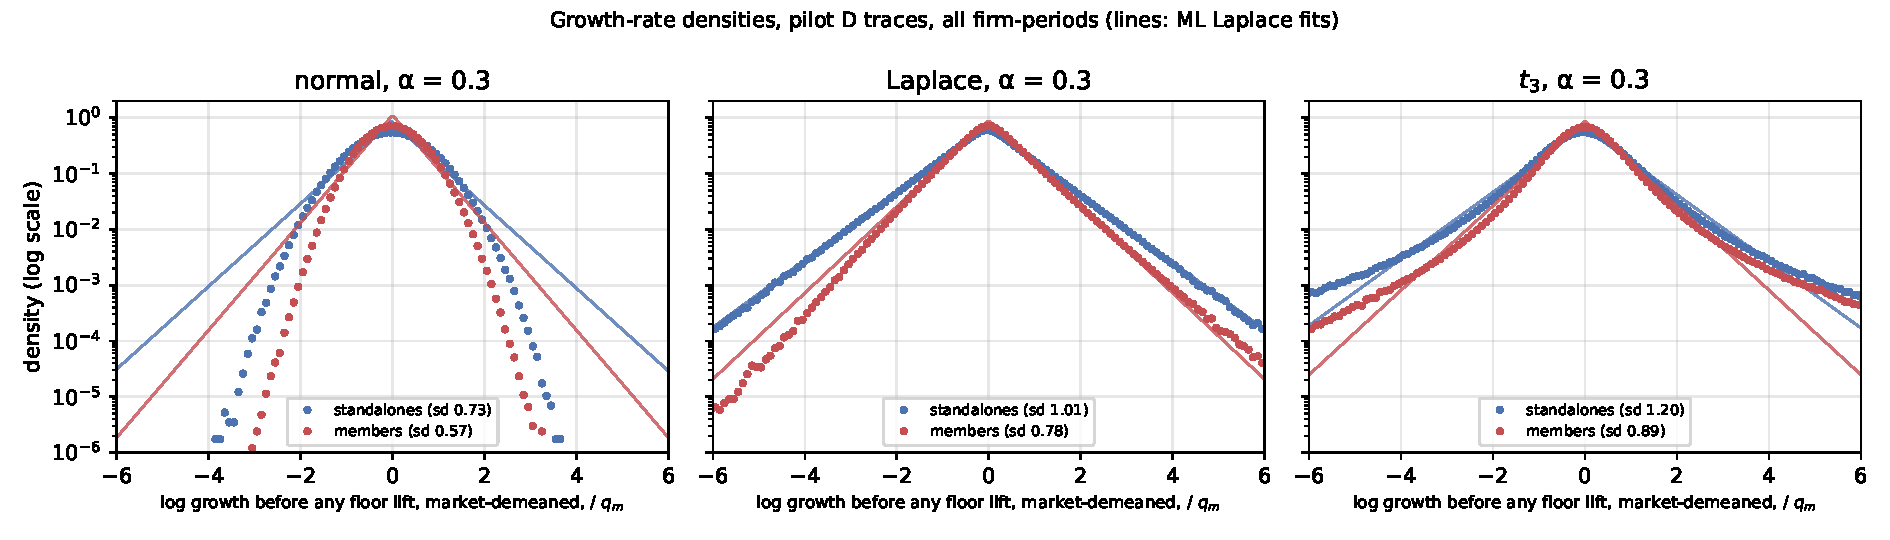
\includegraphics[width=\linewidth]{figures/appendix/growth_density_alpha0.3.pdf}
\caption{Densities of normalized per-period growth rates of members and standalones at $\alpha = 0.3$, log axis, with maximum-likelihood Laplace fits; one panel per family. 27 traced runs, moment rule.}
\label{fig:growth_density}
\end{figure}

\subsection{Concentration and rank mobility}\label{app:A17}

Table~\ref{tab:a18_concentration} gives the concentration measures behind Section~\ref{sec:results-distribution}. Within markets firms become more equal: the within-market Herfindahl index falls from 0.175--0.20 at $\alpha = 0$ to 0.14--0.17 at $\alpha = 0.3$ and 0.11--0.14 at $\alpha = 0.5$. Across the economy the units that own them become fewer and larger: the capital held by the largest ten per cent of owners, a conglomerate counted as one owner, goes from 0.65 to 0.65 (normal, with 0.67 at $\alpha = 0.3$), 0.66 to 0.74 (Laplace) and 0.68 to 0.79 ($t_3$) between $\alpha = 0$ and $0.5$; beyond $0.5$ it falls to 0.53 (normal) and 0.67 (Laplace) at $\alpha = 0.9$ while $t_3$ reaches 0.81, as the units' members grow more equal in size ($K_{\text{eff}}/K$ rises again to 0.68--0.71). Units sort by volatility and grow unequal: assortativity, the dispersion of members' market volatilities relative to that of a random set of the same size, falls from 0.60--0.61 at $\alpha = 0.01$ to 0.35--0.36 at $\alpha = 0.5$, because the consent test selects partners whose fluctuations are worth sharing from both sides; the effective number of members falls from 0.83--0.88 of $K$ to 0.64--0.68 over the same range as units accumulate a few large members and many recruits from the floor.

Tables~\ref{tab:a17_rank_mobility} and \ref{tab:a17b_rank_mobility_status} measure rank mobility from the 27 traced runs and nine traced $\alpha = 0$ runs: within each market, ranks of log share at an origin every 100 periods and 100 periods later, giving the Spearman correlation, the persistence of the top and bottom decile, leader turnover and the mean absolute rank change; a hit-free sample drops firms lifted at the floor in between and re-ranks the rest; the same by status at the origin; and the same for owning units across the economy. Pooling lowers rank mobility within markets in every family (lag-100 Spearman 0.16--0.33 at $\alpha = 0$ against 0.25--0.45 at $\alpha = 0.3$; top-decile persistence 0.31--0.48 against 0.36--0.53), partly through fewer floor lifts (0.68--0.83 of firms lifted within 100 periods against 0.52--0.71) and partly through slower movement among going concerns (members' ranks move 9--20\% less than standalones'); and it makes the top decile of owners markedly more persistent (0.32--0.49 against 0.67--0.69). Mobility is high in every cell and ranks are nearly independent at lag 500. The per-firm rank range and rank standard deviation of the earlier draft, recomputed on the traces, are at their ceiling in the floored economy and move the same way.

\begin{table}[htbp]
\centering
\caption{Concentration within markets and across owners}
\label{tab:a18_concentration}
\small
\begin{tabular}{lrrrrr}
\toprule
Family & $\alpha$ & \makecell[b]{HHI within\\{}markets} & \makecell[b]{Top-decile\\{}owners' share} & $K_{\text{eff}}/K$ & Assortativity \\
\midrule
normal & 0 & 0.175 & 0.65 & -- & -- \\
 & 0.1 & 0.164 & 0.67 & 0.75 & 0.49 \\
 & 0.3 & 0.139 & 0.67 & 0.68 & 0.39 \\
 & 0.5 & 0.109 & 0.65 & 0.65 & 0.36 \\
Laplace & 0 & 0.179 & 0.66 & -- & -- \\
 & 0.1 & 0.168 & 0.72 & 0.73 & 0.49 \\
 & 0.3 & 0.144 & 0.73 & 0.68 & 0.40 \\
 & 0.5 & 0.113 & 0.74 & 0.64 & 0.35 \\
$t_3$ & 0 & 0.201 & 0.68 & -- & -- \\
 & 0.1 & 0.191 & 0.74 & 0.74 & 0.52 \\
 & 0.3 & 0.167 & 0.77 & 0.70 & 0.42 \\
 & 0.5 & 0.136 & 0.79 & 0.67 & 0.35 \\
\bottomrule
\end{tabular}
\end{table}

\begin{sidewaystable}[htbp]
\centering
\caption{Rank mobility within markets and persistence of owners, lag 100 periods}
\label{tab:a17_rank_mobility}
\small
\begin{tabular}{lrrrrrrrr}
\toprule
Family & $\alpha$ & \makecell[b]{Spearman\\{}(all /\\{}hit-free)} & \makecell[b]{Top-decile\\{}persistence\\{}(all / hit-free)} & \makecell[b]{Leader\\{}turnover\\{}(all / hit-free)} & \makecell[b]{Mean\\{}rank\\{}change} & \makecell[b]{Share\\{}lifted\\{}within 100} & \makecell[b]{Owners:\\{}Spearman} & \makecell[b]{Owners:\\{}top-decile\\{}persistence} \\
\midrule
normal & 0 & 0.33 / 0.41 & 0.48 / 0.45 & 0.60 / 0.62 & 13.1 & 0.68 & 0.33 & 0.49 \\
 & 0.05 & 0.34 / 0.42 & 0.48 / 0.46 & 0.59 / 0.62 & 12.9 & 0.66 & 0.38 & 0.63 \\
 & 0.1 & 0.36 / 0.43 & 0.49 / 0.47 & 0.59 / 0.62 & 12.7 & 0.63 & 0.38 & 0.66 \\
 & 0.3 & 0.45 / 0.49 & 0.53 / 0.50 & 0.58 / 0.59 & 11.6 & 0.52 & 0.40 & 0.69 \\
Laplace & 0 & 0.21 / 0.31 & 0.35 / 0.36 & 0.73 / 0.71 & 14.4 & 0.78 & 0.20 & 0.37 \\
 & 0.05 & 0.22 / 0.31 & 0.36 / 0.35 & 0.73 / 0.71 & 14.3 & 0.77 & 0.24 & 0.55 \\
 & 0.1 & 0.24 / 0.32 & 0.37 / 0.35 & 0.72 / 0.72 & 14.1 & 0.75 & 0.24 & 0.59 \\
 & 0.3 & 0.32 / 0.35 & 0.41 / 0.37 & 0.71 / 0.71 & 13.2 & 0.64 & 0.27 & 0.68 \\
$t_3$ & 0 & 0.16 / 0.29 & 0.31 / 0.32 & 0.77 / 0.74 & 14.9 & 0.83 & 0.16 & 0.32 \\
 & 0.05 & 0.17 / 0.29 & 0.32 / 0.32 & 0.77 / 0.74 & 14.8 & 0.81 & 0.19 & 0.50 \\
 & 0.1 & 0.19 / 0.29 & 0.32 / 0.32 & 0.77 / 0.73 & 14.7 & 0.80 & 0.19 & 0.55 \\
 & 0.3 & 0.25 / 0.32 & 0.36 / 0.36 & 0.75 / 0.72 & 13.9 & 0.71 & 0.23 & 0.67 \\
\bottomrule
\end{tabular}
\par\smallskip\begin{minipage}{0.95\linewidth}\footnotesize Pooling lowers rank mobility within markets in every family (persistence rises with the sharing rate) and makes the top decile of owners more persistent; the hit-free columns show that part, not all, of the fall is fewer recapitalizations at the floor.\end{minipage}
\end{sidewaystable}

\begin{sidewaystable}[htbp]
\centering
\caption{Rank mobility by status at the origin, lag 100 periods}
\label{tab:a17b_rank_mobility_status}
\small
\begin{tabular}{lrrrrr}
\toprule
Family & $\alpha$ & \makecell[b]{Top-decile persistence\\{}(member / standalone)} & \makecell[b]{Mean rank change\\{}(member / standalone)} & \makecell[b]{Share lifted within 100\\{}(member / standalone)} & \makecell[b]{Members' share\\{}of the top decile} \\
\midrule
normal & 0.05 & 0.46 / 0.65 & 12.2 / 14.0 & 0.55 / 0.83 & 0.87 \\
 & 0.1 & 0.48 / 0.63 & 12.0 / 14.1 & 0.52 / 0.84 & 0.94 \\
 & 0.3 & 0.53 / 0.48 & 10.9 / 13.6 & 0.41 / 0.82 & 0.99 \\
Laplace & 0.05 & 0.35 / 0.43 & 13.6 / 15.1 & 0.67 / 0.88 & 0.88 \\
 & 0.1 & 0.37 / 0.36 & 13.4 / 15.1 & 0.65 / 0.89 & 0.93 \\
 & 0.3 & 0.41 / 0.30 & 12.5 / 14.9 & 0.54 / 0.87 & 0.97 \\
$t_3$ & 0.05 & 0.31 / 0.34 & 14.2 / 15.5 & 0.73 / 0.90 & 0.84 \\
 & 0.1 & 0.33 / 0.29 & 14.0 / 15.6 & 0.70 / 0.91 & 0.89 \\
 & 0.3 & 0.37 / 0.28 & 13.1 / 15.3 & 0.60 / 0.89 & 0.95 \\
\bottomrule
\end{tabular}
\par\smallskip\begin{minipage}{0.95\linewidth}\footnotesize Members' ranks move less than standalones' in every cell; the standalone top-decile figures rest on few firms, since members hold 84--99\% of the top decile.\end{minipage}
\end{sidewaystable}


\subsection{Scope without consent: the accept rule}\label{app:accept}

Under the accept rule every feasible proposal merges and no one leaves by choice; everything else is unchanged. It is a control without knowledge, not a behavioural alternative: it shows the scope the floor and the one-firm-per-market constraint alone permit. Table~\ref{tab:a19_accept} sets it beside the moment and loggain rules on the main power-law cells (45 runs on the main cells' seeds): $K_{\text{accept}}$ is 12.4--28.2 against 3.5--7.7, above the equal-members reference in every normal and Laplace cell and below it under $t_3$ (0.3--0.6 of $K^*$). The extra mergers are solo entries of floor-sized firms into existing units (86--89\% of the control's entries are at the floor); unit--unit mergers do not rise with consent off, because consolidated units occupy most markets and clash. The pooled share rises by 0.02--0.11, the Hill exponent by 0.00--0.04, the within-market Herfindahl index falls by 0.004--0.012, and the members' floor-hit rate rises slightly. Table~\ref{tab:decomposition-accept} is the four-part re-cut of Table~\ref{tab:decomposition} that separates what the environment permits from what consent withholds.

\begin{sidewaystable}[htbp]
\centering
\caption{The accept rule against the moment and loggain rules}
\label{tab:a19_accept}
\small
\begin{tabular}{lrrrrrrrrrr}
\toprule
Family & $\alpha$ & \makecell[b]{K:\\{}accept} & moment & loggain & \makecell[b]{Pooled:\\{}accept} & moment & \makecell[b]{Hill:\\{}accept} & moment & \makecell[b]{HHI within:\\{}accept} & moment \\
\midrule
normal & 0.1 & 17.6 & 3.7 & 3.0 & 0.95 & 0.85 & 1.12 & 1.11 & 0.160 & 0.164 \\
 & 0.3 & 22.2 & 5.5 & 4.3 & 0.97 & 0.94 & 1.21 & 1.21 & 0.133 & 0.139 \\
 & 0.5 & 28.2 & 7.7 & 6.3 & 0.98 & 0.96 & 1.37 & 1.34 & 0.106 & 0.109 \\
Laplace & 0.1 & 13.8 & 3.7 & 3.0 & 0.93 & 0.85 & 1.11 & 1.11 & 0.164 & 0.168 \\
 & 0.3 & 18.1 & 5.4 & 4.0 & 0.95 & 0.91 & 1.23 & 1.19 & 0.135 & 0.144 \\
 & 0.5 & 24.3 & 7.8 & 5.9 & 0.97 & 0.93 & 1.35 & 1.34 & 0.109 & 0.113 \\
$t_3$ & 0.1 & 12.4 & 3.5 & 2.9 & 0.91 & 0.83 & 1.04 & 1.03 & 0.188 & 0.191 \\
 & 0.3 & 16.2 & 4.8 & 3.7 & 0.94 & 0.90 & 1.13 & 1.12 & 0.160 & 0.167 \\
 & 0.5 & 21.8 & 6.8 & 5.1 & 0.96 & 0.92 & 1.26 & 1.22 & 0.127 & 0.136 \\
\bottomrule
\end{tabular}
\end{sidewaystable}

\begin{sidewaystable}[htbp]
\centering
\caption{Four-part decomposition of the distance to the equal-members reference, power-law cost; medians over five replications}
\label{tab:decomposition-accept}
\small
\begin{tabular}{lrrrrrrrrrr}
\toprule
Family & $\alpha$ & $K^*$ & $K_{\text{accept}}$ & $K_{\text{hom}}$ & $K$ & $K_{\text{loggain}}$ & Environment & Consent & Transfer & Verifiability \\
\midrule
normal & 0.1 & 8 & 17.6 & 3.8 & 3.7 & 3.0 & -9.6 (-194\%) & 13.8 (279\%) & 0.1 (2\%) & 0.6 (13\%) \\
 & 0.3 & 12 & 22.2 & 5.6 & 5.5 & 4.3 & -10.2 (-133\%) & 16.7 (216\%) & 0.1 (1\%) & 1.2 (15\%) \\
 & 0.5 & 13 & 28.2 & 8.0 & 7.7 & 6.3 & -15.2 (-228\%) & 20.2 (304\%) & 0.3 (4\%) & 1.4 (20\%) \\
\midrule
Laplace & 0.1 & 10 & 13.8 & 3.8 & 3.7 & 3.0 & -3.8 (-55\%) & 10.0 (143\%) & 0.1 (1\%) & 0.7 (10\%) \\
 & 0.3 & 16 & 18.1 & 5.5 & 5.4 & 4.0 & -2.1 (-18\%) & 12.6 (105\%) & 0.1 (1\%) & 1.4 (12\%) \\
 & 0.5 & 20 & 24.3 & 8.2 & 7.8 & 5.9 & -4.3 (-31\%) & 16.1 (115\%) & 0.4 (3\%) & 1.8 (13\%) \\
\midrule
$t_3$ & 0.1 & 20 & 12.4 & 3.5 & 3.5 & 2.9 & 7.6 (44\%) & 8.9 (52\%) & 0.0 (0\%) & 0.6 (4\%) \\
 & 0.3 & 47 & 16.2 & 4.9 & 4.8 & 3.7 & 30.8 (71\%) & 11.3 (26\%) & 0.1 (0\%) & 1.2 (3\%) \\
 & 0.5 & 50 & 21.8 & 7.0 & 6.8 & 5.1 & 28.2 (63\%) & 14.8 (33\%) & 0.2 (0\%) & 1.7 (4\%) \\
\bottomrule
\end{tabular}
\par\smallskip\begin{minipage}{0.95\linewidth}\footnotesize Environment $= K^* - K_{\text{accept}}$, consent $= K_{\text{accept}} - K_{\text{hom}}$, transfer $= K_{\text{hom}} - K$, verifiability $= K - K_{\text{loggain}}$; shares in parentheses are of $K^* - K_{\text{loggain}}$ (the four parts sum to it). $K_{\text{accept}}$: heterogeneous economy, every feasible proposal accepted and no voluntary exit (a control without knowledge). A negative environment part means the environment alone permits units larger than $K^*$. The consent part compares the heterogeneous accept economy with the homogeneous moment economy, so it also holds the homogeneous-heterogeneous difference of the accept rule.\end{minipage}
\end{sidewaystable}


\subsection{The sharing rate}\label{app:alpha}

Table~\ref{tab:endogenous} gives the endogenous-$\alpha$ block under the power-law cost and Table~\ref{tab:a13_endogenous} under all four cost forms and both rules. Units that choose their rate reach 14--18 mean members under the power-law cost, with 95--98\% of capital pooled and a tail exponent of 1.8--2.1. This is the scope that a rate near 0.9 implies, not a separate effect: along the fixed-rate grid $K$ rises from 5.4 at $\alpha = 0.3$ to 7.8 at $0.5$, and the fixed $\alpha = 0.9$ cell reproduces the endogenous block (Table~\ref{tab:robustness-b}). The ordering across families is the same as elsewhere: the heaviest tails choose a slightly lower rate and reach a smaller scope. The exponential-cost cells reach $K = 16$--23 at a lower pooled share (81--92\%). Neither heterogeneity among members nor the volatility of their markets drives the choice: across 7,630 units active at the end of a run, the Spearman correlation of a unit's time-averaged rate with the dispersion of its members' volatilities is $-0.14$ to $0.00$, and with their mean volatility 0.04--0.10. Under the loggain rule the latter was 0.14--0.26: units in more volatile markets pooled more, not because the optimum differed, it is full pooling at every volatility level, but because only there was the gain from a higher rate large enough to show through the window's noise.

\begin{table}[htbp]
\centering
\caption{The sharing rate units choose}
\label{tab:endogenous}
\small
\begin{tabular}{lrrrrrrr}
\toprule
Family & $\bar\alpha$ & median & share at 1 & $K$ & Pooled & Hill & $\rho(\alpha, \bar q)$ \\
\midrule
normal & 0.93 & 0.90 & 0.22 & 16.9 & 0.98 & 2.05 & 0.10 \\
Laplace & 0.92 & 0.90 & 0.14 & 18.0 & 0.97 & 2.07 & 0.05 \\
$t_3$ & 0.91 & 0.90 & 0.12 & 14.3 & 0.95 & 1.83 & 0.04 \\
\bottomrule
\end{tabular}
\par\smallskip\begin{minipage}{0.95\linewidth}\footnotesize Endogenous-$\alpha$ block, power-law cost, start $\alpha_C = 0.1$; adopted $\alpha$ over unit-periods; share at 1: unit-periods at $\alpha_C = 1$. $\rho$: Spearman correlation of a unit's time-averaged rate with the mean IQR of its members' markets, over the 2,468 / 2,319 / 2,843 units alive at $T$ (normal / Laplace / $t_3$). For comparison, the fixed $\alpha = 0.9$ cell gives $K = 16.0$, Hill 1.98; $K = 17.2$, Hill 1.94; $K = 13.9$, Hill 1.78 (same order).\end{minipage}
\end{table}

\begin{sidewaystable}[htbp]
\centering
\caption{Endogenous $\alpha$ by cost form}
\label{tab:a13_endogenous}
\small
\begin{tabular}{lrrrrrrr}
\toprule
Family & Cost form & $\bar\alpha$ & \makecell[b]{median,\\{}moment / loggain} & \makecell[b]{share\\{}at 1} & \makecell[b]{K,\\{}moment / loggain} & Pooled & Hill \\
\midrule
normal & power law & 0.93 & 0.90 / 0.85 & 0.22 & 16.9 / 12.1 & 0.98 & 2.05 \\
 & linear & 0.93 & 0.90 / 0.85 & 0.23 & 17.2 / 11.8 & 0.98 & 2.07 \\
 & quadratic & 0.93 & 0.90 / 0.85 & 0.20 & 17.5 / 12.6 & 0.98 & 2.02 \\
 & exponential & 0.94 & 0.95 / 0.80 & 0.24 & 23.2 / 20.5 & 0.81 & 1.88 \\
Laplace & power law & 0.92 & 0.90 / 0.80 & 0.14 & 18.0 / 11.5 & 0.97 & 2.07 \\
 & linear & 0.92 & 0.90 / 0.85 & 0.13 & 18.5 / 11.8 & 0.97 & 2.06 \\
 & quadratic & 0.93 & 0.90 / 0.80 & 0.17 & 18.8 / 12.4 & 0.97 & 2.06 \\
 & exponential & 0.93 & 0.95 / 0.85 & 0.16 & 22.1 / 16.0 & 0.91 & 2.00 \\
$t_3$ & power law & 0.91 & 0.90 / 0.80 & 0.12 & 14.3 / 8.8 & 0.95 & 1.83 \\
 & linear & 0.92 & 0.90 / 0.80 & 0.14 & 14.3 / 8.7 & 0.95 & 1.84 \\
 & quadratic & 0.91 & 0.90 / 0.80 & 0.11 & 14.4 / 9.2 & 0.95 & 1.84 \\
 & exponential & 0.91 & 0.90 / 0.80 & 0.10 & 16.0 / 10.4 & 0.92 & 1.83 \\
\bottomrule
\end{tabular}
\end{sidewaystable}


\section{Robustness}\label{app:robustness}

\subsection{Summary}

Tables~\ref{tab:robustness} and \ref{tab:robustness-b} summarize every block at $\alpha = 0.3$ (the endogenous-$\alpha$ block at its adopted rate) against the Laplace power-law baseline. The rest of this section gives each block in full.

\begin{table}[htbp]
\centering
\caption{Robustness: environment and decision parameters}
\label{tab:robustness}
\small
\begin{tabular}{llrrrr}
\toprule
Block & Variant & $K$ & Pooled & Hill & Floor exits \\
\midrule
cost form & linear & 5.2 & 0.91 & 1.18 & 35 \\
 & quadratic & 5.9 & 0.92 & 1.19 & 36 \\
 & exponential & 6.1 & 0.88 & 1.21 & 36 \\
\midrule
cost level & $\times 0.5$ & 6.0 & 0.92 & 1.20 & 35 \\
 & $\times 2$ & 4.7 & 0.91 & 1.19 & 35 \\
 & $\times 5$ & 3.9 & 0.87 & 1.17 & 33 \\
 & $\times 10$ & 3.3 & 0.79 & 1.15 & 33 \\
 & $\times 20$ & 2.8 & 0.67 & 1.13 & 33 \\
\midrule
window $l$ & 20 & 4.8 & 0.91 & 1.19 & 35 \\
 & 100 & 5.8 & 0.92 & 1.20 & 37 \\
 & 200 & 6.1 & 0.93 & 1.21 & 34 \\
 & 500 & 6.6 & 0.92 & 1.20 & 38 \\
\midrule
search $p$ & 0.2 & 6.8 & 0.97 & 1.18 & 62 \\
 & 1 & 8.0 & 0.98 & 1.18 & 116 \\
\midrule
correlation & cross-market 0.3 & 5.3 & 0.91 & 1.21 & 36 \\
\midrule
floor $c$ & 0.10 & 5.6 & 0.93 & 1.13 & 32 \\
 & 0.35 & 4.4 & 0.74 & 1.66 & 60 \\
\midrule
economy size $(M, N)$ & (25, 25) & 5.6 & 0.96 & 1.22 & 7 \\
 & (100, 25) & 6.2 & 0.96 & 1.24 & 23 \\
 & (25, 100) & 4.7 & 0.88 & 1.16 & 44 \\
 & (100, 100) & 5.2 & 0.89 & 1.17 & 170 \\
\bottomrule
\end{tabular}
\par\smallskip\begin{minipage}{0.95\linewidth}\footnotesize At $\alpha = 0.3$, Laplace shocks, power-law cost unless stated, moment rule; medians over five replications. Baseline: $K = 5.4$, pooled 0.91, Hill 1.19, 36 floor exits per period. \end{minipage}
\end{table}

\begin{table}[htbp]
\centering
\caption{Robustness: contract, shock family and decision rule}
\label{tab:robustness-b}
\small
\begin{tabular}{llrrrr}
\toprule
Block & Variant & $K$ & Pooled & Hill & Floor exits \\
\midrule
equal split (normal) & linear & 2.9 & 0.29 & 1.12 & 21 \\
 & quadratic & 3.0 & 0.33 & 1.14 & 24 \\
 & exponential & 2.8 & 0.24 & 1.09 & 21 \\
 & power law & 3.0 & 0.33 & 1.13 & 24 \\
\midrule
endogenous $\alpha$ & normal & 16.9 & 0.98 & 2.05 & 2 \\
 & Laplace & 18.0 & 0.97 & 2.07 & 4 \\
 & $t_3$ & 14.3 & 0.95 & 1.83 & 11 \\
\midrule
fixed $\alpha = 0.9$ & normal & 16.0 & 0.98 & 1.98 & 2 \\
 & Laplace & 17.2 & 0.97 & 1.94 & 5 \\
 & $t_3$ & 13.9 & 0.95 & 1.78 & 11 \\
\midrule
tail weight $\nu$ (Student-$t$) & 2.5 & 4.1 & 0.85 & 1.02 & 54 \\
 & 3 & 4.8 & 0.90 & 1.12 & 42 \\
 & 4 & 5.3 & 0.92 & 1.17 & 33 \\
\midrule
homogeneous markets & normal & 5.6 & 0.94 & 1.20 & 22 \\
 & Laplace & 5.5 & 0.91 & 1.19 & 34 \\
 & $t_3$ & 4.9 & 0.89 & 1.10 & 42 \\
\midrule
loggain rule & normal & 4.3 & 0.73 & 1.17 & 26 \\
 & Laplace & 4.0 & 0.78 & 1.16 & 37 \\
 & $t_3$ & 3.7 & 0.77 & 1.10 & 43 \\
\bottomrule
\end{tabular}
\par\smallskip\begin{minipage}{0.95\linewidth}\footnotesize Conventions as in Table~\ref{tab:robustness}; family rows are at $\alpha = 0.3$ except the endogenous-$\alpha$ block. Homogeneous markets: every market at $q = 0.20$.\end{minipage}
\end{table}


\subsection{Cost form and level}\label{app:cost}

Table~\ref{tab:a10_cost_forms} gives the four cost forms at equal $\Phi(40)$ for all three families; the form moves scope by under one member. Table~\ref{tab:costlevel} runs the power-law level from $\times 0.5$ to $\times 20$ at $\alpha = 0.3$ under both rules with the equal-members reference recomputed at each level: scope falls by about 0.6 members per doubling of the cost and the ratio $K/K^*$ rises, but the reference is never reached, because the reference falls with the cost as well. Table~\ref{tab:a10b_cost_levels} gives the $\times 0.5$ and $\times 2$ cells for every form, with $b_0$ alone scaled (power law and exponential: the whole schedule) or all coefficients scaled (linear, quadratic).

\begin{table}[htbp]
\centering
\caption{Cost forms at equal $\Phi$(40), $\alpha$ = 0.3}
\label{tab:a10_cost_forms}
\small
\begin{tabular}{lrrrrr}
\toprule
Family & Cost form & K & Pooled & Hill & Acceptance \\
\midrule
normal & power law & 5.5 & 0.94 & 1.21 & 0.29 \\
normal & linear & 5.3 & 0.93 & 1.21 & 0.26 \\
normal & quadratic & 6.4 & 0.94 & 1.22 & 0.34 \\
normal & exponential & 6.6 & 0.87 & 1.22 & 0.35 \\
Laplace & power law & 5.4 & 0.91 & 1.19 & 0.40 \\
Laplace & linear & 5.2 & 0.91 & 1.18 & 0.39 \\
Laplace & quadratic & 5.9 & 0.92 & 1.19 & 0.42 \\
Laplace & exponential & 6.1 & 0.88 & 1.21 & 0.44 \\
$t_3$ & power law & 4.8 & 0.90 & 1.12 & 0.44 \\
$t_3$ & linear & 4.6 & 0.88 & 1.10 & 0.46 \\
$t_3$ & quadratic & 4.9 & 0.88 & 1.09 & 0.49 \\
$t_3$ & exponential & 5.2 & 0.86 & 1.11 & 0.47 \\
\bottomrule
\end{tabular}
\end{table}

\begin{table}[htbp]
\centering
\caption{Cost level, power-law form, $\alpha = 0.3$; medians over five replications}
\label{tab:costlevel}
\small
\begin{tabular}{lrrrrrrrr}
\toprule
Family & Cost level & $K$ & $K$, loggain & $K^*$ & $K/K^*$ & Pooled & Accept. & Hill \\
\midrule
Laplace & 0.5 & 6.0 & 4.3 & -- & -- & 0.92 & 0.42 & 1.20 \\
 & 1 & 5.4 & 4.0 & 16 & 0.34 & 0.91 & 0.40 & 1.19 \\
 & 2 & 4.7 & 3.7 & -- & -- & 0.91 & 0.36 & 1.19 \\
 & 5 & 3.9 & 3.1 & 8 & 0.49 & 0.87 & 0.31 & 1.17 \\
 & 10 & 3.3 & 2.8 & 6 & 0.55 & 0.79 & 0.29 & 1.15 \\
 & 20 & 2.8 & 2.5 & 4 & 0.70 & 0.67 & 0.29 & 1.13 \\
\midrule
$t_3$ & 1 & 4.8 & 3.7 & 47 & 0.10 & 0.90 & 0.44 & 1.12 \\
 & 5 & 3.7 & 3.0 & 10 & 0.37 & 0.85 & 0.38 & 1.10 \\
 & 10 & 3.3 & 2.8 & 7 & 0.47 & 0.80 & 0.37 & 1.07 \\
 & 20 & 2.8 & 2.5 & 5 & 0.57 & 0.70 & 0.36 & 1.05 \\
\bottomrule
\end{tabular}
\end{table}

\begin{table}[htbp]
\centering
\caption{Cost level $\times$0.5 and $\times$2, Laplace}
\label{tab:a10b_cost_levels}
\small
\begin{tabular}{lrrrrrr}
\toprule
Scaled & Cost form & Level & $\alpha$ & K & Pooled & Acceptance \\
\midrule
$b_0$ only & exponential & $\times$0.5 & 0.1 & 4.5 & 0.75 & 0.46 \\
$b_0$ only & exponential & $\times$0.5 & 0.3 & 6.4 & 0.91 & 0.46 \\
$b_0$ only & exponential & $\times$0.5 & 0.5 & 9.5 & 0.94 & 0.44 \\
$b_0$ only & exponential & $\times$2 & 0.1 & 3.6 & 0.38 & 0.32 \\
$b_0$ only & exponential & $\times$2 & 0.3 & 5.5 & 0.81 & 0.42 \\
$b_0$ only & exponential & $\times$2 & 0.5 & 8.0 & 0.91 & 0.40 \\
$b_0$ only & linear & $\times$0.5 & 0.1 & 3.6 & 0.82 & 0.42 \\
$b_0$ only & linear & $\times$0.5 & 0.3 & 5.3 & 0.91 & 0.39 \\
$b_0$ only & linear & $\times$0.5 & 0.5 & 7.7 & 0.94 & 0.37 \\
$b_0$ only & linear & $\times$2 & 0.1 & 3.6 & 0.82 & 0.44 \\
$b_0$ only & linear & $\times$2 & 0.3 & 5.2 & 0.91 & 0.41 \\
$b_0$ only & linear & $\times$2 & 0.5 & 7.6 & 0.93 & 0.39 \\
$b_0$ only & power law & $\times$0.5 & 0.1 & 4.1 & 0.88 & 0.43 \\
$b_0$ only & power law & $\times$0.5 & 0.3 & 6.0 & 0.92 & 0.42 \\
$b_0$ only & power law & $\times$0.5 & 0.5 & 8.7 & 0.94 & 0.40 \\
$b_0$ only & power law & $\times$2 & 0.1 & 3.3 & 0.80 & 0.39 \\
$b_0$ only & power law & $\times$2 & 0.3 & 4.7 & 0.91 & 0.36 \\
$b_0$ only & power law & $\times$2 & 0.5 & 6.7 & 0.94 & 0.32 \\
$b_0$ only & quadratic & $\times$0.5 & 0.1 & 4.2 & 0.87 & 0.47 \\
$b_0$ only & quadratic & $\times$0.5 & 0.3 & 5.9 & 0.91 & 0.45 \\
$b_0$ only & quadratic & $\times$0.5 & 0.5 & 8.4 & 0.93 & 0.41 \\
$b_0$ only & quadratic & $\times$2 & 0.1 & 4.2 & 0.83 & 0.46 \\
$b_0$ only & quadratic & $\times$2 & 0.3 & 5.9 & 0.91 & 0.44 \\
$b_0$ only & quadratic & $\times$2 & 0.5 & 8.3 & 0.94 & 0.41 \\
all coefficients & linear & $\times$0.5 & 0.1 & 4.0 & 0.87 & 0.44 \\
all coefficients & linear & $\times$0.5 & 0.3 & 6.0 & 0.92 & 0.42 \\
all coefficients & linear & $\times$0.5 & 0.5 & 8.9 & 0.94 & 0.40 \\
all coefficients & linear & $\times$2 & 0.1 & 3.2 & 0.75 & 0.40 \\
all coefficients & linear & $\times$2 & 0.3 & 4.6 & 0.90 & 0.35 \\
all coefficients & linear & $\times$2 & 0.5 & 6.6 & 0.93 & 0.32 \\
all coefficients & quadratic & $\times$0.5 & 0.1 & 4.5 & 0.88 & 0.48 \\
all coefficients & quadratic & $\times$0.5 & 0.3 & 6.3 & 0.92 & 0.46 \\
all coefficients & quadratic & $\times$0.5 & 0.5 & 9.1 & 0.94 & 0.43 \\
all coefficients & quadratic & $\times$2 & 0.1 & 3.9 & 0.81 & 0.44 \\
all coefficients & quadratic & $\times$2 & 0.3 & 5.4 & 0.91 & 0.41 \\
all coefficients & quadratic & $\times$2 & 0.5 & 7.6 & 0.93 & 0.37 \\
\bottomrule
\end{tabular}
\end{table}


\subsection{Floor level, correlation and economy size}\label{app:environment}

Tables~\ref{tab:a11a_floor}--\ref{tab:a11c_size}, Laplace shocks and power-law cost. The floor level sets the tail exponent and little else: scope moves by $+3\%$ at $c = 0.10$ and $-19\%$ at $c = 0.35$ while the Hill exponent moves from 1.13 to 1.66 at $\alpha = 0.3$. Cross-market correlation of 0.3 leaves every outcome within 0.2 of the baseline. Economy size matters through the number of firms per market and barely through the number of markets, with the floor recalibrated to $c^*(N)$.

\begin{table}[htbp]
\centering
\caption{Floor level}
\label{tab:a11a_floor}
\small
\begin{tabular}{lrrrrrr}
\toprule
c & $\alpha$ & K & Pooled & Hill & Acceptance & \makecell[b]{Floor exits\\{}/ period} \\
\midrule
0.1 & 0.1 & 3.8 & 0.87 & 1.05 & 0.38 & 42.3 \\
0.1 & 0.3 & 5.6 & 0.93 & 1.13 & 0.36 & 31.5 \\
0.1 & 0.5 & 8.2 & 0.95 & 1.29 & 0.34 & 20.3 \\
0.35 & 0.1 & 3.3 & 0.68 & 1.55 & 0.60 & 69.9 \\
0.35 & 0.3 & 4.4 & 0.74 & 1.66 & 0.56 & 59.9 \\
0.35 & 0.5 & 5.8 & 0.78 & 1.80 & 0.53 & 47.7 \\
\bottomrule
\end{tabular}
\end{table}

\begin{table}[htbp]
\centering
\caption{Cross-market correlation 0.3}
\label{tab:a11b_correlation}
\small
\begin{tabular}{lrrrrrr}
\toprule
correlation & $\alpha$ & K & Pooled & Hill & Acceptance & \makecell[b]{Floor exits\\{}/ period} \\
\midrule
0.3 & 0.1 & 3.7 & 0.85 & 1.10 & 0.42 & 47.1 \\
0.3 & 0.3 & 5.3 & 0.91 & 1.21 & 0.40 & 36.3 \\
0.3 & 0.5 & 7.6 & 0.94 & 1.34 & 0.37 & 24.3 \\
\bottomrule
\end{tabular}
\end{table}

\begin{table}[htbp]
\centering
\caption{Economy size with $c^*$(N)}
\label{tab:a11c_size}
\small
\begin{tabular}{lrrrrrr}
\toprule
M / N & $\alpha$ & K & Pooled & Hill & Acceptance & \makecell[b]{Floor exits\\{}/ period} \\
\midrule
25 / 25 & 0.1 & 3.8 & 0.91 & 1.13 & 0.38 & 9.0 \\
25 / 25 & 0.3 & 5.6 & 0.96 & 1.22 & 0.40 & 6.5 \\
25 / 25 & 0.5 & 8.0 & 0.97 & 1.45 & 0.39 & 3.9 \\
25 / 100 & 0.1 & 3.5 & 0.81 & 1.10 & 0.52 & 53.9 \\
25 / 100 & 0.3 & 4.7 & 0.88 & 1.16 & 0.52 & 43.7 \\
25 / 100 & 0.5 & 6.3 & 0.91 & 1.26 & 0.50 & 31.1 \\
100 / 25 & 0.1 & 4.0 & 0.91 & 1.12 & 0.29 & 33.3 \\
100 / 25 & 0.3 & 6.2 & 0.96 & 1.24 & 0.24 & 23.1 \\
100 / 25 & 0.5 & 9.4 & 0.97 & 1.45 & 0.20 & 13.0 \\
100 / 100 & 0.1 & 3.6 & 0.82 & 1.09 & 0.46 & 215.9 \\
100 / 100 & 0.3 & 5.2 & 0.89 & 1.17 & 0.40 & 170.2 \\
100 / 100 & 0.5 & 7.6 & 0.91 & 1.28 & 0.35 & 118.3 \\
\bottomrule
\end{tabular}
\end{table}


\subsection{Homogeneous markets}\label{app:homogeneous}

Table~\ref{tab:a8_homogeneous}: every market at $q = 0.20$, power-law cost, both rules. The homogeneous economy is the $K_{\text{hom}}$ of Table~\ref{tab:decomposition}; it exceeds the heterogeneous base case by 0.0--0.4 members, which bounds the transfer conflict between members of unequal volatility.

\begin{table}[htbp]
\centering
\caption{Homogeneous block}
\label{tab:a8_homogeneous}
\small
\begin{tabular}{lrrrrrr}
\toprule
Family & Rule & $\alpha$ & K & Pooled & Acceptance & Hill \\
\midrule
normal & moment & 0.05 & 3.2 & 0.77 & 0.30 & 1.09 \\
normal & moment & 0.1 & 3.8 & 0.86 & 0.29 & 1.10 \\
normal & moment & 0.3 & 5.6 & 0.94 & 0.26 & 1.20 \\
normal & moment & 0.5 & 8.0 & 0.96 & 0.23 & 1.34 \\
normal & loggain & 0.05 & 2.8 & 0.49 & 0.32 & 1.07 \\
normal & loggain & 0.1 & 3.2 & 0.58 & 0.32 & 1.08 \\
normal & loggain & 0.3 & 4.6 & 0.75 & 0.26 & 1.18 \\
normal & loggain & 0.5 & 6.8 & 0.93 & 0.22 & 1.33 \\
Laplace & moment & 0.05 & 3.3 & 0.80 & 0.42 & 1.07 \\
Laplace & moment & 0.1 & 3.8 & 0.86 & 0.41 & 1.10 \\
Laplace & moment & 0.3 & 5.5 & 0.91 & 0.38 & 1.19 \\
Laplace & moment & 0.5 & 8.2 & 0.93 & 0.35 & 1.33 \\
Laplace & loggain & 0.05 & 2.8 & 0.57 & 0.42 & 1.07 \\
Laplace & loggain & 0.1 & 3.1 & 0.64 & 0.41 & 1.09 \\
Laplace & loggain & 0.3 & 4.2 & 0.80 & 0.35 & 1.17 \\
Laplace & loggain & 0.5 & 6.3 & 0.91 & 0.31 & 1.32 \\
$t_3$ & moment & 0.05 & 3.1 & 0.77 & 0.47 & 1.01 \\
$t_3$ & moment & 0.1 & 3.5 & 0.83 & 0.46 & 1.02 \\
$t_3$ & moment & 0.3 & 4.9 & 0.89 & 0.43 & 1.10 \\
$t_3$ & moment & 0.5 & 7.0 & 0.92 & 0.39 & 1.22 \\
$t_3$ & loggain & 0.05 & 2.7 & 0.57 & 0.46 & 1.00 \\
$t_3$ & loggain & 0.1 & 2.9 & 0.64 & 0.45 & 1.01 \\
$t_3$ & loggain & 0.3 & 3.8 & 0.79 & 0.40 & 1.08 \\
$t_3$ & loggain & 0.5 & 5.3 & 0.89 & 0.35 & 1.20 \\
\bottomrule
\end{tabular}
\end{table}


\subsection{Tail weight}\label{app:nu}

Table~\ref{tab:a9_nu}: Student-$t$ shocks with $\nu \in \{2.5, 3, 4\}$ at equal IQR, power-law cost, moment rule. The last two columns give the distribution of the window variance estimate relative to its population value over 200,000 i.i.d.\ 50-period windows at $q = 0.2$, and the share of windows in which it is below one half. Scope falls with tail weight while acceptance rises: under heavier tails firms are more willing to pool and less able to stay pooled, because members are recapitalized more often. Attrition, not consent, takes the scope.

\begin{sidewaystable}[htbp]
\centering
\caption{$\nu$ block}
\label{tab:a9_nu}
\small
\begin{tabular}{lrrrrrrrrr}
\toprule
$\nu$ & $\alpha$ & K & Pooled & Hill & Acceptance & \makecell[b]{Floor exits\\{}/ period} & \makecell[b]{Hazard\\{}ratio} & \makecell[b]{$\hat\sigma^2/\sigma^2$\\{}median [5\%, 95\%]} & \makecell[b]{share\\{}< $\tfrac12$} \\
\midrule
2.5 & 0.1 & 3.2 & 0.78 & 0.96 & 0.54 & 63.3 & 0.25 & 0.59 [0.29, 2.01] & 0.37 \\
 & 0.3 & 4.1 & 0.85 & 1.02 & 0.50 & 53.5 & 0.17 &  &  \\
 & 0.5 & 5.5 & 0.88 & 1.12 & 0.46 & 42.0 & 0.12 &  &  \\
3 & 0.1 & 3.5 & 0.83 & 1.03 & 0.47 & 53.1 & 0.19 & 0.77 [0.42, 1.98] & 0.13 \\
 & 0.3 & 4.8 & 0.90 & 1.12 & 0.44 & 42.5 & 0.13 &  &  \\
 & 0.5 & 6.8 & 0.92 & 1.22 & 0.41 & 31.2 & 0.08 &  &  \\
4 & 0.1 & 3.7 & 0.85 & 1.07 & 0.39 & 43.7 & 0.15 & 0.89 [0.53, 1.74] & 0.03 \\
 & 0.3 & 5.3 & 0.92 & 1.17 & 0.37 & 33.4 & 0.10 &  &  \\
 & 0.5 & 7.7 & 0.94 & 1.31 & 0.34 & 21.8 & 0.06 &  &  \\
\bottomrule
\end{tabular}
\end{sidewaystable}


\subsection{Equal sharing}\label{app:equalsplit}

Table~\ref{tab:a12_equal_split}: equal dollar splits of the net pool, normal shocks, four cost forms, with acceptance by proposal type (standalone--standalone, standalone--unit), voluntary exits, pool ruin (a unit's members capped at limited liability in a period) and the shortfall charged to the other members. Mean scope is 2.1--3.2 at every sharing rate and pooled capital never exceeds 34\%, against 3.2--7.7 and up to 96\% under proportional sharing. The reason is visible in who consents: proposals between two unaffiliated firms pass at 3--48\% under equal sharing against 95--100\% under proportional, proposals of a standalone to a unit at 6--17\% against 28--41\%. Under an equal split the larger partner subsidizes the smaller in every period in which it does better, which it expects to do half the time, and refuses. The contract decides whether conglomerates exist at all.

\begin{sidewaystable}[htbp]
\centering
\caption{Equal-split block}
\label{tab:a12_equal_split}
\small
\begin{tabular}{lrrrrrrrr}
\toprule
Cost form & $\alpha$ & K & Pooled & \makecell[b]{Acceptance\\{}s--s} & \makecell[b]{Acceptance\\{}s--u} & \makecell[b]{Voluntary\\{}exits / period} & \makecell[b]{Pool ruin\\{}/ period} & \makecell[b]{Shortfall\\{}/ period} \\
\midrule
exponential & 0.05 & 2.2 & 0.03 & 0.03 & 0.06 & 0.5 & 0.000 & 0.0e+00 \\
 & 0.1 & 2.5 & 0.14 & 0.16 & 0.13 & 2.4 & 0.001 & 7.1e-06 \\
 & 0.3 & 2.8 & 0.24 & 0.30 & 0.14 & 4.0 & 0.010 & 5.6e-04 \\
 & 0.5 & 2.9 & 0.25 & 0.29 & 0.13 & 4.7 & 0.029 & 2.5e-03 \\
linear & 0.05 & 2.5 & 0.26 & 0.39 & 0.15 & 3.3 & 0.000 & 0.0e+00 \\
 & 0.1 & 2.6 & 0.28 & 0.41 & 0.15 & 3.5 & 0.001 & 1.4e-05 \\
 & 0.3 & 2.9 & 0.29 & 0.37 & 0.14 & 4.2 & 0.012 & 7.4e-04 \\
 & 0.5 & 3.0 & 0.29 & 0.33 & 0.13 & 4.8 & 0.039 & 3.2e-03 \\
power law & 0.05 & 2.6 & 0.31 & 0.48 & 0.17 & 3.1 & 0.000 & 0.0e+00 \\
 & 0.1 & 2.7 & 0.32 & 0.48 & 0.17 & 3.3 & 0.001 & 3.3e-05 \\
 & 0.3 & 3.0 & 0.33 & 0.43 & 0.16 & 3.9 & 0.017 & 1.2e-03 \\
 & 0.5 & 3.1 & 0.33 & 0.38 & 0.14 & 4.6 & 0.050 & 3.9e-03 \\
quadratic & 0.05 & 2.7 & 0.29 & 0.45 & 0.17 & 3.2 & 0.000 & 0.0e+00 \\
 & 0.1 & 2.7 & 0.31 & 0.46 & 0.17 & 3.3 & 0.001 & 2.6e-05 \\
 & 0.3 & 3.0 & 0.33 & 0.43 & 0.16 & 4.0 & 0.016 & 8.9e-04 \\
 & 0.5 & 3.1 & 0.33 & 0.37 & 0.14 & 4.6 & 0.046 & 3.8e-03 \\
\bottomrule
\end{tabular}
\end{sidewaystable}


\section{Computation}\label{app:computation}

\subsection{Identity protocol and tests}\label{app:identity}

Every change to the code after the model was frozen (the diagnostics, the limited-liability correction, the counters, the moment rule, the production block and the traced runs) was accompanied by an identity check: every scenario whose behaviour the change should not touch is rerun on the new code and its result and summary row compared byte for byte with the stored ones, excluding runtime fields and new keys. The production block passes 1,995 of 1,995 scenarios and the accept-rule addition 2,055 of 2,055; the loggain reference block is frozen and verified by checksum. The test suite (281 tests) covers the pooling identity under limited liability (unit capital after pooling equals the sum of members' gross returns net of the coordination cost, to $10^{-9}$), the moment rule against hand-computed cases and against the loggain replay on long windows, the kernel counters' sums, the design counts and the summary schema. Three pool wipeouts (every member of a unit at the floor in the same period) occurred in 1,995 runs, one event each; they are counted, not asserted away.

\subsection{Files and provenance}\label{app:files}

The repository holds the simulation code, the design files, the per-run summaries of the production block and the loggain reference block, the traced runs' panels and every derived file behind a table or figure; \texttt{analysis/paper\_tables.py}, \texttt{analysis/paper\_figures.py} and \texttt{analysis/appendix\_tables.py} regenerate every exhibit from them. The commit the paper is frozen on and the archive DOI are given in the code and data availability statement.
 after the main text and before the bibliography.
% Needs in the preamble: \usepackage{booktabs,makecell,rotating} (algorithm2e, amsmath, graphicx are already loaded).
% Every table is generated: latex/tables/*.tex by analysis/paper_tables.py (the tables moved out of Section 4),
% latex/tables/appendix/*.tex by analysis/appendix_tables.py; nothing in a table is typed.
% Labels used by the main text: app:A6 (recruit size), app:A17 (rank mobility), alg:period (Section 3.3).
% Suggested split if the journal's printed length is tight: A and B printed, C and D as an online supplement.
% ---------------------------------------------------------------------------------------------------------------
\appendix
\numberwithin{table}{section}
\numberwithin{figure}{section}
\renewcommand{\thetable}{\thesection\arabic{table}}
\renewcommand{\thefigure}{\thesection\arabic{figure}}

\section{Model details and benchmarks}\label{app:model}

\subsection{Order of events within a period}\label{app:algorithm}

Algorithm~\ref{alg:period} gives the order of events within a period. Merger and exit decisions use the window $\{t-l, \dots, t-1\}$; the current period's shock is never part of the information on which a decision is taken, and a unit formed in period $t$ pools from period $t$ on.

\begin{algorithm}[H]
\caption{Order of events within a period}\label{alg:period}
\SetAlgoLined
Draw $x_{it}$ for all firms; compute $G_{mt}$ and $\tilde r_{it}$\;
[endogenous-$\alpha$ block] every unit renegotiates $\alpha_C$ on the grid over the last $l$ periods: unanimity first, maximin second\;
\ForEach{firm $i$ drawn as initiator with probability $p$}{
  draw a target market among those its unit does not occupy and a target firm in it\;
  \If{the merged set has at most one firm per market and $\tilde\Delta_i(\hat C, \alpha) > \max\{0, \tilde\Delta_i(C_i, \alpha)\}$ for every member}{
    merge; set the entry period of every new member (of every member if two units merge) to $t$\;
  }
}
\ForEach{conglomerate}{
  $\delta_{jt}$ for each member by the pooling equation; a member whose factor would fall below zero keeps nothing and its shortfall is charged to the other members pro rata to their post-pooling capital\;
}
$s_{i,t+1} = s_{it}\,\delta_{it}$ for members, $s_{it}\,e^{\tilde r_{it}}$ for unaffiliated firms\;
\ForEach{market}{
  lift every firm below $c \times$ mean size to that level, iterating to the fixed point; count floor hits; a lifted member leaves its unit; renormalize the market to mean size one\;
}
\ForEach{member with tenure $> l$}{
  leave if $\tilde\Delta_i(C_i, \alpha) < 0$\;
}
dissolve units with one member\;
every 100 periods: record the size distribution, membership and unit capital\;
\end{algorithm}

Two details of the floor. Since sizes are shares of a market whose capital is the numeraire, an entrant's share dilutes the incumbents' shares in proportion to their size, as any entry does; after pooling and the floor every market is renormalized to mean size one, which is where this dilution takes place. What survives the loss of the firm's capital is the configuration's knowledge, whether as the same firm recapitalized or as a start-up formed by its people, and with it its record.

\subsection{The equal-members reference}\label{app:kstar}

$K^*$ is the scope that maximizes the time-average growth of a member in a unit of equal members facing i.i.d.\ shocks at the median market volatility $q = 0.20$, net of the coordination cost. It is computed by Monte Carlo ($2 \times 10^6$ draws per $K$) and capped at $M = 50$. Table~\ref{tab:a1_kstar} gives it for every family and cost form at the three reference sharing rates; Table~\ref{tab:a1b_kstar_cost} for the higher cost levels of the power-law form. The reference rises with the sharing rate and with tail weight, and under $t_3$ shocks it reaches the cap at every cost form but the quadratic. Section~\ref{sec:decision} explains why it is a reference and not a prediction: the gain from a recruit depends on the capital weights the members actually have, which the equal-members calculation does not see.

\begin{table}[htbp]
\centering
\caption{Planner's optimum $K^*$ by family, cost form and $\alpha$}
\label{tab:a1_kstar}
\small
\begin{tabular}{lrrrr}
\toprule
Family & Cost form & $\alpha$ = 0.1 & 0.3 & 0.5 \\
\midrule
normal & power law & 8 & 12 & 13 \\
normal & linear & 7 & 12 & 13 \\
normal & quadratic & 10 & 13 & 16 \\
normal & exponential & 12 & 18 & 22 \\
Laplace & power law & 10 & 16 & 20 \\
Laplace & linear & 10 & 16 & 20 \\
Laplace & quadratic & 12 & 17 & 20 \\
Laplace & exponential & 15 & 22 & 29 \\
$t_3$ & power law & 20 & 47 & 50 \\
$t_3$ & linear & 28 & 47 & 50 \\
$t_3$ & quadratic & 24 & 29 & 38 \\
$t_3$ & exponential & 47 & 50 & 50 \\
\bottomrule
\end{tabular}
\end{table}

\begin{table}[htbp]
\centering
\caption{$K^*$ at higher cost levels (power law)}
\label{tab:a1b_kstar_cost}
\small
\begin{tabular}{lrrrr}
\toprule
Family & Cost level & $\alpha$ = 0.1 & 0.3 & 0.5 \\
\midrule
Laplace & $\times$5 & 5 & 8 & 9 \\
Laplace & $\times$10 & 4 & 6 & 7 \\
Laplace & $\times$20 & 3 & 4 & 5 \\
$t_3$ & $\times$5 & 7 & 10 & 13 \\
$t_3$ & $\times$10 & 4 & 7 & 9 \\
$t_3$ & $\times$20 & 3 & 5 & 6 \\
\bottomrule
\end{tabular}
\end{table}


\subsection{Floor calibration}\label{app:floor}

The floor $c$ is set in the unaffiliated Laplace economy ($\alpha = 0$) so that the median Hill exponent of the top decile of within-market shares equals 1.06 \citep{axtell2001zipf}. Table~\ref{tab:a2_floor_calibration} is the calibration grid: for each $N$ and $c$ the Hill exponent (median and interquartile range over runs), the within-market Herfindahl index and the share of firms at the floor, from runs with $M = 20$ and $T = 8{,}000$. The column $1/(1-c)$ is the exponent of the continuous-time reflected process; the exponent of the simulated economy with finitely many firms per market differs from it in both directions, which is why $c$ is calibrated on the simulated economy and not set from the formula. The interpolated value at $N = 50$ is $c^* = 0.12717$; at $N = 25$ it is 0.069 and at $N = 100$ it is 0.158, which is what the economy-size block uses. The calibration is to the light-tailed families: at $c^*$ the normal and Laplace economies give 1.07 and 1.06, $t_3$ 1.00 and $\nu = 2.5$ 0.96.

\begin{table}[htbp]
\centering
\caption{Floor calibration grid}
\label{tab:a2_floor_calibration}
\small
\begin{tabular}{lrrrrr}
\toprule
N & c & 1/(1 $-$ c) & Hill [IQR] & HHI within & share at floor \\
\midrule
25 & 0.0300 & 1.031 & 0.927 [0.913, 0.951] & 0.329 & 0.074 \\
25 & 0.0500 & 1.053 & 1.006 [0.986, 1.028] & 0.280 & 0.087 \\
25 & 0.0566 & 1.060 & 1.026 [1.017, 1.043] & 0.266 & 0.081 \\
25 & 0.0800 & 1.087 & 1.090 [1.072, 1.107] & 0.232 & 0.089 \\
25 & 0.1000 & 1.111 & 1.144 [1.129, 1.160] & 0.211 & 0.100 \\
25 & 0.1270 & 1.145 & 1.221 [1.209, 1.233] & 0.187 & 0.109 \\
25 & 0.1500 & 1.176 & 1.261 [1.249, 1.294] & 0.170 & 0.112 \\
25 & 0.2000 & 1.250 & 1.354 [1.340, 1.374] & 0.143 & 0.122 \\
25 & 0.3000 & 1.429 & 1.590 [1.562, 1.600] & 0.105 & 0.154 \\
50 & 0.0300 & 1.031 & 0.798 [0.797, 0.804] & 0.263 & 0.087 \\
50 & 0.0500 & 1.053 & 0.865 [0.839, 0.872] & 0.222 & 0.092 \\
50 & 0.0566 & 1.060 & 0.900 [0.874, 0.903] & 0.216 & 0.091 \\
50 & 0.0800 & 1.087 & 0.960 [0.942, 0.962] & 0.183 & 0.099 \\
50 & 0.1000 & 1.111 & 1.006 [0.998, 1.009] & 0.155 & 0.103 \\
50 & 0.1500 & 1.176 & 1.106 [1.088, 1.114] & 0.119 & 0.125 \\
50 & 0.2000 & 1.250 & 1.197 [1.192, 1.208] & 0.097 & 0.129 \\
50 & 0.3000 & 1.429 & 1.392 [1.385, 1.429] & 0.067 & 0.167 \\
50 & 0.4000 & 1.667 & 1.616 [1.616, 1.626] & 0.049 & 0.193 \\
50 & 0.5000 & 2.000 & 1.862 [1.818, 1.869] & 0.037 & 0.237 \\
100 & 0.0800 & 1.087 & 0.909 [0.906, 0.923] & 0.139 & 0.103 \\
100 & 0.1000 & 1.111 & 0.950 [0.943, 0.951] & 0.125 & 0.113 \\
100 & 0.1270 & 1.145 & 0.992 [0.990, 1.012] & 0.103 & 0.114 \\
100 & 0.1500 & 1.176 & 1.044 [1.043, 1.049] & 0.089 & 0.135 \\
100 & 0.2000 & 1.250 & 1.141 [1.125, 1.161] & 0.068 & 0.140 \\
100 & 0.3000 & 1.429 & 1.347 [1.311, 1.363] & 0.042 & 0.166 \\
200 & 0.0566 & 1.060 & 0.833 [0.832, 0.842] & 0.138 & 0.115 \\
200 & 0.1500 & 1.176 & 1.035 [1.030, 1.035] & 0.063 & 0.139 \\
200 & 0.3000 & 1.429 & 1.303 [1.298, 1.307] & 0.029 & 0.176 \\
\bottomrule
\end{tabular}
\end{table}


\subsection{Burn-in}\label{app:burnin}

Twenty runs (Laplace at $\alpha \in \{0, 0.1, 0.3\}$, $t_3$ at $\alpha = 0.3$, five seeds each, the main-block scenarios) were extended from $T = 11{,}000$ to $T = 16{,}000$ under the moment rule; every run reproduces its main-block result to period 11,000 exactly. Table~\ref{tab:a3_burnin} compares the means of scope, pooled capital share, floor-hit rates by status and the Hill exponent over periods 11,000--16,000 with their means over the retained window 8,000--11,000. The difference is the mean over seeds of each run's own later-minus-pilot difference, in per cent of its pilot-window mean; the last column is a 95\% confidence interval ($\pm 1.96$ standard errors across the five seeds) for that mean difference. The interval is read against the pre-registered 2\% tolerance, not against the point estimate: an estimate near zero inside an interval of $\pm 1$--$1.5$ points is what the absence of drift looks like, and every interval lies inside the tolerance. The seventeen means are all within 0.54\%; an OLS trend of the $t_3$ pooled share over the extended run is $+0.02\%$ per 1,000 periods ($p = 0.57$); scope and pooled share reach their long-run level within the first 600 periods. The same check under the loggain rule gives 0.71\%.

\begin{sidewaystable}[htbp]
\centering
\caption{Burn-in check: later window against the pilot window}
\label{tab:a3_burnin}
\small
\begin{tabular}{lrrrrrr}
\toprule
Family & $\alpha$ & Series & \makecell[b]{Pilot\\{}window} & \makecell[b]{Periods\\{}11,000--16,000} & \makecell[b]{Difference,\\{}\% of pilot mean} & \makecell[b]{95\% CI,\\{}$\pm$ \% points} \\
\midrule
Laplace & 0 & Floor-hit rate, standalone (all-firm) & 0.1151 & 0.1152 & +0.09\% & $\pm$1.05 \\
Laplace & 0 & Hill exponent & 1.0710 & 1.0653 & -0.52\% & $\pm$1.54 \\
Laplace & 0.1 & Mean K & 3.7061 & 3.6973 & -0.24\% & $\pm$0.34 \\
Laplace & 0.1 & Pooled capital share & 0.8521 & 0.8529 & +0.10\% & $\pm$1.00 \\
Laplace & 0.1 & Floor-hit rate, standalone (all-firm) & 0.0865 & 0.0865 & +0.05\% & $\pm$1.11 \\
Laplace & 0.1 & Floor-hit rate, member (all-firm) & 0.0193 & 0.0193 & +0.15\% & $\pm$1.21 \\
Laplace & 0.1 & Hill exponent & 1.1037 & 1.0978 & -0.52\% & $\pm$1.47 \\
Laplace & 0.3 & Mean K & 5.3869 & 5.3722 & -0.27\% & $\pm$0.43 \\
Laplace & 0.3 & Pooled capital share & 0.9146 & 0.9135 & -0.12\% & $\pm$0.17 \\
Laplace & 0.3 & Floor-hit rate, standalone (all-firm) & 0.0697 & 0.0696 & +0.04\% & $\pm$1.41 \\
Laplace & 0.3 & Floor-hit rate, member (all-firm) & 0.0148 & 0.0148 & +0.22\% & $\pm$1.48 \\
Laplace & 0.3 & Hill exponent & 1.1994 & 1.1960 & -0.27\% & $\pm$1.00 \\
$t_3$ & 0.3 & Mean K & 4.8312 & 4.8258 & -0.11\% & $\pm$0.77 \\
$t_3$ & 0.3 & Pooled capital share & 0.8927 & 0.8944 & +0.18\% & $\pm$0.41 \\
$t_3$ & 0.3 & Floor-hit rate, standalone (all-firm) & 0.0821 & 0.0816 & -0.50\% & $\pm$0.86 \\
$t_3$ & 0.3 & Floor-hit rate, member (all-firm) & 0.0175 & 0.0175 & -0.45\% & $\pm$0.67 \\
$t_3$ & 0.3 & Hill exponent & 1.1169 & 1.1168 & +0.00\% & $\pm$1.24 \\
\bottomrule
\end{tabular}
\par\smallskip\begin{minipage}{0.95\linewidth}\footnotesize Means over replications of each run's window means; difference in per cent of the pilot-window mean; CI across the five seeds.\end{minipage}
\end{sidewaystable}


\subsection{Simulation design}\label{app:design}

Table~\ref{tab:design} lists the blocks of the design described in Section~\ref{sec:calibration}; every block holds every parameter at its main-block value except the one it varies.

\begin{table}[htbp]
\centering
\caption{Simulation design}
\label{tab:design}
\small
\begin{tabular}{lp{0.36\linewidth}p{0.12\linewidth}p{0.17\linewidth}r}
\toprule
Block & What varies & Families & $\alpha$ & Runs \\
\midrule
main & --; all four cost schedules & all three & grid & 540 \\
\addlinespace[3pt]
\multicolumn{5}{l}{\emph{Environment}} \\
$\nu$ & Student-$t$ with $\nu \in \{2.5, 4\}$ & $t$ & 0.1, 0.3, 0.5 & 30 \\
correlation & $\rho = 0.3$ (Gaussian copula) & Laplace & grid & 45 \\
floor level & $c \in \{0.10, 0.35\}$ & Laplace & grid & 90 \\
size & $(M, N) \in \{25, 100\}^2$ with $c^*(N)$ & Laplace & 0, 0.1, 0.3, 0.5 & 80 \\
homogeneous & every market at $q = 0.20$; moment and loggain rules & all three & 0.05, 0.1, 0.3, 0.5 & 120 \\
\addlinespace[3pt]
\multicolumn{5}{l}{\emph{Contract}} \\
equal split & net pool split equally; all four cost schedules & normal & grid & 180 \\
cost level & $\times 0.5$, $\times 2$: all four schedules (linear and quadratic also with $b_1, b_2$ scaled); $\times 5$, $\times 10$, $\times 20$: power law & Laplace; $t_3$ at the high levels & grid; 0.1, 0.3, 0.5 at the high levels & 630 \\
endogenous $\alpha$ & $\alpha_C$ renegotiated by each unit, start 0.1; all four cost schedules & all three & -- & 60 \\
$\alpha$ beyond the grid & the main power-law scenarios at $\alpha \in \{0.6, 0.7, 0.8, 0.9\}$ & all three & 0.6--0.9 & 60 \\
\addlinespace[3pt]
\multicolumn{5}{l}{\emph{Decisions}} \\
lookback & $l \in \{20, 50, 100, 200, 500\}$ & Laplace, $t_3$ & 0.1, 0.3 & 100 \\
search & $p \in \{0.2, 1\}$ & all three & 0.05, 0.1, 0.3, 0.5 & 120 \\
\addlinespace[3pt]
\multicolumn{5}{l}{\emph{Rule controls (3.3)}} \\
cv & exact replay minus its first-order term & all three & 0.1, 0.3, 0.5 & 45 \\
accept & every feasible proposal accepted, no voluntary exit & all three & 0.1, 0.3, 0.5 & 45 \\
\midrule
total &  &  &  & 2,145 \\
\bottomrule
\end{tabular}
\par\smallskip\begin{minipage}{0.95\linewidth}\footnotesize Five replications per cell; ``grid'' is the nine-value $\alpha$ grid of the main block; power-law cost unless stated. Every cell of the original design except the $\nu$ block is also run under the loggain rule with the same seeds (2,100 runs; appendix).\end{minipage}
\end{table}

\section{Additional results}\label{app:results}

\subsection{Scope and turnover in full}\label{app:scope}

Tables~\ref{tab:scope} and \ref{tab:turnover} give the main-block cells behind Figure~\ref{fig:scope}, Table~\ref{tab:scope} with the $\alpha = 0.7$ and $0.9$ cells added (the main scenarios rerun at $\alpha = 0.6$--$0.8$, and the fixed $\alpha = 0.9$ cell): scope under the moment rule and its loggain twin, the equal-members reference, the pooled capital share and the acceptance rate; floor and voluntary exits per period and the floor-hit rate by status. Table~\ref{tab:window} gives scope by window length, which Figure~\ref{fig:search}(c) plots, and Table~\ref{tab:a4_loggain_main} the full main block under the loggain rule. The effective number of members, the inverse Herfindahl of members' capital weights, is 0.68--0.70 of $K$ at $\alpha = 0.3$ (Table~\ref{tab:a18_concentration}): the typical unit is a few partners of unequal size rather than an equal-weighted pool.

\begin{table}[htbp]
\centering
\caption{Scope; main block, power-law cost; medians over five replications}
\label{tab:scope}
\small
\begin{tabular}{lrrrrrrr}
\toprule
Family & $\alpha$ & $K$ & $K$, loggain & $K^*$ & $K/K^*$ & Pooled & Accept. \\
\midrule
normal & 0.05 & 3.2 & 2.7 & -- & -- & 0.76 & 0.32 \\
 & 0.1 & 3.7 & 3.0 & 8 & 0.46 & 0.85 & 0.31 \\
 & 0.3 & 5.5 & 4.3 & 12 & 0.46 & 0.94 & 0.29 \\
 & 0.5 & 7.7 & 6.3 & 13 & 0.59 & 0.96 & 0.27 \\
\midrule
Laplace & 0.05 & 3.2 & 2.7 & -- & -- & 0.78 & 0.43 \\
 & 0.1 & 3.7 & 3.0 & 10 & 0.37 & 0.85 & 0.43 \\
 & 0.3 & 5.4 & 4.0 & 16 & 0.34 & 0.91 & 0.40 \\
 & 0.5 & 7.8 & 5.9 & 20 & 0.39 & 0.93 & 0.38 \\
\midrule
$t_3$ & 0.05 & 3.1 & 2.7 & -- & -- & 0.76 & 0.47 \\
 & 0.1 & 3.5 & 2.9 & 20 & 0.17 & 0.83 & 0.47 \\
 & 0.3 & 4.8 & 3.7 & 47 & 0.10 & 0.90 & 0.44 \\
 & 0.5 & 6.8 & 5.1 & 50 & 0.14 & 0.92 & 0.41 \\
\bottomrule
\end{tabular}
\par\smallskip\begin{minipage}{0.95\linewidth}\footnotesize $K$: mean members per active unit (moment rule; loggain twin from pilot C); $K^*$: equal-members reference at the median market volatility, capped at $M = 50$; pooled: share of economy capital held by members; acceptance: share of feasible proposals accepted.\end{minipage}
\end{table}

\begin{table}[htbp]
\centering
\caption{Turnover and floor hits; main block, power-law cost; medians over five replications}
\label{tab:turnover}
\small
\begin{tabular}{lrrrrr}
\toprule
Family & $\alpha$ & Floor exits & Vol.\ exits & Member hits & Standalone hits \\
\midrule
normal & 0.05 & 36.1 & 0.19 & 0.024 & 0.178 \\
 & 0.1 & 34.1 & 0.06 & 0.021 & 0.185 \\
 & 0.3 & 25.0 & 0.00 & 0.014 & 0.187 \\
 & 0.5 & 15.6 & 0.00 & 0.008 & 0.178 \\
 & 0.7 & 7.6 & 0.00 & 0.004 & 0.165 \\
 & 0.9 & 2.4 & 0.00 & 0.001 & 0.136 \\
\midrule
Laplace & 0.05 & 49.4 & 0.09 & 0.037 & 0.201 \\
 & 0.1 & 47.4 & 0.02 & 0.034 & 0.207 \\
 & 0.3 & 36.3 & 0.00 & 0.022 & 0.211 \\
 & 0.5 & 24.5 & 0.00 & 0.014 & 0.206 \\
 & 0.7 & 12.9 & 0.00 & 0.006 & 0.197 \\
 & 0.9 & 4.9 & 0.00 & 0.002 & 0.175 \\
\midrule
$t_3$ & 0.05 & 55.0 & 0.10 & 0.044 & 0.207 \\
 & 0.1 & 53.1 & 0.04 & 0.041 & 0.212 \\
 & 0.3 & 42.5 & 0.00 & 0.028 & 0.218 \\
 & 0.5 & 31.2 & 0.00 & 0.019 & 0.219 \\
 & 0.7 & 19.7 & 0.00 & 0.011 & 0.216 \\
 & 0.9 & 10.5 & 0.00 & 0.005 & 0.202 \\
\bottomrule
\end{tabular}
\par\smallskip\begin{minipage}{0.95\linewidth}\footnotesize Exits per period among 2,500 firms (mergers per period equal floor exits to within 0.2); member / standalone hits: floor hits per firm-period of that status.\end{minipage}
\end{table}

\begin{table}[htbp]
\centering
\caption{Window length, power-law cost; medians over five replications}
\label{tab:window}
\small
\begin{tabular}{lrrrrrr}
\toprule
Family & $\alpha$ & $l = 20$ & 50 & 100 & 200 & 500 \\
\midrule
Laplace, $K$ & 0.1 & 3.4 / 2.7 & 3.7 / 3.0 & 3.9 / 3.2 & 4.1 / 3.5 & 4.6 / 3.9 \\
Laplace, $K$ & 0.3 & 4.8 / 3.3 & 5.4 / 4.0 & 5.8 / 4.4 & 6.1 / 4.8 & 6.6 / 5.4 \\
$t_3$, $K$ & 0.1 & 3.2 / 2.6 & 3.5 / 2.9 & 3.7 / 3.1 & 3.8 / 3.3 & 4.1 / 3.7 \\
$t_3$, $K$ & 0.3 & 4.3 / 3.0 & 4.9 / 3.7 & 5.2 / 4.1 & 5.2 / 4.3 & 5.4 / 4.9 \\
\bottomrule
\end{tabular}
\par\smallskip\begin{minipage}{0.95\linewidth}\footnotesize Cells: moment / loggain. Floor exits per period do not depend on $l$ (35--38 under Laplace, 41--47 under $t_3$ at $\alpha = 0.3$); voluntary exits are nil at every $l$ under the moment rule and fall from about five per period at $l = 20$ to none beyond $l = 200$ under loggain.\end{minipage}
\end{table}

\begin{table}[htbp]
\centering
\caption{Main block under the loggain rule}
\label{tab:a4_loggain_main}
\small
\begin{tabular}{lrrrrrrr}
\toprule
Family & $\alpha$ & K & Pooled & Hill & Accept. & \makecell[b]{Voluntary\\{}exits / period} & \makecell[b]{Floor\\{}exits / period} \\
\midrule
normal & 0.05 & 2.7 & 0.47 & 1.08 & 0.33 & 3.6 & 36.0 \\
normal & 0.1 & 3.0 & 0.56 & 1.09 & 0.33 & 3.0 & 34.8 \\
normal & 0.3 & 4.3 & 0.73 & 1.17 & 0.28 & 1.4 & 26.0 \\
normal & 0.5 & 6.3 & 0.91 & 1.32 & 0.23 & 0.2 & 16.1 \\
Laplace & 0.05 & 2.7 & 0.56 & 1.07 & 0.42 & 2.0 & 48.1 \\
Laplace & 0.1 & 3.0 & 0.63 & 1.10 & 0.41 & 1.8 & 46.8 \\
Laplace & 0.3 & 4.0 & 0.78 & 1.16 & 0.36 & 0.9 & 36.9 \\
Laplace & 0.5 & 5.9 & 0.91 & 1.33 & 0.32 & 0.2 & 25.1 \\
$t_3$ & 0.05 & 2.7 & 0.56 & 1.00 & 0.46 & 1.7 & 53.3 \\
$t_3$ & 0.1 & 2.9 & 0.63 & 1.02 & 0.45 & 1.6 & 52.1 \\
$t_3$ & 0.3 & 3.7 & 0.77 & 1.10 & 0.40 & 0.9 & 43.2 \\
$t_3$ & 0.5 & 5.1 & 0.88 & 1.18 & 0.36 & 0.3 & 32.3 \\
\bottomrule
\end{tabular}
\end{table}


\subsection{Consent by scope and recruit size}\label{app:A6}

Table~\ref{tab:a5_acceptance_by_K} is the data of Figure~\ref{fig:consent}: the acceptance rate of feasible proposals by the size $K$ of the prospective unit at $\alpha = 0.3$ and $p = 0.05$, under both rules, with the median estimated gain of the binding member (the member with the smallest margin, $\tilde\Delta_i(\hat C) - \max\{0, \tilde\Delta_i(C_i)\}$), the equal-weight marginal gain of the $K$-th member and the marginal coordination cost. Acceptance falls monotonically in $K$ under both rules and the binding gain crosses zero at $K = 5$--6 under the moment rule and at $K = 4$ under loggain, well before the marginal cost catches up with the equal-weight gain.

Table~\ref{tab:a6_recruit_size} splits the same proposals by the size of the recruit. A floor recruit is a standalone entrant with a market share below $2c/N$; the incumbent margin is the exact second-order gain of an incumbent from an entrant of the observed mean weight, net of the marginal cost. Floor recruits are 45--81\% of proposals at $K \leq 10$, and the incumbents' margin on them turns negative at $K = 7$--10. The proposals with an entrant weight of 0.2 or more are not explained by recruit size; Table~\ref{tab:a6b_unit_unit} shows that these are unit--unit mergers (42--46\% of that group at $K = 4$, 88--100\% at $K \geq 8$) and that it is the more volatile side that refuses: when the entrant unit is the calmer one, the volatile incumbent unit holds the binding member in two-thirds to seven-eighths of the proposals and acceptance is about half that of the opposite case. This is the direction of the transfer term in the gain: pooling gross factors moves arithmetic growth from members above the unit's average variance to those below it. Under $t_3$ the mean binding gain of floor recruits is set by rare large estimates and stays positive while acceptance falls; the counters hold mean and standard deviation only.

\begin{sidewaystable}[htbp]
\centering
\caption{Acceptance and binding gain by K, both rules}
\label{tab:a5_acceptance_by_K}
\small
\begin{tabular}{lrrrrrrr}
\toprule
Family & K & \makecell[b]{Acceptance,\\{}moment} & loggain & \makecell[b]{Binding median,\\{}moment} & loggain & \makecell[b]{Marginal\\{}gain} & \makecell[b]{Marginal\\{}cost} \\
\midrule
normal & 2 & 1.00 & 0.92 & 2.7e-03 & 1.7e-03 & 2.8e-03 & 2.6e-05 \\
 & 3 & 0.90 & 0.55 & 5.6e-04 & 5.8e-05 & 9.3e-04 & 2.9e-05 \\
 & 4 & 0.67 & 0.38 & 1.2e-04 & -6.9e-05 & 4.7e-04 & 3.1e-05 \\
 & 5 & 0.48 & 0.28 & -4.7e-06 & -9.8e-05 & 2.8e-04 & 3.3e-05 \\
 & 6 & 0.35 & 0.21 & -3.3e-05 & -1.1e-04 & 1.9e-04 & 3.4e-05 \\
 & 7 & 0.27 & 0.17 & -4.4e-05 & -1.2e-04 & 1.3e-04 & 3.5e-05 \\
 & 8 & 0.20 & 0.14 & -5.4e-05 & -1.5e-04 & 1.0e-04 & 3.6e-05 \\
 & 9 & 0.16 & 0.10 & -6.5e-05 & -1.9e-04 & 7.8e-05 & 3.7e-05 \\
 & 10 & 0.12 & 0.07 & -8.2e-05 & -2.9e-04 & 6.2e-05 & 3.8e-05 \\
 & 11 & 0.08 & 0.05 & -1.3e-04 & -4.3e-04 & 5.1e-05 & 3.9e-05 \\
 & 12 & 0.04 & 0.03 & -2.8e-04 & -5.7e-04 & 4.2e-05 & 4.0e-05 \\
Laplace & 2 & 1.00 & 0.97 & 5.2e-03 & 3.6e-03 & 5.7e-03 & 2.6e-05 \\
 & 3 & 0.87 & 0.59 & 9.9e-04 & 1.8e-04 & 1.9e-03 & 2.9e-05 \\
 & 4 & 0.69 & 0.41 & 2.3e-04 & -8.1e-05 & 9.5e-04 & 3.1e-05 \\
 & 5 & 0.54 & 0.31 & 3.0e-05 & -1.4e-04 & 5.7e-04 & 3.3e-05 \\
 & 6 & 0.44 & 0.25 & -2.4e-05 & -1.7e-04 & 3.8e-04 & 3.4e-05 \\
 & 7 & 0.37 & 0.21 & -4.4e-05 & -1.9e-04 & 2.7e-04 & 3.5e-05 \\
 & 8 & 0.31 & 0.17 & -5.5e-05 & -1.9e-04 & 2.0e-04 & 3.6e-05 \\
 & 9 & 0.25 & 0.14 & -6.5e-05 & -2.5e-04 & 1.6e-04 & 3.7e-05 \\
 & 10 & 0.21 & 0.11 & -7.6e-05 & -3.4e-04 & 1.3e-04 & 3.8e-05 \\
 & 11 & 0.17 & 0.09 & -9.4e-05 & -5.4e-04 & 1.0e-04 & 3.9e-05 \\
 & 12 & 0.13 & 0.07 & -1.4e-04 & -7.3e-04 & 8.6e-05 & 4.0e-05 \\
$t_3$ & 2 & 1.00 & 0.97 & 5.8e-03 & 4.1e-03 & 6.1e-03 & 2.6e-05 \\
 & 3 & 0.76 & 0.57 & 8.1e-04 & 1.5e-04 & 2.0e-03 & 2.9e-05 \\
 & 4 & 0.59 & 0.39 & 1.2e-04 & -1.3e-04 & 1.0e-03 & 3.1e-05 \\
 & 5 & 0.48 & 0.30 & -1.5e-05 & -2.0e-04 & 6.1e-04 & 3.3e-05 \\
 & 6 & 0.40 & 0.24 & -5.1e-05 & -2.3e-04 & 4.0e-04 & 3.4e-05 \\
 & 7 & 0.34 & 0.19 & -7.0e-05 & -2.6e-04 & 2.9e-04 & 3.5e-05 \\
 & 8 & 0.28 & 0.16 & -8.2e-05 & -3.1e-04 & 2.2e-04 & 3.6e-05 \\
 & 9 & 0.24 & 0.14 & -9.3e-05 & -3.9e-04 & 1.7e-04 & 3.7e-05 \\
 & 10 & 0.20 & 0.11 & -1.1e-04 & -5.4e-04 & 1.3e-04 & 3.8e-05 \\
 & 11 & 0.16 & 0.09 & -1.5e-04 & -7.5e-04 & 1.1e-04 & 3.9e-05 \\
 & 12 & 0.13 & 0.07 & -2.0e-04 & -1.0e-03 & 9.2e-05 & 4.0e-05 \\
\bottomrule
\end{tabular}
\end{sidewaystable}

\begin{sidewaystable}[htbp]
\centering
\caption{Proposals by recruit size}
\label{tab:a6_recruit_size}
\small
\begin{tabular}{lrrrrrrrrr}
\toprule
Family & K & \makecell[b]{Share\\{}floor} & \makecell[b]{$\bar w$\\{}floor} & \makecell[b]{Accept.,\\{}floor} & \makecell[b]{Binding\\{}mean, floor} & \makecell[b]{Incumbent\\{}margin, floor} & \makecell[b]{Equal-\\{}weight gain} & \makecell[b]{Accept.,\\{}w $\geq$ 0.2} & \makecell[b]{Binding\\{}mean, w $\geq$ 0.2} \\
\midrule
normal & 3 & 0.81 & 0.220 & 0.90 & 6.6e-04 & 6.2e-04 & 9.3e-04 & 0.90 & 7.6e-04 \\
 & 4 & 0.73 & 0.118 & 0.66 & 1.8e-04 & 2.1e-04 & 4.6e-04 & 0.75 & 3.2e-04 \\
 & 5 & 0.72 & 0.067 & 0.46 & 3.9e-05 & 7.0e-05 & 2.8e-04 & 0.58 & 5.5e-05 \\
 & 6 & 0.70 & 0.044 & 0.34 & -5.1e-06 & 2.1e-05 & 1.9e-04 & 0.44 & -1.1e-04 \\
 & 7 & 0.67 & 0.034 & 0.27 & -2.2e-05 & -6.5e-08 & 1.3e-04 & 0.30 & -2.6e-04 \\
 & 8 & 0.62 & 0.029 & 0.22 & -3.1e-05 & -1.1e-05 & 9.9e-05 & 0.19 & -4.0e-04 \\
 & 10 & 0.45 & 0.023 & 0.16 & -4.2e-05 & -2.2e-05 & 6.2e-05 & 0.06 & -6.0e-04 \\
 & 12 & 0.21 & 0.019 & 0.12 & -4.9e-05 & -2.9e-05 & 4.2e-05 & 0.01 & -7.2e-04 \\
Laplace & 3 & 0.77 & 0.201 & 0.87 & 1.2e-03 & 1.1e-03 & 1.8e-03 & 0.88 & 1.4e-03 \\
 & 4 & 0.68 & 0.110 & 0.67 & 3.6e-04 & 4.0e-04 & 8.9e-04 & 0.73 & 5.7e-04 \\
 & 5 & 0.67 & 0.064 & 0.53 & 1.1e-04 & 1.6e-04 & 5.4e-04 & 0.58 & 1.0e-04 \\
 & 6 & 0.65 & 0.043 & 0.43 & 2.6e-05 & 7.0e-05 & 3.6e-04 & 0.45 & -2.4e-04 \\
 & 7 & 0.63 & 0.031 & 0.36 & -9.7e-06 & 2.8e-05 & 2.5e-04 & 0.34 & -4.9e-04 \\
 & 8 & 0.61 & 0.025 & 0.31 & -2.5e-05 & 7.3e-06 & 1.9e-04 & 0.25 & -7.0e-04 \\
 & 10 & 0.52 & 0.018 & 0.24 & -4.1e-05 & -1.3e-05 & 1.2e-04 & 0.11 & -1.0e-03 \\
 & 12 & 0.38 & 0.015 & 0.19 & -5.0e-05 & -2.3e-05 & 8.1e-05 & 0.04 & -1.3e-03 \\
$t_3$ & 3 & 0.77 & 0.194 & 0.76 & 1.2e-03 & 1.2e-03 & 2.0e-03 & 0.78 & 1.1e-03 \\
 & 4 & 0.68 & 0.104 & 0.59 & 1.2e-03 & 4.3e-04 & 1.0e-03 & 0.61 & -1.8e-03 \\
 & 5 & 0.65 & 0.063 & 0.50 & 7.6e-04 & 1.8e-04 & 6.0e-04 & 0.49 & -2.5e-03 \\
 & 6 & 0.63 & 0.043 & 0.42 & 5.7e-04 & 8.2e-05 & 4.0e-04 & 0.36 & -3.0e-03 \\
 & 7 & 0.61 & 0.032 & 0.36 & 2.8e-04 & 3.7e-05 & 2.9e-04 & 0.28 & -3.5e-03 \\
 & 8 & 0.58 & 0.025 & 0.32 & 1.8e-04 & 1.2e-05 & 2.1e-04 & 0.19 & -3.9e-03 \\
 & 10 & 0.49 & 0.018 & 0.26 & 1.6e-04 & -1.1e-05 & 1.3e-04 & 0.09 & -4.3e-03 \\
 & 12 & 0.37 & 0.014 & 0.22 & 1.5e-04 & -2.2e-05 & 9.1e-05 & 0.04 & -4.0e-03 \\
\bottomrule
\end{tabular}
\end{sidewaystable}

\begin{sidewaystable}[htbp]
\centering
\caption{Unit--unit proposals: who refuses}
\label{tab:a6b_unit_unit}
\small
\begin{tabular}{lrrrrrrrr}
\toprule
Family & K & \makecell[b]{Unit--unit\\{}proposals} & \makecell[b]{Accept.,\\{}entrant\\{}calmer} & \makecell[b]{entrant\\{}more\\{}volatile} & \makecell[b]{Calm unit\\{}binds, entrant\\{}calmer} & \makecell[b]{entrant\\{}more\\{}volatile} & \makecell[b]{Binding\\{}mean, entrant\\{}calmer} & \makecell[b]{entrant\\{}more\\{}volatile} \\
\midrule
normal & 4 & 4,031 & 0.79 & 0.80 & 0.21 & 0.33 & 3.8e-04 & 3.9e-04 \\
 & 5 & 6,508 & 0.47 & 0.66 & 0.14 & 0.51 & -3.3e-05 & 4.0e-05 \\
 & 6 & 11,716 & 0.25 & 0.51 & 0.13 & 0.53 & -1.7e-04 & -2.0e-04 \\
 & 7 & 20,937 & 0.14 & 0.36 & 0.14 & 0.52 & -2.3e-04 & -3.9e-04 \\
 & 8 & 32,425 & 0.08 & 0.26 & 0.17 & 0.48 & -2.8e-04 & -5.2e-04 \\
 & 10 & 53,695 & 0.03 & 0.10 & 0.25 & 0.36 & -4.2e-04 & -7.6e-04 \\
 & 12 & 60,006 & 0.01 & 0.03 & 0.33 & 0.25 & -5.5e-04 & -9.4e-04 \\
Laplace & 4 & 6,194 & 0.75 & 0.76 & 0.22 & 0.34 & 6.1e-04 & 6.0e-04 \\
 & 5 & 8,776 & 0.47 & 0.64 & 0.16 & 0.49 & -1.1e-04 & 4.9e-05 \\
 & 6 & 13,093 & 0.31 & 0.52 & 0.14 & 0.53 & -3.6e-04 & -3.7e-04 \\
 & 7 & 19,157 & 0.20 & 0.40 & 0.16 & 0.52 & -4.5e-04 & -6.7e-04 \\
 & 8 & 26,681 & 0.15 & 0.32 & 0.17 & 0.50 & -5.3e-04 & -8.6e-04 \\
 & 10 & 39,550 & 0.06 & 0.18 & 0.22 & 0.43 & -6.8e-04 & -1.2e-03 \\
 & 12 & 42,116 & 0.03 & 0.08 & 0.29 & 0.35 & -8.8e-04 & -1.5e-03 \\
$t_3$ & 4 & 10,632 & 0.55 & 0.56 & 0.25 & 0.40 & -4.8e-03 & -5.4e-03 \\
 & 5 & 14,870 & 0.36 & 0.46 & 0.22 & 0.47 & -3.4e-03 & -5.2e-03 \\
 & 6 & 19,885 & 0.24 & 0.35 & 0.21 & 0.49 & -4.3e-03 & -5.9e-03 \\
 & 7 & 26,000 & 0.17 & 0.28 & 0.23 & 0.50 & -4.6e-03 & -5.3e-03 \\
 & 8 & 33,393 & 0.12 & 0.21 & 0.25 & 0.48 & -4.3e-03 & -5.4e-03 \\
 & 10 & 41,206 & 0.06 & 0.12 & 0.29 & 0.45 & -4.1e-03 & -5.3e-03 \\
 & 12 & 38,359 & 0.03 & 0.06 & 0.33 & 0.40 & -4.8e-03 & -5.2e-03 \\
\bottomrule
\end{tabular}
\par\smallskip\begin{minipage}{0.95\linewidth}\footnotesize The volatile side refuses: when the entrant unit is calmer, the incumbent (volatile) unit holds the binding member in 67--87\% of proposals and acceptance is about half that of the other bin.\end{minipage}
\end{sidewaystable}


\subsection{The decision rule: approximation and an exact control}\label{app:rule}

The moment rule is a second-order expansion of the replayed log growth of the window. Table~\ref{tab:a7_approximation} measures what it omits on 27 traced runs with 2,000 random decision points each (a standalone firm and $K - 1$ standalone partners from other markets, $\tilde\Delta$ and the replay $\hat\Delta$ on the same 50-period window). The omitted higher-order terms, computed with the capital weights frozen at the window's first period, are 1--2\% of the gain at the median. The 20--38\% median difference between the two rules is almost entirely the replay's first-order term, the term with expectation zero whose in-window realization makes the replay biased low in finite windows.

The cv rule averages the exact replayed log gain minus that first-order term, so it is exact in expectation and expands nothing. Table~\ref{tab:a7b_cv_statistic} compares the three statistics on the same windows: the cv statistic differs from the moment statistic by 1--2\% at the median and changes the sign of the decision in about 0.1\% of draws or fewer, where loggain changes it in 0.7--2.3\%. Table~\ref{tab:a7c_cv_behaviour} runs the cv rule on the main power-law cells (45 runs on the main cells' seeds): it reproduces the moment rule to within 0.11 members, 0.005 in pooled share and 0.03 in the Hill exponent, with acceptance by $K$ within 0.02 at every $K \leq 12$. The second-order approximation therefore has no effect on any outcome reported in the paper; the loggain rule's smaller scope is the finite-window bias and noise of the replay's first-order term, which is what Section~\ref{sec:results-scope} calls verifiability.

\begin{table}[htbp]
\centering
\caption{Size of the omitted terms and of the replay's first-order term}
\label{tab:a7_approximation}
\small
\begin{tabular}{lrrrrr}
\toprule
Family & K & \makecell[b]{($\tilde\Delta$ $-$ $\hat\Delta$)/$\hat\Delta$\\{}median [5\%, 95\%]} & \makecell[b]{higher-order share,\\{}median [5\%, 95\%]} & \makecell[b]{replay\\{}weight term} & \makecell[b]{sign\\{}differs} \\
\midrule
normal & 2 & 0.27 [-0.32, 1.78] & 0.015 [-0.024, 0.049] & 0.22 & 2.3\% \\
normal & 3 & 0.30 [-0.20, 1.45] & 0.015 [-0.017, 0.043] & 0.26 & 1.5\% \\
normal & 5 & 0.33 [-0.13, 1.41] & 0.016 [-0.013, 0.041] & 0.30 & 1.5\% \\
normal & 8 & 0.38 [-0.12, 1.59] & 0.017 [-0.012, 0.047] & 0.35 & 1.7\% \\
Laplace & 2 & 0.22 [-0.25, 1.56] & 0.010 [-0.073, 0.077] & 0.18 & 1.5\% \\
Laplace & 3 & 0.25 [-0.17, 1.22] & 0.010 [-0.064, 0.066] & 0.22 & 1.0\% \\
Laplace & 5 & 0.29 [-0.09, 1.13] & 0.008 [-0.058, 0.058] & 0.27 & 0.9\% \\
Laplace & 8 & 0.33 [-0.04, 1.21] & 0.008 [-0.054, 0.056] & 0.32 & 0.8\% \\
$t_3$ & 2 & 0.20 [-0.32, 1.51] & 0.009 [-0.188, 0.192] & 0.16 & 1.4\% \\
$t_3$ & 3 & 0.23 [-0.24, 1.34] & 0.012 [-0.179, 0.253] & 0.20 & 0.9\% \\
$t_3$ & 5 & 0.27 [-0.18, 1.33] & 0.014 [-0.186, 0.309] & 0.23 & 0.7\% \\
$t_3$ & 8 & 0.32 [-0.16, 1.45] & 0.017 [-0.191, 0.351] & 0.27 & 0.8\% \\
\bottomrule
\end{tabular}
\end{table}

\begin{table}[htbp]
\centering
\caption{The cv statistic against moment and loggain on the same windows}
\label{tab:a7b_cv_statistic}
\small
\begin{tabular}{lrrrrr}
\toprule
Family & K & \makecell[b]{($\hat\Delta^{cv}$ $-$ $\tilde\Delta$)/$\tilde\Delta$\\{}median [5\%, 95\%]} & \makecell[b]{($\hat\Delta$ $-$ $\tilde\Delta$)/$\tilde\Delta$\\{}median} & \makecell[b]{sign differs,\\{}cv vs moment} & \makecell[b]{loggain\\{}vs moment} \\
\midrule
normal & 2 & -0.018 [-0.051, 0.022] & -0.227 & 0.02\% & 2.27\% \\
normal & 3 & -0.018 [-0.046, 0.015] & -0.237 & 0.05\% & 1.53\% \\
normal & 5 & -0.019 [-0.044, 0.011] & -0.254 & 0.06\% & 1.49\% \\
normal & 8 & -0.020 [-0.049, 0.010] & -0.282 & 0.07\% & 1.68\% \\
Laplace & 2 & -0.014 [-0.081, 0.070] & -0.191 & 0.03\% & 1.52\% \\
Laplace & 3 & -0.015 [-0.071, 0.060] & -0.205 & 0.02\% & 1.03\% \\
Laplace & 5 & -0.014 [-0.064, 0.054] & -0.226 & 0.04\% & 0.85\% \\
Laplace & 8 & -0.015 [-0.061, 0.049] & -0.253 & 0.01\% & 0.77\% \\
$t_3$ & 2 & -0.013 [-0.176, 0.212] & -0.175 & 0.04\% & 1.36\% \\
$t_3$ & 3 & -0.016 [-0.211, 0.203] & -0.191 & 0.02\% & 0.90\% \\
$t_3$ & 5 & -0.019 [-0.249, 0.211] & -0.219 & 0.05\% & 0.68\% \\
$t_3$ & 8 & -0.023 [-0.286, 0.213] & -0.246 & 0.11\% & 0.83\% \\
\bottomrule
\end{tabular}
\end{table}

\begin{sidewaystable}[htbp]
\centering
\caption{Scope under the cv rule against moment and loggain}
\label{tab:a7c_cv_behaviour}
\small
\begin{tabular}{lrrrrrr}
\toprule
Family & $\alpha$ & \makecell[b]{K:\\{}cv / moment / loggain} & \makecell[b]{cv $-$ moment,\\{}median [IQR]} & \makecell[b]{moment $-$\\{}loggain} & \makecell[b]{Pooled:\\{}cv / moment} & \makecell[b]{Hill:\\{}cv / moment} \\
\midrule
normal & 0.1 & 3.67 / 3.68 / 3.04 & -0.02 [-0.02, -0.01] & +0.65 & 0.847 / 0.850 & 1.102 / 1.113 \\
normal & 0.3 & 5.43 / 5.48 / 4.29 & -0.07 [-0.07, -0.03] & +1.21 & 0.939 / 0.939 & 1.199 / 1.209 \\
normal & 0.5 & 7.71 / 7.70 / 6.34 & +0.00 [-0.01, +0.01] & +1.35 & 0.957 / 0.956 & 1.315 / 1.342 \\
Laplace & 0.1 & 3.65 / 3.71 / 3.00 & -0.05 [-0.07, -0.04] & +0.71 & 0.851 / 0.853 & 1.097 / 1.105 \\
Laplace & 0.3 & 5.34 / 5.40 / 4.00 & -0.04 [-0.06, -0.04] & +1.38 & 0.913 / 0.914 & 1.195 / 1.195 \\
Laplace & 0.5 & 7.78 / 7.76 / 5.95 & -0.01 [-0.02, +0.07] & +1.78 & 0.936 / 0.934 & 1.337 / 1.344 \\
$t_3$ & 0.1 & 3.43 / 3.47 / 2.87 & -0.04 [-0.05, -0.04] & +0.61 & 0.824 / 0.827 & 1.028 / 1.035 \\
$t_3$ & 0.3 & 4.82 / 4.84 / 3.67 & -0.02 [-0.03, -0.00] & +1.16 & 0.899 / 0.896 & 1.116 / 1.116 \\
$t_3$ & 0.5 & 6.88 / 6.78 / 5.06 & +0.11 [+0.03, +0.13] & +1.71 & 0.922 / 0.920 & 1.230 / 1.221 \\
\bottomrule
\end{tabular}
\par\smallskip\begin{minipage}{0.95\linewidth}\footnotesize The cv rule reproduces the moment rule to within 0.11 members, 0.005 in pooled share and 0.03 in Hill; its difference to loggain is the first-order term alone.\end{minipage}
\end{sidewaystable}


\subsection{Owners' growth and survival}\label{app:owners}

Table~\ref{tab:owner-byK} splits the owner-return gap of Table~\ref{tab:owner} by the size of the member's unit and Table~\ref{tab:hazard} gives the floor-hit rates by status from which its hazard ratio is formed; both are from the 27 traced runs, means over three replications. The gap is largest in the largest units in every cell.

\begin{table}[htbp]
\centering
\caption{The owner-return gap by unit size, percentage points per period}
\label{tab:owner-byK}
\small
\begin{tabular}{lrrrrr}
\toprule
Family & $\alpha$ & All units & $K = 2$ & $K = 3$--4 & $K \geq 5$ \\
\midrule
normal & 0.05 & 0.07 & 0.06 & 0.07 & 0.07 \\
 & 0.1 & 0.16 & 0.12 & 0.16 & 0.17 \\
 & 0.3 & 0.51 & 0.28 & 0.42 & 0.54 \\
\midrule
Laplace & 0.05 & 0.10 & 0.08 & 0.10 & 0.13 \\
 & 0.1 & 0.26 & 0.19 & 0.25 & 0.30 \\
 & 0.3 & 0.85 & 0.52 & 0.73 & 0.90 \\
\midrule
$t_3$ & 0.05 & 0.27 & 0.22 & 0.29 & 0.31 \\
 & 0.1 & 0.48 & 0.37 & 0.49 & 0.52 \\
 & 0.3 & 1.19 & 0.79 & 1.07 & 1.29 \\
\bottomrule
\end{tabular}
\par\smallskip\begin{minipage}{0.95\linewidth}\footnotesize Mean member minus standalone gap of Table~\ref{tab:owner}, split by the size of the member's unit.\end{minipage}
\end{table}

\begin{table}[htbp]
\centering
\caption{Ruin hazard by affiliation status}
\label{tab:hazard}
\small
\begin{tabular}{lrrrr}
\toprule
Family & $\alpha$ & Floor, member & Floor, standalone & Hazard ratio \\
\midrule
normal & 0.05 & 0.018 & 0.187 & 10.6 \\
 & 0.1 & 0.016 & 0.194 & 12.0 \\
 & 0.3 & 0.011 & 0.195 & 18.2 \\
\midrule
Laplace & 0.05 & 0.025 & 0.215 & 8.5 \\
 & 0.1 & 0.023 & 0.220 & 9.5 \\
 & 0.3 & 0.016 & 0.223 & 13.9 \\
\midrule
$t_3$ & 0.05 & 0.030 & 0.222 & 7.4 \\
 & 0.1 & 0.028 & 0.228 & 8.3 \\
 & 0.3 & 0.020 & 0.232 & 11.7 \\
\bottomrule
\end{tabular}
\par\smallskip\begin{minipage}{0.95\linewidth}\footnotesize Floor hits per firm-period of that status, within market $\times$ size decile; same traced runs as Table~\ref{tab:owner}. Hazard ratio $=$ standalone / member.\end{minipage}
\end{table}


\paragraph*{Growth after entry.}\label{app:eventstudy}
An event study was run alongside the status panel. For each firm that joins a unit at $t$, a control is a standalone in the same market, unaffiliated over the 50 preceding periods, with the closest log share at $t$ (within 0.25); the post-entry gap is the joiner's owner-path growth minus the control's over the 50 periods after entry, net of recapitalization at the floor. The post-entry gap is positive in every family $\times$ $\alpha$ cell (0.01--0.26 percentage points per period, rising with $\alpha$) under every matching tried. The difference in differences is not reported as a result: firms in a market are identical ex ante but not ex post, and the one ex-post variable that can be matched, size at entry, selects controls with a different recapitalization history (a standalone at the joiner's size tends to be one just lifted by the floor), so the pre-entry paths differ and the sign of the before--after comparison follows the matching. Table~\ref{tab:a14_event_study} keeps the four matchings as the record of that check; the owner-return result in the main text rests on the status panel, which compares all member-periods with all standalone-periods within market and size decile and needs no matching.

\begin{sidewaystable}[htbp]
\centering
\caption{Event study under four matchings}
\label{tab:a14_event_study}
\small
\begin{tabular}{lrrrrrrrr}
\toprule
Family & $\alpha$ & ITT DiD & \makecell[b]{Owner DiD:\\{}raw-share matching} & \makecell[b]{owner-path\\{}matching} & \makecell[b]{hit-free\\{}k = 10} & \makecell[b]{same\\{}hit count} & \makecell[b]{Post-entry\\{}gap} & \makecell[b]{matched\\{}events (B)} \\
\midrule
normal & 0.05 & 0.40 & -0.01 & 0.39 & 0.16 & 0.33 & 0.01 & 56,150 \\
 & 0.1 & 0.39 & -0.03 & 0.39 & 0.17 & 0.32 & 0.02 & 48,120 \\
 & 0.3 & 0.33 & -0.06 & 0.38 & 0.19 & 0.31 & 0.10 & 31,671 \\
Laplace & 0.05 & 0.49 & -0.12 & 0.49 & 0.15 & 0.44 & 0.04 & 50,951 \\
 & 0.1 & 0.49 & -0.13 & 0.48 & 0.18 & 0.41 & 0.04 & 44,623 \\
 & 0.3 & 0.43 & -0.16 & 0.54 & 0.25 & 0.41 & 0.17 & 31,468 \\
$t_3$ & 0.05 & 0.47 & -0.13 & 0.47 & 0.19 & 0.42 & 0.06 & 52,345 \\
 & 0.1 & 0.47 & -0.15 & 0.50 & 0.22 & 0.43 & 0.08 & 46,277 \\
 & 0.3 & 0.43 & -0.23 & 0.56 & 0.23 & 0.39 & 0.22 & 34,228 \\
\bottomrule
\end{tabular}
\end{sidewaystable}


\subsection{Clustering of floor hits}\label{app:burstiness}

Table~\ref{tab:a15_burstiness} is the data of Figure~\ref{fig:burstiness}: the index of dispersion of floor hits per market-period against its binomial reference, the share of market-periods with three or more hits, and the worst market-period in a run; means over three traced replications. Floor hits cluster in every family (index 2.4--4.6 against a binomial 0.9), most under $t_3$, and pooling reduces the clustering without removing it.

\begin{sidewaystable}[htbp]
\centering
\caption{Burstiness}
\label{tab:a15_burstiness}
\small
\begin{tabular}{lrrrrrrr}
\toprule
Family & $\alpha$ & \makecell[b]{Hits /\\{}market-period} & \makecell[b]{D median\\{}[IQR]} & \makecell[b]{D\\{}binomial} & \makecell[b]{share\\{}$\geq$ 3 hits} & binomial & \makecell[b]{max hits in\\{}one period} \\
\midrule
Laplace & 0.05 & 5.48 & 3.50 [3.14, 3.80] & 0.89 & 0.73 & 0.89 & 48 \\
 & 0.1 & 5.24 & 3.38 [3.04, 3.72] & 0.90 & 0.72 & 0.87 & 47 \\
 & 0.3 & 4.18 & 2.83 [2.50, 3.20] & 0.92 & 0.63 & 0.77 & 44 \\
normal & 0.05 & 4.14 & 3.04 [2.61, 3.39] & 0.92 & 0.62 & 0.76 & 46 \\
 & 0.1 & 3.92 & 2.95 [2.54, 3.30] & 0.92 & 0.59 & 0.73 & 46 \\
 & 0.3 & 2.98 & 2.36 [2.06, 2.76] & 0.94 & 0.47 & 0.56 & 43 \\
$t_3$ & 0.05 & 6.15 & 4.56 [4.11, 4.90] & 0.88 & 0.75 & 0.93 & 49 \\
 & 0.1 & 5.92 & 4.45 [3.98, 4.83] & 0.88 & 0.74 & 0.91 & 49 \\
 & 0.3 & 4.95 & 3.79 [3.33, 4.18] & 0.90 & 0.68 & 0.85 & 47 \\
\bottomrule
\end{tabular}
\end{sidewaystable}


\subsection{Growth-rate distributions of members and standalones}\label{app:growth}

Per-period log growth of market share before any floor lift, market-demeaned and divided by the market's shock IQR, over all post-burn-in firm-periods of the 27 traced runs, by status (Table~\ref{tab:a16_growth_status}) and by unit size (Table~\ref{tab:a16b_growth_by_K}); Figure~\ref{fig:growth_density} shows the densities at $\alpha = 0.3$ on a log axis with maximum-likelihood Laplace fits. Three findings. Shape: members' growth rates stay in their family; under Laplace shocks MAD/SD is 0.71--0.72 (Laplace 0.707) and the Laplace fit beats the normal by 0.05--0.06 nats per observation, as for standalones; the normal family stays normal; $t_3$ members are pulled slightly towards Laplace but stay heavier-tailed. Scale: at $\alpha = 0.3$ the members' standard deviation is 0.77 of the standalones' (0.87 at $K = 2$, 0.81 at $K = 3$--4, 0.76 at $K \geq 5$), within 0.005 of what linear pooling of gross returns with the units' actual capital weights predicts. Tails: the lower tail is cut more than the scale (first-percentile ratio 0.71 under Laplace against a standard-deviation ratio of 0.77) and the upper tail less (99th-percentile ratio 0.82), so members' growth is right-skewed (+0.28) where standalones' is symmetric: a large own loss is floored by the partners' share while a large own gain passes through. This compression of the lower tail is the mechanism behind the tail-exponent result of Section~\ref{sec:results-distribution}. The model has no size--volatility relation for standalones by construction (the standard deviation is flat across size deciles); members show a mild rising one (decile 10 over decile 1, 1.03--1.10), as the weights predict, because a large member is a large part of its own unit.

\begin{sidewaystable}[htbp]
\centering
\caption{Growth-rate distributions by status}
\label{tab:a16_growth_status}
\small
\begin{tabular}{lrrrrrrrrr}
\toprule
Family & $\alpha$ & Status & sd & IQR & skew & p1 & p99 & MAD/SD & \makecell[b]{LL Laplace\\{}minus normal} \\
\midrule
normal & 0.05 & standalone & 0.734 & 0.990 & 0.01 & -1.71 & 1.70 & 0.798 & -0.048 \\
 &  & member & 0.708 & 0.956 & 0.01 & -1.64 & 1.66 & 0.798 & -0.048 \\
 & 0.1 & standalone & 0.733 & 0.990 & 0.01 & -1.71 & 1.70 & 0.798 & -0.048 \\
 &  & member & 0.681 & 0.918 & 0.03 & -1.57 & 1.60 & 0.798 & -0.048 \\
 & 0.3 & standalone & 0.734 & 0.989 & 0.01 & -1.72 & 1.69 & 0.798 & -0.048 \\
 &  & member & 0.567 & 0.760 & 0.07 & -1.29 & 1.36 & 0.796 & -0.046 \\
Laplace & 0.05 & standalone & 1.010 & 1.011 & -0.00 & -2.80 & 2.77 & 0.713 & +0.064 \\
 &  & member & 0.973 & 0.974 & 0.06 & -2.64 & 2.71 & 0.714 & +0.063 \\
 & 0.1 & standalone & 1.010 & 1.011 & -0.00 & -2.80 & 2.76 & 0.713 & +0.064 \\
 &  & member & 0.934 & 0.939 & 0.11 & -2.51 & 2.62 & 0.715 & +0.062 \\
 & 0.3 & standalone & 1.009 & 1.013 & 0.01 & -2.81 & 2.74 & 0.714 & +0.062 \\
 &  & member & 0.780 & 0.807 & 0.28 & -2.00 & 2.24 & 0.721 & +0.053 \\
$t_3$ & 0.05 & standalone & 1.162 & 1.013 & -6.03 & -2.98 & 2.90 & 0.623 & +0.199 \\
 &  & member & 1.081 & 0.977 & 3.48 & -2.76 & 2.88 & 0.643 & +0.167 \\
 & 0.1 & standalone & 1.167 & 1.012 & -6.40 & -2.99 & 2.89 & 0.620 & +0.203 \\
 &  & member & 1.043 & 0.944 & 4.20 & -2.63 & 2.81 & 0.643 & +0.167 \\
 & 0.3 & standalone & 1.200 & 1.016 & -10.38 & -3.03 & 2.87 & 0.606 & +0.226 \\
 &  & member & 0.888 & 0.815 & 5.01 & -2.12 & 2.47 & 0.646 & +0.163 \\
\bottomrule
\end{tabular}
\end{sidewaystable}

\begin{table}[htbp]
\centering
\caption{Members' growth-rate scale and tails by unit size, relative to standalones}
\label{tab:a16b_growth_by_K}
\small
\begin{tabular}{lrrrrrrr}
\toprule
Family & $\alpha$ & K & mean K & sd ratio & reference & p1 ratio & p99 ratio \\
\midrule
normal & 0.05 & 2 & 2.0 & 0.972 & 0.975 & 0.964 & 0.982 \\
 &  & 3--4 & 3.5 & 0.965 & 0.965 & 0.957 & 0.973 \\
 &  & 5+ & 5.4 & 0.959 & 0.960 & 0.951 & 0.969 \\
 & 0.1 & 2 & 2.0 & 0.950 & 0.952 & 0.937 & 0.967 \\
 &  & 3--4 & 3.5 & 0.930 & 0.931 & 0.917 & 0.946 \\
 &  & 5+ & 5.9 & 0.919 & 0.919 & 0.904 & 0.935 \\
 & 0.3 & 2 & 2.0 & 0.871 & 0.866 & 0.854 & 0.896 \\
 &  & 3--4 & 3.6 & 0.806 & 0.804 & 0.786 & 0.832 \\
 &  & 5+ & 7.6 & 0.759 & 0.758 & 0.731 & 0.791 \\
Laplace & 0.05 & 2 & 2.0 & 0.971 & 0.975 & 0.951 & 0.992 \\
 &  & 3--4 & 3.5 & 0.962 & 0.965 & 0.945 & 0.978 \\
 &  & 5+ & 5.7 & 0.958 & 0.959 & 0.939 & 0.975 \\
 & 0.1 & 2 & 2.0 & 0.947 & 0.952 & 0.916 & 0.978 \\
 &  & 3--4 & 3.5 & 0.928 & 0.931 & 0.902 & 0.951 \\
 &  & 5+ & 6.2 & 0.915 & 0.918 & 0.885 & 0.942 \\
 & 0.3 & 2 & 2.0 & 0.870 & 0.867 & 0.818 & 0.906 \\
 &  & 3--4 & 3.5 & 0.809 & 0.806 & 0.753 & 0.847 \\
 &  & 5+ & 8.2 & 0.755 & 0.756 & 0.693 & 0.802 \\
$t_3$ & 0.05 & 2 & 2.0 & 0.929 & 0.975 & 0.927 & 1.004 \\
 &  & 3--4 & 3.5 & 0.931 & 0.965 & 0.931 & 0.993 \\
 &  & 5+ & 5.7 & 0.931 & 0.959 & 0.919 & 0.987 \\
 & 0.1 & 2 & 2.0 & 0.907 & 0.952 & 0.894 & 0.990 \\
 &  & 3--4 & 3.5 & 0.898 & 0.931 & 0.882 & 0.969 \\
 &  & 5+ & 6.2 & 0.882 & 0.919 & 0.871 & 0.960 \\
 & 0.3 & 2 & 2.0 & 0.807 & 0.868 & 0.787 & 0.940 \\
 &  & 3--4 & 3.5 & 0.761 & 0.807 & 0.732 & 0.885 \\
 &  & 5+ & 8.0 & 0.722 & 0.758 & 0.674 & 0.840 \\
\bottomrule
\end{tabular}
\par\smallskip\begin{minipage}{0.95\linewidth}\footnotesize A member's lower tail is cut more than its scale (p1 ratio below the sd ratio) and its upper tail less; the scale itself is what linear pooling of gross returns predicts.\end{minipage}
\end{table}


\begin{figure}[htbp]
\centering
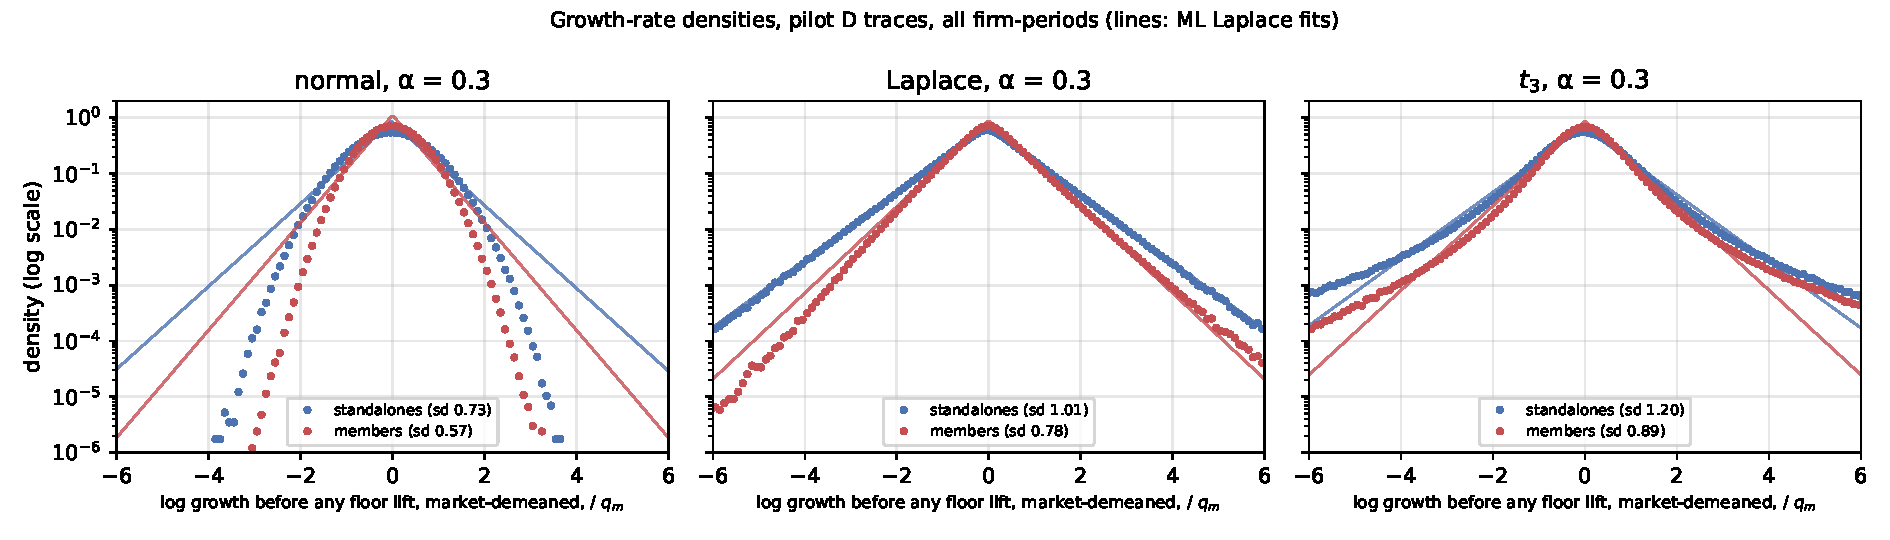
\includegraphics[width=\linewidth]{figures/appendix/growth_density_alpha0.3.pdf}
\caption{Densities of normalized per-period growth rates of members and standalones at $\alpha = 0.3$, log axis, with maximum-likelihood Laplace fits; one panel per family. 27 traced runs, moment rule.}
\label{fig:growth_density}
\end{figure}

\subsection{Concentration and rank mobility}\label{app:A17}

Table~\ref{tab:a18_concentration} gives the concentration measures behind Section~\ref{sec:results-distribution}. Within markets firms become more equal: the within-market Herfindahl index falls from 0.175--0.20 at $\alpha = 0$ to 0.14--0.17 at $\alpha = 0.3$ and 0.11--0.14 at $\alpha = 0.5$. Across the economy the units that own them become fewer and larger: the capital held by the largest ten per cent of owners, a conglomerate counted as one owner, goes from 0.65 to 0.65 (normal, with 0.67 at $\alpha = 0.3$), 0.66 to 0.74 (Laplace) and 0.68 to 0.79 ($t_3$) between $\alpha = 0$ and $0.5$; beyond $0.5$ it falls to 0.53 (normal) and 0.67 (Laplace) at $\alpha = 0.9$ while $t_3$ reaches 0.81, as the units' members grow more equal in size ($K_{\text{eff}}/K$ rises again to 0.68--0.71). Units sort by volatility and grow unequal: assortativity, the dispersion of members' market volatilities relative to that of a random set of the same size, falls from 0.60--0.61 at $\alpha = 0.01$ to 0.35--0.36 at $\alpha = 0.5$, because the consent test selects partners whose fluctuations are worth sharing from both sides; the effective number of members falls from 0.83--0.88 of $K$ to 0.64--0.68 over the same range as units accumulate a few large members and many recruits from the floor.

Tables~\ref{tab:a17_rank_mobility} and \ref{tab:a17b_rank_mobility_status} measure rank mobility from the 27 traced runs and nine traced $\alpha = 0$ runs: within each market, ranks of log share at an origin every 100 periods and 100 periods later, giving the Spearman correlation, the persistence of the top and bottom decile, leader turnover and the mean absolute rank change; a hit-free sample drops firms lifted at the floor in between and re-ranks the rest; the same by status at the origin; and the same for owning units across the economy. Pooling lowers rank mobility within markets in every family (lag-100 Spearman 0.16--0.33 at $\alpha = 0$ against 0.25--0.45 at $\alpha = 0.3$; top-decile persistence 0.31--0.48 against 0.36--0.53), partly through fewer floor lifts (0.68--0.83 of firms lifted within 100 periods against 0.52--0.71) and partly through slower movement among going concerns (members' ranks move 9--20\% less than standalones'); and it makes the top decile of owners markedly more persistent (0.32--0.49 against 0.67--0.69). Mobility is high in every cell and ranks are nearly independent at lag 500. The per-firm rank range and rank standard deviation of the earlier draft, recomputed on the traces, are at their ceiling in the floored economy and move the same way.

\begin{table}[htbp]
\centering
\caption{Concentration within markets and across owners}
\label{tab:a18_concentration}
\small
\begin{tabular}{lrrrrr}
\toprule
Family & $\alpha$ & \makecell[b]{HHI within\\{}markets} & \makecell[b]{Top-decile\\{}owners' share} & $K_{\text{eff}}/K$ & Assortativity \\
\midrule
normal & 0 & 0.175 & 0.65 & -- & -- \\
 & 0.1 & 0.164 & 0.67 & 0.75 & 0.49 \\
 & 0.3 & 0.139 & 0.67 & 0.68 & 0.39 \\
 & 0.5 & 0.109 & 0.65 & 0.65 & 0.36 \\
Laplace & 0 & 0.179 & 0.66 & -- & -- \\
 & 0.1 & 0.168 & 0.72 & 0.73 & 0.49 \\
 & 0.3 & 0.144 & 0.73 & 0.68 & 0.40 \\
 & 0.5 & 0.113 & 0.74 & 0.64 & 0.35 \\
$t_3$ & 0 & 0.201 & 0.68 & -- & -- \\
 & 0.1 & 0.191 & 0.74 & 0.74 & 0.52 \\
 & 0.3 & 0.167 & 0.77 & 0.70 & 0.42 \\
 & 0.5 & 0.136 & 0.79 & 0.67 & 0.35 \\
\bottomrule
\end{tabular}
\end{table}

\begin{sidewaystable}[htbp]
\centering
\caption{Rank mobility within markets and persistence of owners, lag 100 periods}
\label{tab:a17_rank_mobility}
\small
\begin{tabular}{lrrrrrrrr}
\toprule
Family & $\alpha$ & \makecell[b]{Spearman\\{}(all /\\{}hit-free)} & \makecell[b]{Top-decile\\{}persistence\\{}(all / hit-free)} & \makecell[b]{Leader\\{}turnover\\{}(all / hit-free)} & \makecell[b]{Mean\\{}rank\\{}change} & \makecell[b]{Share\\{}lifted\\{}within 100} & \makecell[b]{Owners:\\{}Spearman} & \makecell[b]{Owners:\\{}top-decile\\{}persistence} \\
\midrule
normal & 0 & 0.33 / 0.41 & 0.48 / 0.45 & 0.60 / 0.62 & 13.1 & 0.68 & 0.33 & 0.49 \\
 & 0.05 & 0.34 / 0.42 & 0.48 / 0.46 & 0.59 / 0.62 & 12.9 & 0.66 & 0.38 & 0.63 \\
 & 0.1 & 0.36 / 0.43 & 0.49 / 0.47 & 0.59 / 0.62 & 12.7 & 0.63 & 0.38 & 0.66 \\
 & 0.3 & 0.45 / 0.49 & 0.53 / 0.50 & 0.58 / 0.59 & 11.6 & 0.52 & 0.40 & 0.69 \\
Laplace & 0 & 0.21 / 0.31 & 0.35 / 0.36 & 0.73 / 0.71 & 14.4 & 0.78 & 0.20 & 0.37 \\
 & 0.05 & 0.22 / 0.31 & 0.36 / 0.35 & 0.73 / 0.71 & 14.3 & 0.77 & 0.24 & 0.55 \\
 & 0.1 & 0.24 / 0.32 & 0.37 / 0.35 & 0.72 / 0.72 & 14.1 & 0.75 & 0.24 & 0.59 \\
 & 0.3 & 0.32 / 0.35 & 0.41 / 0.37 & 0.71 / 0.71 & 13.2 & 0.64 & 0.27 & 0.68 \\
$t_3$ & 0 & 0.16 / 0.29 & 0.31 / 0.32 & 0.77 / 0.74 & 14.9 & 0.83 & 0.16 & 0.32 \\
 & 0.05 & 0.17 / 0.29 & 0.32 / 0.32 & 0.77 / 0.74 & 14.8 & 0.81 & 0.19 & 0.50 \\
 & 0.1 & 0.19 / 0.29 & 0.32 / 0.32 & 0.77 / 0.73 & 14.7 & 0.80 & 0.19 & 0.55 \\
 & 0.3 & 0.25 / 0.32 & 0.36 / 0.36 & 0.75 / 0.72 & 13.9 & 0.71 & 0.23 & 0.67 \\
\bottomrule
\end{tabular}
\par\smallskip\begin{minipage}{0.95\linewidth}\footnotesize Pooling lowers rank mobility within markets in every family (persistence rises with the sharing rate) and makes the top decile of owners more persistent; the hit-free columns show that part, not all, of the fall is fewer recapitalizations at the floor.\end{minipage}
\end{sidewaystable}

\begin{sidewaystable}[htbp]
\centering
\caption{Rank mobility by status at the origin, lag 100 periods}
\label{tab:a17b_rank_mobility_status}
\small
\begin{tabular}{lrrrrr}
\toprule
Family & $\alpha$ & \makecell[b]{Top-decile persistence\\{}(member / standalone)} & \makecell[b]{Mean rank change\\{}(member / standalone)} & \makecell[b]{Share lifted within 100\\{}(member / standalone)} & \makecell[b]{Members' share\\{}of the top decile} \\
\midrule
normal & 0.05 & 0.46 / 0.65 & 12.2 / 14.0 & 0.55 / 0.83 & 0.87 \\
 & 0.1 & 0.48 / 0.63 & 12.0 / 14.1 & 0.52 / 0.84 & 0.94 \\
 & 0.3 & 0.53 / 0.48 & 10.9 / 13.6 & 0.41 / 0.82 & 0.99 \\
Laplace & 0.05 & 0.35 / 0.43 & 13.6 / 15.1 & 0.67 / 0.88 & 0.88 \\
 & 0.1 & 0.37 / 0.36 & 13.4 / 15.1 & 0.65 / 0.89 & 0.93 \\
 & 0.3 & 0.41 / 0.30 & 12.5 / 14.9 & 0.54 / 0.87 & 0.97 \\
$t_3$ & 0.05 & 0.31 / 0.34 & 14.2 / 15.5 & 0.73 / 0.90 & 0.84 \\
 & 0.1 & 0.33 / 0.29 & 14.0 / 15.6 & 0.70 / 0.91 & 0.89 \\
 & 0.3 & 0.37 / 0.28 & 13.1 / 15.3 & 0.60 / 0.89 & 0.95 \\
\bottomrule
\end{tabular}
\par\smallskip\begin{minipage}{0.95\linewidth}\footnotesize Members' ranks move less than standalones' in every cell; the standalone top-decile figures rest on few firms, since members hold 84--99\% of the top decile.\end{minipage}
\end{sidewaystable}


\subsection{Scope without consent: the accept rule}\label{app:accept}

Under the accept rule every feasible proposal merges and no one leaves by choice; everything else is unchanged. It is a control without knowledge, not a behavioural alternative: it shows the scope the floor and the one-firm-per-market constraint alone permit. Table~\ref{tab:a19_accept} sets it beside the moment and loggain rules on the main power-law cells (45 runs on the main cells' seeds): $K_{\text{accept}}$ is 12.4--28.2 against 3.5--7.7, above the equal-members reference in every normal and Laplace cell and below it under $t_3$ (0.3--0.6 of $K^*$). The extra mergers are solo entries of floor-sized firms into existing units (86--89\% of the control's entries are at the floor); unit--unit mergers do not rise with consent off, because consolidated units occupy most markets and clash. The pooled share rises by 0.02--0.11, the Hill exponent by 0.00--0.04, the within-market Herfindahl index falls by 0.004--0.012, and the members' floor-hit rate rises slightly. Table~\ref{tab:decomposition-accept} is the four-part re-cut of Table~\ref{tab:decomposition} that separates what the environment permits from what consent withholds.

\begin{sidewaystable}[htbp]
\centering
\caption{The accept rule against the moment and loggain rules}
\label{tab:a19_accept}
\small
\begin{tabular}{lrrrrrrrrrr}
\toprule
Family & $\alpha$ & \makecell[b]{K:\\{}accept} & moment & loggain & \makecell[b]{Pooled:\\{}accept} & moment & \makecell[b]{Hill:\\{}accept} & moment & \makecell[b]{HHI within:\\{}accept} & moment \\
\midrule
normal & 0.1 & 17.6 & 3.7 & 3.0 & 0.95 & 0.85 & 1.12 & 1.11 & 0.160 & 0.164 \\
 & 0.3 & 22.2 & 5.5 & 4.3 & 0.97 & 0.94 & 1.21 & 1.21 & 0.133 & 0.139 \\
 & 0.5 & 28.2 & 7.7 & 6.3 & 0.98 & 0.96 & 1.37 & 1.34 & 0.106 & 0.109 \\
Laplace & 0.1 & 13.8 & 3.7 & 3.0 & 0.93 & 0.85 & 1.11 & 1.11 & 0.164 & 0.168 \\
 & 0.3 & 18.1 & 5.4 & 4.0 & 0.95 & 0.91 & 1.23 & 1.19 & 0.135 & 0.144 \\
 & 0.5 & 24.3 & 7.8 & 5.9 & 0.97 & 0.93 & 1.35 & 1.34 & 0.109 & 0.113 \\
$t_3$ & 0.1 & 12.4 & 3.5 & 2.9 & 0.91 & 0.83 & 1.04 & 1.03 & 0.188 & 0.191 \\
 & 0.3 & 16.2 & 4.8 & 3.7 & 0.94 & 0.90 & 1.13 & 1.12 & 0.160 & 0.167 \\
 & 0.5 & 21.8 & 6.8 & 5.1 & 0.96 & 0.92 & 1.26 & 1.22 & 0.127 & 0.136 \\
\bottomrule
\end{tabular}
\end{sidewaystable}

\begin{sidewaystable}[htbp]
\centering
\caption{Four-part decomposition of the distance to the equal-members reference, power-law cost; medians over five replications}
\label{tab:decomposition-accept}
\small
\begin{tabular}{lrrrrrrrrrr}
\toprule
Family & $\alpha$ & $K^*$ & $K_{\text{accept}}$ & $K_{\text{hom}}$ & $K$ & $K_{\text{loggain}}$ & Environment & Consent & Transfer & Verifiability \\
\midrule
normal & 0.1 & 8 & 17.6 & 3.8 & 3.7 & 3.0 & -9.6 (-194\%) & 13.8 (279\%) & 0.1 (2\%) & 0.6 (13\%) \\
 & 0.3 & 12 & 22.2 & 5.6 & 5.5 & 4.3 & -10.2 (-133\%) & 16.7 (216\%) & 0.1 (1\%) & 1.2 (15\%) \\
 & 0.5 & 13 & 28.2 & 8.0 & 7.7 & 6.3 & -15.2 (-228\%) & 20.2 (304\%) & 0.3 (4\%) & 1.4 (20\%) \\
\midrule
Laplace & 0.1 & 10 & 13.8 & 3.8 & 3.7 & 3.0 & -3.8 (-55\%) & 10.0 (143\%) & 0.1 (1\%) & 0.7 (10\%) \\
 & 0.3 & 16 & 18.1 & 5.5 & 5.4 & 4.0 & -2.1 (-18\%) & 12.6 (105\%) & 0.1 (1\%) & 1.4 (12\%) \\
 & 0.5 & 20 & 24.3 & 8.2 & 7.8 & 5.9 & -4.3 (-31\%) & 16.1 (115\%) & 0.4 (3\%) & 1.8 (13\%) \\
\midrule
$t_3$ & 0.1 & 20 & 12.4 & 3.5 & 3.5 & 2.9 & 7.6 (44\%) & 8.9 (52\%) & 0.0 (0\%) & 0.6 (4\%) \\
 & 0.3 & 47 & 16.2 & 4.9 & 4.8 & 3.7 & 30.8 (71\%) & 11.3 (26\%) & 0.1 (0\%) & 1.2 (3\%) \\
 & 0.5 & 50 & 21.8 & 7.0 & 6.8 & 5.1 & 28.2 (63\%) & 14.8 (33\%) & 0.2 (0\%) & 1.7 (4\%) \\
\bottomrule
\end{tabular}
\par\smallskip\begin{minipage}{0.95\linewidth}\footnotesize Environment $= K^* - K_{\text{accept}}$, consent $= K_{\text{accept}} - K_{\text{hom}}$, transfer $= K_{\text{hom}} - K$, verifiability $= K - K_{\text{loggain}}$; shares in parentheses are of $K^* - K_{\text{loggain}}$ (the four parts sum to it). $K_{\text{accept}}$: heterogeneous economy, every feasible proposal accepted and no voluntary exit (a control without knowledge). A negative environment part means the environment alone permits units larger than $K^*$. The consent part compares the heterogeneous accept economy with the homogeneous moment economy, so it also holds the homogeneous-heterogeneous difference of the accept rule.\end{minipage}
\end{sidewaystable}


\subsection{The sharing rate}\label{app:alpha}

Table~\ref{tab:endogenous} gives the endogenous-$\alpha$ block under the power-law cost and Table~\ref{tab:a13_endogenous} under all four cost forms and both rules. Units that choose their rate reach 14--18 mean members under the power-law cost, with 95--98\% of capital pooled and a tail exponent of 1.8--2.1. This is the scope that a rate near 0.9 implies, not a separate effect: along the fixed-rate grid $K$ rises from 5.4 at $\alpha = 0.3$ to 7.8 at $0.5$, and the fixed $\alpha = 0.9$ cell reproduces the endogenous block (Table~\ref{tab:robustness-b}). The ordering across families is the same as elsewhere: the heaviest tails choose a slightly lower rate and reach a smaller scope. The exponential-cost cells reach $K = 16$--23 at a lower pooled share (81--92\%). Neither heterogeneity among members nor the volatility of their markets drives the choice: across 7,630 units active at the end of a run, the Spearman correlation of a unit's time-averaged rate with the dispersion of its members' volatilities is $-0.14$ to $0.00$, and with their mean volatility 0.04--0.10. Under the loggain rule the latter was 0.14--0.26: units in more volatile markets pooled more, not because the optimum differed, it is full pooling at every volatility level, but because only there was the gain from a higher rate large enough to show through the window's noise.

\begin{table}[htbp]
\centering
\caption{The sharing rate units choose}
\label{tab:endogenous}
\small
\begin{tabular}{lrrrrrrr}
\toprule
Family & $\bar\alpha$ & median & share at 1 & $K$ & Pooled & Hill & $\rho(\alpha, \bar q)$ \\
\midrule
normal & 0.93 & 0.90 & 0.22 & 16.9 & 0.98 & 2.05 & 0.10 \\
Laplace & 0.92 & 0.90 & 0.14 & 18.0 & 0.97 & 2.07 & 0.05 \\
$t_3$ & 0.91 & 0.90 & 0.12 & 14.3 & 0.95 & 1.83 & 0.04 \\
\bottomrule
\end{tabular}
\par\smallskip\begin{minipage}{0.95\linewidth}\footnotesize Endogenous-$\alpha$ block, power-law cost, start $\alpha_C = 0.1$; adopted $\alpha$ over unit-periods; share at 1: unit-periods at $\alpha_C = 1$. $\rho$: Spearman correlation of a unit's time-averaged rate with the mean IQR of its members' markets, over the 2,468 / 2,319 / 2,843 units alive at $T$ (normal / Laplace / $t_3$). For comparison, the fixed $\alpha = 0.9$ cell gives $K = 16.0$, Hill 1.98; $K = 17.2$, Hill 1.94; $K = 13.9$, Hill 1.78 (same order).\end{minipage}
\end{table}

\begin{sidewaystable}[htbp]
\centering
\caption{Endogenous $\alpha$ by cost form}
\label{tab:a13_endogenous}
\small
\begin{tabular}{lrrrrrrr}
\toprule
Family & Cost form & $\bar\alpha$ & \makecell[b]{median,\\{}moment / loggain} & \makecell[b]{share\\{}at 1} & \makecell[b]{K,\\{}moment / loggain} & Pooled & Hill \\
\midrule
normal & power law & 0.93 & 0.90 / 0.85 & 0.22 & 16.9 / 12.1 & 0.98 & 2.05 \\
 & linear & 0.93 & 0.90 / 0.85 & 0.23 & 17.2 / 11.8 & 0.98 & 2.07 \\
 & quadratic & 0.93 & 0.90 / 0.85 & 0.20 & 17.5 / 12.6 & 0.98 & 2.02 \\
 & exponential & 0.94 & 0.95 / 0.80 & 0.24 & 23.2 / 20.5 & 0.81 & 1.88 \\
Laplace & power law & 0.92 & 0.90 / 0.80 & 0.14 & 18.0 / 11.5 & 0.97 & 2.07 \\
 & linear & 0.92 & 0.90 / 0.85 & 0.13 & 18.5 / 11.8 & 0.97 & 2.06 \\
 & quadratic & 0.93 & 0.90 / 0.80 & 0.17 & 18.8 / 12.4 & 0.97 & 2.06 \\
 & exponential & 0.93 & 0.95 / 0.85 & 0.16 & 22.1 / 16.0 & 0.91 & 2.00 \\
$t_3$ & power law & 0.91 & 0.90 / 0.80 & 0.12 & 14.3 / 8.8 & 0.95 & 1.83 \\
 & linear & 0.92 & 0.90 / 0.80 & 0.14 & 14.3 / 8.7 & 0.95 & 1.84 \\
 & quadratic & 0.91 & 0.90 / 0.80 & 0.11 & 14.4 / 9.2 & 0.95 & 1.84 \\
 & exponential & 0.91 & 0.90 / 0.80 & 0.10 & 16.0 / 10.4 & 0.92 & 1.83 \\
\bottomrule
\end{tabular}
\end{sidewaystable}


\section{Robustness}\label{app:robustness}

\subsection{Summary}

Tables~\ref{tab:robustness} and \ref{tab:robustness-b} summarize every block at $\alpha = 0.3$ (the endogenous-$\alpha$ block at its adopted rate) against the Laplace power-law baseline. The rest of this section gives each block in full.

\begin{table}[htbp]
\centering
\caption{Robustness: environment and decision parameters}
\label{tab:robustness}
\small
\begin{tabular}{llrrrr}
\toprule
Block & Variant & $K$ & Pooled & Hill & Floor exits \\
\midrule
cost form & linear & 5.2 & 0.91 & 1.18 & 35 \\
 & quadratic & 5.9 & 0.92 & 1.19 & 36 \\
 & exponential & 6.1 & 0.88 & 1.21 & 36 \\
\midrule
cost level & $\times 0.5$ & 6.0 & 0.92 & 1.20 & 35 \\
 & $\times 2$ & 4.7 & 0.91 & 1.19 & 35 \\
 & $\times 5$ & 3.9 & 0.87 & 1.17 & 33 \\
 & $\times 10$ & 3.3 & 0.79 & 1.15 & 33 \\
 & $\times 20$ & 2.8 & 0.67 & 1.13 & 33 \\
\midrule
window $l$ & 20 & 4.8 & 0.91 & 1.19 & 35 \\
 & 100 & 5.8 & 0.92 & 1.20 & 37 \\
 & 200 & 6.1 & 0.93 & 1.21 & 34 \\
 & 500 & 6.6 & 0.92 & 1.20 & 38 \\
\midrule
search $p$ & 0.2 & 6.8 & 0.97 & 1.18 & 62 \\
 & 1 & 8.0 & 0.98 & 1.18 & 116 \\
\midrule
correlation & cross-market 0.3 & 5.3 & 0.91 & 1.21 & 36 \\
\midrule
floor $c$ & 0.10 & 5.6 & 0.93 & 1.13 & 32 \\
 & 0.35 & 4.4 & 0.74 & 1.66 & 60 \\
\midrule
economy size $(M, N)$ & (25, 25) & 5.6 & 0.96 & 1.22 & 7 \\
 & (100, 25) & 6.2 & 0.96 & 1.24 & 23 \\
 & (25, 100) & 4.7 & 0.88 & 1.16 & 44 \\
 & (100, 100) & 5.2 & 0.89 & 1.17 & 170 \\
\bottomrule
\end{tabular}
\par\smallskip\begin{minipage}{0.95\linewidth}\footnotesize At $\alpha = 0.3$, Laplace shocks, power-law cost unless stated, moment rule; medians over five replications. Baseline: $K = 5.4$, pooled 0.91, Hill 1.19, 36 floor exits per period. \end{minipage}
\end{table}

\begin{table}[htbp]
\centering
\caption{Robustness: contract, shock family and decision rule}
\label{tab:robustness-b}
\small
\begin{tabular}{llrrrr}
\toprule
Block & Variant & $K$ & Pooled & Hill & Floor exits \\
\midrule
equal split (normal) & linear & 2.9 & 0.29 & 1.12 & 21 \\
 & quadratic & 3.0 & 0.33 & 1.14 & 24 \\
 & exponential & 2.8 & 0.24 & 1.09 & 21 \\
 & power law & 3.0 & 0.33 & 1.13 & 24 \\
\midrule
endogenous $\alpha$ & normal & 16.9 & 0.98 & 2.05 & 2 \\
 & Laplace & 18.0 & 0.97 & 2.07 & 4 \\
 & $t_3$ & 14.3 & 0.95 & 1.83 & 11 \\
\midrule
fixed $\alpha = 0.9$ & normal & 16.0 & 0.98 & 1.98 & 2 \\
 & Laplace & 17.2 & 0.97 & 1.94 & 5 \\
 & $t_3$ & 13.9 & 0.95 & 1.78 & 11 \\
\midrule
tail weight $\nu$ (Student-$t$) & 2.5 & 4.1 & 0.85 & 1.02 & 54 \\
 & 3 & 4.8 & 0.90 & 1.12 & 42 \\
 & 4 & 5.3 & 0.92 & 1.17 & 33 \\
\midrule
homogeneous markets & normal & 5.6 & 0.94 & 1.20 & 22 \\
 & Laplace & 5.5 & 0.91 & 1.19 & 34 \\
 & $t_3$ & 4.9 & 0.89 & 1.10 & 42 \\
\midrule
loggain rule & normal & 4.3 & 0.73 & 1.17 & 26 \\
 & Laplace & 4.0 & 0.78 & 1.16 & 37 \\
 & $t_3$ & 3.7 & 0.77 & 1.10 & 43 \\
\bottomrule
\end{tabular}
\par\smallskip\begin{minipage}{0.95\linewidth}\footnotesize Conventions as in Table~\ref{tab:robustness}; family rows are at $\alpha = 0.3$ except the endogenous-$\alpha$ block. Homogeneous markets: every market at $q = 0.20$.\end{minipage}
\end{table}


\subsection{Cost form and level}\label{app:cost}

Table~\ref{tab:a10_cost_forms} gives the four cost forms at equal $\Phi(40)$ for all three families; the form moves scope by under one member. Table~\ref{tab:costlevel} runs the power-law level from $\times 0.5$ to $\times 20$ at $\alpha = 0.3$ under both rules with the equal-members reference recomputed at each level: scope falls by about 0.6 members per doubling of the cost and the ratio $K/K^*$ rises, but the reference is never reached, because the reference falls with the cost as well. Table~\ref{tab:a10b_cost_levels} gives the $\times 0.5$ and $\times 2$ cells for every form, with $b_0$ alone scaled (power law and exponential: the whole schedule) or all coefficients scaled (linear, quadratic).

\begin{table}[htbp]
\centering
\caption{Cost forms at equal $\Phi$(40), $\alpha$ = 0.3}
\label{tab:a10_cost_forms}
\small
\begin{tabular}{lrrrrr}
\toprule
Family & Cost form & K & Pooled & Hill & Acceptance \\
\midrule
normal & power law & 5.5 & 0.94 & 1.21 & 0.29 \\
normal & linear & 5.3 & 0.93 & 1.21 & 0.26 \\
normal & quadratic & 6.4 & 0.94 & 1.22 & 0.34 \\
normal & exponential & 6.6 & 0.87 & 1.22 & 0.35 \\
Laplace & power law & 5.4 & 0.91 & 1.19 & 0.40 \\
Laplace & linear & 5.2 & 0.91 & 1.18 & 0.39 \\
Laplace & quadratic & 5.9 & 0.92 & 1.19 & 0.42 \\
Laplace & exponential & 6.1 & 0.88 & 1.21 & 0.44 \\
$t_3$ & power law & 4.8 & 0.90 & 1.12 & 0.44 \\
$t_3$ & linear & 4.6 & 0.88 & 1.10 & 0.46 \\
$t_3$ & quadratic & 4.9 & 0.88 & 1.09 & 0.49 \\
$t_3$ & exponential & 5.2 & 0.86 & 1.11 & 0.47 \\
\bottomrule
\end{tabular}
\end{table}

\begin{table}[htbp]
\centering
\caption{Cost level, power-law form, $\alpha = 0.3$; medians over five replications}
\label{tab:costlevel}
\small
\begin{tabular}{lrrrrrrrr}
\toprule
Family & Cost level & $K$ & $K$, loggain & $K^*$ & $K/K^*$ & Pooled & Accept. & Hill \\
\midrule
Laplace & 0.5 & 6.0 & 4.3 & -- & -- & 0.92 & 0.42 & 1.20 \\
 & 1 & 5.4 & 4.0 & 16 & 0.34 & 0.91 & 0.40 & 1.19 \\
 & 2 & 4.7 & 3.7 & -- & -- & 0.91 & 0.36 & 1.19 \\
 & 5 & 3.9 & 3.1 & 8 & 0.49 & 0.87 & 0.31 & 1.17 \\
 & 10 & 3.3 & 2.8 & 6 & 0.55 & 0.79 & 0.29 & 1.15 \\
 & 20 & 2.8 & 2.5 & 4 & 0.70 & 0.67 & 0.29 & 1.13 \\
\midrule
$t_3$ & 1 & 4.8 & 3.7 & 47 & 0.10 & 0.90 & 0.44 & 1.12 \\
 & 5 & 3.7 & 3.0 & 10 & 0.37 & 0.85 & 0.38 & 1.10 \\
 & 10 & 3.3 & 2.8 & 7 & 0.47 & 0.80 & 0.37 & 1.07 \\
 & 20 & 2.8 & 2.5 & 5 & 0.57 & 0.70 & 0.36 & 1.05 \\
\bottomrule
\end{tabular}
\end{table}

\begin{table}[htbp]
\centering
\caption{Cost level $\times$0.5 and $\times$2, Laplace}
\label{tab:a10b_cost_levels}
\small
\begin{tabular}{lrrrrrr}
\toprule
Scaled & Cost form & Level & $\alpha$ & K & Pooled & Acceptance \\
\midrule
$b_0$ only & exponential & $\times$0.5 & 0.1 & 4.5 & 0.75 & 0.46 \\
$b_0$ only & exponential & $\times$0.5 & 0.3 & 6.4 & 0.91 & 0.46 \\
$b_0$ only & exponential & $\times$0.5 & 0.5 & 9.5 & 0.94 & 0.44 \\
$b_0$ only & exponential & $\times$2 & 0.1 & 3.6 & 0.38 & 0.32 \\
$b_0$ only & exponential & $\times$2 & 0.3 & 5.5 & 0.81 & 0.42 \\
$b_0$ only & exponential & $\times$2 & 0.5 & 8.0 & 0.91 & 0.40 \\
$b_0$ only & linear & $\times$0.5 & 0.1 & 3.6 & 0.82 & 0.42 \\
$b_0$ only & linear & $\times$0.5 & 0.3 & 5.3 & 0.91 & 0.39 \\
$b_0$ only & linear & $\times$0.5 & 0.5 & 7.7 & 0.94 & 0.37 \\
$b_0$ only & linear & $\times$2 & 0.1 & 3.6 & 0.82 & 0.44 \\
$b_0$ only & linear & $\times$2 & 0.3 & 5.2 & 0.91 & 0.41 \\
$b_0$ only & linear & $\times$2 & 0.5 & 7.6 & 0.93 & 0.39 \\
$b_0$ only & power law & $\times$0.5 & 0.1 & 4.1 & 0.88 & 0.43 \\
$b_0$ only & power law & $\times$0.5 & 0.3 & 6.0 & 0.92 & 0.42 \\
$b_0$ only & power law & $\times$0.5 & 0.5 & 8.7 & 0.94 & 0.40 \\
$b_0$ only & power law & $\times$2 & 0.1 & 3.3 & 0.80 & 0.39 \\
$b_0$ only & power law & $\times$2 & 0.3 & 4.7 & 0.91 & 0.36 \\
$b_0$ only & power law & $\times$2 & 0.5 & 6.7 & 0.94 & 0.32 \\
$b_0$ only & quadratic & $\times$0.5 & 0.1 & 4.2 & 0.87 & 0.47 \\
$b_0$ only & quadratic & $\times$0.5 & 0.3 & 5.9 & 0.91 & 0.45 \\
$b_0$ only & quadratic & $\times$0.5 & 0.5 & 8.4 & 0.93 & 0.41 \\
$b_0$ only & quadratic & $\times$2 & 0.1 & 4.2 & 0.83 & 0.46 \\
$b_0$ only & quadratic & $\times$2 & 0.3 & 5.9 & 0.91 & 0.44 \\
$b_0$ only & quadratic & $\times$2 & 0.5 & 8.3 & 0.94 & 0.41 \\
all coefficients & linear & $\times$0.5 & 0.1 & 4.0 & 0.87 & 0.44 \\
all coefficients & linear & $\times$0.5 & 0.3 & 6.0 & 0.92 & 0.42 \\
all coefficients & linear & $\times$0.5 & 0.5 & 8.9 & 0.94 & 0.40 \\
all coefficients & linear & $\times$2 & 0.1 & 3.2 & 0.75 & 0.40 \\
all coefficients & linear & $\times$2 & 0.3 & 4.6 & 0.90 & 0.35 \\
all coefficients & linear & $\times$2 & 0.5 & 6.6 & 0.93 & 0.32 \\
all coefficients & quadratic & $\times$0.5 & 0.1 & 4.5 & 0.88 & 0.48 \\
all coefficients & quadratic & $\times$0.5 & 0.3 & 6.3 & 0.92 & 0.46 \\
all coefficients & quadratic & $\times$0.5 & 0.5 & 9.1 & 0.94 & 0.43 \\
all coefficients & quadratic & $\times$2 & 0.1 & 3.9 & 0.81 & 0.44 \\
all coefficients & quadratic & $\times$2 & 0.3 & 5.4 & 0.91 & 0.41 \\
all coefficients & quadratic & $\times$2 & 0.5 & 7.6 & 0.93 & 0.37 \\
\bottomrule
\end{tabular}
\end{table}


\subsection{Floor level, correlation and economy size}\label{app:environment}

Tables~\ref{tab:a11a_floor}--\ref{tab:a11c_size}, Laplace shocks and power-law cost. The floor level sets the tail exponent and little else: scope moves by $+3\%$ at $c = 0.10$ and $-19\%$ at $c = 0.35$ while the Hill exponent moves from 1.13 to 1.66 at $\alpha = 0.3$. Cross-market correlation of 0.3 leaves every outcome within 0.2 of the baseline. Economy size matters through the number of firms per market and barely through the number of markets, with the floor recalibrated to $c^*(N)$.

\begin{table}[htbp]
\centering
\caption{Floor level}
\label{tab:a11a_floor}
\small
\begin{tabular}{lrrrrrr}
\toprule
c & $\alpha$ & K & Pooled & Hill & Acceptance & \makecell[b]{Floor exits\\{}/ period} \\
\midrule
0.1 & 0.1 & 3.8 & 0.87 & 1.05 & 0.38 & 42.3 \\
0.1 & 0.3 & 5.6 & 0.93 & 1.13 & 0.36 & 31.5 \\
0.1 & 0.5 & 8.2 & 0.95 & 1.29 & 0.34 & 20.3 \\
0.35 & 0.1 & 3.3 & 0.68 & 1.55 & 0.60 & 69.9 \\
0.35 & 0.3 & 4.4 & 0.74 & 1.66 & 0.56 & 59.9 \\
0.35 & 0.5 & 5.8 & 0.78 & 1.80 & 0.53 & 47.7 \\
\bottomrule
\end{tabular}
\end{table}

\begin{table}[htbp]
\centering
\caption{Cross-market correlation 0.3}
\label{tab:a11b_correlation}
\small
\begin{tabular}{lrrrrrr}
\toprule
correlation & $\alpha$ & K & Pooled & Hill & Acceptance & \makecell[b]{Floor exits\\{}/ period} \\
\midrule
0.3 & 0.1 & 3.7 & 0.85 & 1.10 & 0.42 & 47.1 \\
0.3 & 0.3 & 5.3 & 0.91 & 1.21 & 0.40 & 36.3 \\
0.3 & 0.5 & 7.6 & 0.94 & 1.34 & 0.37 & 24.3 \\
\bottomrule
\end{tabular}
\end{table}

\begin{table}[htbp]
\centering
\caption{Economy size with $c^*$(N)}
\label{tab:a11c_size}
\small
\begin{tabular}{lrrrrrr}
\toprule
M / N & $\alpha$ & K & Pooled & Hill & Acceptance & \makecell[b]{Floor exits\\{}/ period} \\
\midrule
25 / 25 & 0.1 & 3.8 & 0.91 & 1.13 & 0.38 & 9.0 \\
25 / 25 & 0.3 & 5.6 & 0.96 & 1.22 & 0.40 & 6.5 \\
25 / 25 & 0.5 & 8.0 & 0.97 & 1.45 & 0.39 & 3.9 \\
25 / 100 & 0.1 & 3.5 & 0.81 & 1.10 & 0.52 & 53.9 \\
25 / 100 & 0.3 & 4.7 & 0.88 & 1.16 & 0.52 & 43.7 \\
25 / 100 & 0.5 & 6.3 & 0.91 & 1.26 & 0.50 & 31.1 \\
100 / 25 & 0.1 & 4.0 & 0.91 & 1.12 & 0.29 & 33.3 \\
100 / 25 & 0.3 & 6.2 & 0.96 & 1.24 & 0.24 & 23.1 \\
100 / 25 & 0.5 & 9.4 & 0.97 & 1.45 & 0.20 & 13.0 \\
100 / 100 & 0.1 & 3.6 & 0.82 & 1.09 & 0.46 & 215.9 \\
100 / 100 & 0.3 & 5.2 & 0.89 & 1.17 & 0.40 & 170.2 \\
100 / 100 & 0.5 & 7.6 & 0.91 & 1.28 & 0.35 & 118.3 \\
\bottomrule
\end{tabular}
\end{table}


\subsection{Homogeneous markets}\label{app:homogeneous}

Table~\ref{tab:a8_homogeneous}: every market at $q = 0.20$, power-law cost, both rules. The homogeneous economy is the $K_{\text{hom}}$ of Table~\ref{tab:decomposition}; it exceeds the heterogeneous base case by 0.0--0.4 members, which bounds the transfer conflict between members of unequal volatility.

\begin{table}[htbp]
\centering
\caption{Homogeneous block}
\label{tab:a8_homogeneous}
\small
\begin{tabular}{lrrrrrr}
\toprule
Family & Rule & $\alpha$ & K & Pooled & Acceptance & Hill \\
\midrule
normal & moment & 0.05 & 3.2 & 0.77 & 0.30 & 1.09 \\
normal & moment & 0.1 & 3.8 & 0.86 & 0.29 & 1.10 \\
normal & moment & 0.3 & 5.6 & 0.94 & 0.26 & 1.20 \\
normal & moment & 0.5 & 8.0 & 0.96 & 0.23 & 1.34 \\
normal & loggain & 0.05 & 2.8 & 0.49 & 0.32 & 1.07 \\
normal & loggain & 0.1 & 3.2 & 0.58 & 0.32 & 1.08 \\
normal & loggain & 0.3 & 4.6 & 0.75 & 0.26 & 1.18 \\
normal & loggain & 0.5 & 6.8 & 0.93 & 0.22 & 1.33 \\
Laplace & moment & 0.05 & 3.3 & 0.80 & 0.42 & 1.07 \\
Laplace & moment & 0.1 & 3.8 & 0.86 & 0.41 & 1.10 \\
Laplace & moment & 0.3 & 5.5 & 0.91 & 0.38 & 1.19 \\
Laplace & moment & 0.5 & 8.2 & 0.93 & 0.35 & 1.33 \\
Laplace & loggain & 0.05 & 2.8 & 0.57 & 0.42 & 1.07 \\
Laplace & loggain & 0.1 & 3.1 & 0.64 & 0.41 & 1.09 \\
Laplace & loggain & 0.3 & 4.2 & 0.80 & 0.35 & 1.17 \\
Laplace & loggain & 0.5 & 6.3 & 0.91 & 0.31 & 1.32 \\
$t_3$ & moment & 0.05 & 3.1 & 0.77 & 0.47 & 1.01 \\
$t_3$ & moment & 0.1 & 3.5 & 0.83 & 0.46 & 1.02 \\
$t_3$ & moment & 0.3 & 4.9 & 0.89 & 0.43 & 1.10 \\
$t_3$ & moment & 0.5 & 7.0 & 0.92 & 0.39 & 1.22 \\
$t_3$ & loggain & 0.05 & 2.7 & 0.57 & 0.46 & 1.00 \\
$t_3$ & loggain & 0.1 & 2.9 & 0.64 & 0.45 & 1.01 \\
$t_3$ & loggain & 0.3 & 3.8 & 0.79 & 0.40 & 1.08 \\
$t_3$ & loggain & 0.5 & 5.3 & 0.89 & 0.35 & 1.20 \\
\bottomrule
\end{tabular}
\end{table}


\subsection{Tail weight}\label{app:nu}

Table~\ref{tab:a9_nu}: Student-$t$ shocks with $\nu \in \{2.5, 3, 4\}$ at equal IQR, power-law cost, moment rule. The last two columns give the distribution of the window variance estimate relative to its population value over 200,000 i.i.d.\ 50-period windows at $q = 0.2$, and the share of windows in which it is below one half. Scope falls with tail weight while acceptance rises: under heavier tails firms are more willing to pool and less able to stay pooled, because members are recapitalized more often. Attrition, not consent, takes the scope.

\begin{sidewaystable}[htbp]
\centering
\caption{$\nu$ block}
\label{tab:a9_nu}
\small
\begin{tabular}{lrrrrrrrrr}
\toprule
$\nu$ & $\alpha$ & K & Pooled & Hill & Acceptance & \makecell[b]{Floor exits\\{}/ period} & \makecell[b]{Hazard\\{}ratio} & \makecell[b]{$\hat\sigma^2/\sigma^2$\\{}median [5\%, 95\%]} & \makecell[b]{share\\{}< $\tfrac12$} \\
\midrule
2.5 & 0.1 & 3.2 & 0.78 & 0.96 & 0.54 & 63.3 & 0.25 & 0.59 [0.29, 2.01] & 0.37 \\
 & 0.3 & 4.1 & 0.85 & 1.02 & 0.50 & 53.5 & 0.17 &  &  \\
 & 0.5 & 5.5 & 0.88 & 1.12 & 0.46 & 42.0 & 0.12 &  &  \\
3 & 0.1 & 3.5 & 0.83 & 1.03 & 0.47 & 53.1 & 0.19 & 0.77 [0.42, 1.98] & 0.13 \\
 & 0.3 & 4.8 & 0.90 & 1.12 & 0.44 & 42.5 & 0.13 &  &  \\
 & 0.5 & 6.8 & 0.92 & 1.22 & 0.41 & 31.2 & 0.08 &  &  \\
4 & 0.1 & 3.7 & 0.85 & 1.07 & 0.39 & 43.7 & 0.15 & 0.89 [0.53, 1.74] & 0.03 \\
 & 0.3 & 5.3 & 0.92 & 1.17 & 0.37 & 33.4 & 0.10 &  &  \\
 & 0.5 & 7.7 & 0.94 & 1.31 & 0.34 & 21.8 & 0.06 &  &  \\
\bottomrule
\end{tabular}
\end{sidewaystable}


\subsection{Equal sharing}\label{app:equalsplit}

Table~\ref{tab:a12_equal_split}: equal dollar splits of the net pool, normal shocks, four cost forms, with acceptance by proposal type (standalone--standalone, standalone--unit), voluntary exits, pool ruin (a unit's members capped at limited liability in a period) and the shortfall charged to the other members. Mean scope is 2.1--3.2 at every sharing rate and pooled capital never exceeds 34\%, against 3.2--7.7 and up to 96\% under proportional sharing. The reason is visible in who consents: proposals between two unaffiliated firms pass at 3--48\% under equal sharing against 95--100\% under proportional, proposals of a standalone to a unit at 6--17\% against 28--41\%. Under an equal split the larger partner subsidizes the smaller in every period in which it does better, which it expects to do half the time, and refuses. The contract decides whether conglomerates exist at all.

\begin{sidewaystable}[htbp]
\centering
\caption{Equal-split block}
\label{tab:a12_equal_split}
\small
\begin{tabular}{lrrrrrrrr}
\toprule
Cost form & $\alpha$ & K & Pooled & \makecell[b]{Acceptance\\{}s--s} & \makecell[b]{Acceptance\\{}s--u} & \makecell[b]{Voluntary\\{}exits / period} & \makecell[b]{Pool ruin\\{}/ period} & \makecell[b]{Shortfall\\{}/ period} \\
\midrule
exponential & 0.05 & 2.2 & 0.03 & 0.03 & 0.06 & 0.5 & 0.000 & 0.0e+00 \\
 & 0.1 & 2.5 & 0.14 & 0.16 & 0.13 & 2.4 & 0.001 & 7.1e-06 \\
 & 0.3 & 2.8 & 0.24 & 0.30 & 0.14 & 4.0 & 0.010 & 5.6e-04 \\
 & 0.5 & 2.9 & 0.25 & 0.29 & 0.13 & 4.7 & 0.029 & 2.5e-03 \\
linear & 0.05 & 2.5 & 0.26 & 0.39 & 0.15 & 3.3 & 0.000 & 0.0e+00 \\
 & 0.1 & 2.6 & 0.28 & 0.41 & 0.15 & 3.5 & 0.001 & 1.4e-05 \\
 & 0.3 & 2.9 & 0.29 & 0.37 & 0.14 & 4.2 & 0.012 & 7.4e-04 \\
 & 0.5 & 3.0 & 0.29 & 0.33 & 0.13 & 4.8 & 0.039 & 3.2e-03 \\
power law & 0.05 & 2.6 & 0.31 & 0.48 & 0.17 & 3.1 & 0.000 & 0.0e+00 \\
 & 0.1 & 2.7 & 0.32 & 0.48 & 0.17 & 3.3 & 0.001 & 3.3e-05 \\
 & 0.3 & 3.0 & 0.33 & 0.43 & 0.16 & 3.9 & 0.017 & 1.2e-03 \\
 & 0.5 & 3.1 & 0.33 & 0.38 & 0.14 & 4.6 & 0.050 & 3.9e-03 \\
quadratic & 0.05 & 2.7 & 0.29 & 0.45 & 0.17 & 3.2 & 0.000 & 0.0e+00 \\
 & 0.1 & 2.7 & 0.31 & 0.46 & 0.17 & 3.3 & 0.001 & 2.6e-05 \\
 & 0.3 & 3.0 & 0.33 & 0.43 & 0.16 & 4.0 & 0.016 & 8.9e-04 \\
 & 0.5 & 3.1 & 0.33 & 0.37 & 0.14 & 4.6 & 0.046 & 3.8e-03 \\
\bottomrule
\end{tabular}
\end{sidewaystable}


\section{Computation}\label{app:computation}

\subsection{Identity protocol and tests}\label{app:identity}

Every change to the code after the model was frozen (the diagnostics, the limited-liability correction, the counters, the moment rule, the production block and the traced runs) was accompanied by an identity check: every scenario whose behaviour the change should not touch is rerun on the new code and its result and summary row compared byte for byte with the stored ones, excluding runtime fields and new keys. The production block passes 1,995 of 1,995 scenarios and the accept-rule addition 2,055 of 2,055; the loggain reference block is frozen and verified by checksum. The test suite (281 tests) covers the pooling identity under limited liability (unit capital after pooling equals the sum of members' gross returns net of the coordination cost, to $10^{-9}$), the moment rule against hand-computed cases and against the loggain replay on long windows, the kernel counters' sums, the design counts and the summary schema. Three pool wipeouts (every member of a unit at the floor in the same period) occurred in 1,995 runs, one event each; they are counted, not asserted away.

\subsection{Files and provenance}\label{app:files}

The repository holds the simulation code, the design files, the per-run summaries of the production block and the loggain reference block, the traced runs' panels and every derived file behind a table or figure; \texttt{analysis/paper\_tables.py}, \texttt{analysis/paper\_figures.py} and \texttt{analysis/appendix\_tables.py} regenerate every exhibit from them. The commit the paper is frozen on and the archive DOI are given in the code and data availability statement.
 after the main text and before the bibliography.
% Needs in the preamble: \usepackage{booktabs,makecell,rotating} (algorithm2e, amsmath, graphicx are already loaded).
% Every table is generated: latex/tables/*.tex by analysis/paper_tables.py (the tables moved out of Section 4),
% latex/tables/appendix/*.tex by analysis/appendix_tables.py; nothing in a table is typed.
% Labels used by the main text: app:A6 (recruit size), app:A17 (rank mobility), alg:period (Section 3.3).
% Suggested split if the journal's printed length is tight: A and B printed, C and D as an online supplement.
% ---------------------------------------------------------------------------------------------------------------
\appendix
\numberwithin{table}{section}
\numberwithin{figure}{section}
\renewcommand{\thetable}{\thesection\arabic{table}}
\renewcommand{\thefigure}{\thesection\arabic{figure}}

\section{Model details and benchmarks}\label{app:model}

\subsection{Order of events within a period}\label{app:algorithm}

Algorithm~\ref{alg:period} gives the order of events within a period. Merger and exit decisions use the window $\{t-l, \dots, t-1\}$; the current period's shock is never part of the information on which a decision is taken, and a unit formed in period $t$ pools from period $t$ on.

\begin{algorithm}[H]
\caption{Order of events within a period}\label{alg:period}
\SetAlgoLined
Draw $x_{it}$ for all firms; compute $G_{mt}$ and $\tilde r_{it}$\;
[endogenous-$\alpha$ block] every unit renegotiates $\alpha_C$ on the grid over the last $l$ periods: unanimity first, maximin second\;
\ForEach{firm $i$ drawn as initiator with probability $p$}{
  draw a target market among those its unit does not occupy and a target firm in it\;
  \If{the merged set has at most one firm per market and $\tilde\Delta_i(\hat C, \alpha) > \max\{0, \tilde\Delta_i(C_i, \alpha)\}$ for every member}{
    merge; set the entry period of every new member (of every member if two units merge) to $t$\;
  }
}
\ForEach{conglomerate}{
  $\delta_{jt}$ for each member by the pooling equation; a member whose factor would fall below zero keeps nothing and its shortfall is charged to the other members pro rata to their post-pooling capital\;
}
$s_{i,t+1} = s_{it}\,\delta_{it}$ for members, $s_{it}\,e^{\tilde r_{it}}$ for unaffiliated firms\;
\ForEach{market}{
  lift every firm below $c \times$ mean size to that level, iterating to the fixed point; count floor hits; a lifted member leaves its unit; renormalize the market to mean size one\;
}
\ForEach{member with tenure $> l$}{
  leave if $\tilde\Delta_i(C_i, \alpha) < 0$\;
}
dissolve units with one member\;
every 100 periods: record the size distribution, membership and unit capital\;
\end{algorithm}

Two details of the floor. Since sizes are shares of a market whose capital is the numeraire, an entrant's share dilutes the incumbents' shares in proportion to their size, as any entry does; after pooling and the floor every market is renormalized to mean size one, which is where this dilution takes place. What survives the loss of the firm's capital is the configuration's knowledge, whether as the same firm recapitalized or as a start-up formed by its people, and with it its record.

\subsection{The equal-members reference}\label{app:kstar}

$K^*$ is the scope that maximizes the time-average growth of a member in a unit of equal members facing i.i.d.\ shocks at the median market volatility $q = 0.20$, net of the coordination cost. It is computed by Monte Carlo ($2 \times 10^6$ draws per $K$) and capped at $M = 50$. Table~\ref{tab:a1_kstar} gives it for every family and cost form at the three reference sharing rates; Table~\ref{tab:a1b_kstar_cost} for the higher cost levels of the power-law form. The reference rises with the sharing rate and with tail weight, and under $t_3$ shocks it reaches the cap at every cost form but the quadratic. Section~\ref{sec:decision} explains why it is a reference and not a prediction: the gain from a recruit depends on the capital weights the members actually have, which the equal-members calculation does not see.

\begin{table}[htbp]
\centering
\caption{Planner's optimum $K^*$ by family, cost form and $\alpha$}
\label{tab:a1_kstar}
\small
\begin{tabular}{lrrrr}
\toprule
Family & Cost form & $\alpha$ = 0.1 & 0.3 & 0.5 \\
\midrule
normal & power law & 8 & 12 & 13 \\
normal & linear & 7 & 12 & 13 \\
normal & quadratic & 10 & 13 & 16 \\
normal & exponential & 12 & 18 & 22 \\
Laplace & power law & 10 & 16 & 20 \\
Laplace & linear & 10 & 16 & 20 \\
Laplace & quadratic & 12 & 17 & 20 \\
Laplace & exponential & 15 & 22 & 29 \\
$t_3$ & power law & 20 & 47 & 50 \\
$t_3$ & linear & 28 & 47 & 50 \\
$t_3$ & quadratic & 24 & 29 & 38 \\
$t_3$ & exponential & 47 & 50 & 50 \\
\bottomrule
\end{tabular}
\end{table}

\begin{table}[htbp]
\centering
\caption{$K^*$ at higher cost levels (power law)}
\label{tab:a1b_kstar_cost}
\small
\begin{tabular}{lrrrr}
\toprule
Family & Cost level & $\alpha$ = 0.1 & 0.3 & 0.5 \\
\midrule
Laplace & $\times$5 & 5 & 8 & 9 \\
Laplace & $\times$10 & 4 & 6 & 7 \\
Laplace & $\times$20 & 3 & 4 & 5 \\
$t_3$ & $\times$5 & 7 & 10 & 13 \\
$t_3$ & $\times$10 & 4 & 7 & 9 \\
$t_3$ & $\times$20 & 3 & 5 & 6 \\
\bottomrule
\end{tabular}
\end{table}


\subsection{Floor calibration}\label{app:floor}

The floor $c$ is set in the unaffiliated Laplace economy ($\alpha = 0$) so that the median Hill exponent of the top decile of within-market shares equals 1.06 \citep{axtell2001zipf}. Table~\ref{tab:a2_floor_calibration} is the calibration grid: for each $N$ and $c$ the Hill exponent (median and interquartile range over runs), the within-market Herfindahl index and the share of firms at the floor, from runs with $M = 20$ and $T = 8{,}000$. The column $1/(1-c)$ is the exponent of the continuous-time reflected process; the exponent of the simulated economy with finitely many firms per market differs from it in both directions, which is why $c$ is calibrated on the simulated economy and not set from the formula. The interpolated value at $N = 50$ is $c^* = 0.12717$; at $N = 25$ it is 0.069 and at $N = 100$ it is 0.158, which is what the economy-size block uses. The calibration is to the light-tailed families: at $c^*$ the normal and Laplace economies give 1.07 and 1.06, $t_3$ 1.00 and $\nu = 2.5$ 0.96.

\begin{table}[htbp]
\centering
\caption{Floor calibration grid}
\label{tab:a2_floor_calibration}
\small
\begin{tabular}{lrrrrr}
\toprule
N & c & 1/(1 $-$ c) & Hill [IQR] & HHI within & share at floor \\
\midrule
25 & 0.0300 & 1.031 & 0.927 [0.913, 0.951] & 0.329 & 0.074 \\
25 & 0.0500 & 1.053 & 1.006 [0.986, 1.028] & 0.280 & 0.087 \\
25 & 0.0566 & 1.060 & 1.026 [1.017, 1.043] & 0.266 & 0.081 \\
25 & 0.0800 & 1.087 & 1.090 [1.072, 1.107] & 0.232 & 0.089 \\
25 & 0.1000 & 1.111 & 1.144 [1.129, 1.160] & 0.211 & 0.100 \\
25 & 0.1270 & 1.145 & 1.221 [1.209, 1.233] & 0.187 & 0.109 \\
25 & 0.1500 & 1.176 & 1.261 [1.249, 1.294] & 0.170 & 0.112 \\
25 & 0.2000 & 1.250 & 1.354 [1.340, 1.374] & 0.143 & 0.122 \\
25 & 0.3000 & 1.429 & 1.590 [1.562, 1.600] & 0.105 & 0.154 \\
50 & 0.0300 & 1.031 & 0.798 [0.797, 0.804] & 0.263 & 0.087 \\
50 & 0.0500 & 1.053 & 0.865 [0.839, 0.872] & 0.222 & 0.092 \\
50 & 0.0566 & 1.060 & 0.900 [0.874, 0.903] & 0.216 & 0.091 \\
50 & 0.0800 & 1.087 & 0.960 [0.942, 0.962] & 0.183 & 0.099 \\
50 & 0.1000 & 1.111 & 1.006 [0.998, 1.009] & 0.155 & 0.103 \\
50 & 0.1500 & 1.176 & 1.106 [1.088, 1.114] & 0.119 & 0.125 \\
50 & 0.2000 & 1.250 & 1.197 [1.192, 1.208] & 0.097 & 0.129 \\
50 & 0.3000 & 1.429 & 1.392 [1.385, 1.429] & 0.067 & 0.167 \\
50 & 0.4000 & 1.667 & 1.616 [1.616, 1.626] & 0.049 & 0.193 \\
50 & 0.5000 & 2.000 & 1.862 [1.818, 1.869] & 0.037 & 0.237 \\
100 & 0.0800 & 1.087 & 0.909 [0.906, 0.923] & 0.139 & 0.103 \\
100 & 0.1000 & 1.111 & 0.950 [0.943, 0.951] & 0.125 & 0.113 \\
100 & 0.1270 & 1.145 & 0.992 [0.990, 1.012] & 0.103 & 0.114 \\
100 & 0.1500 & 1.176 & 1.044 [1.043, 1.049] & 0.089 & 0.135 \\
100 & 0.2000 & 1.250 & 1.141 [1.125, 1.161] & 0.068 & 0.140 \\
100 & 0.3000 & 1.429 & 1.347 [1.311, 1.363] & 0.042 & 0.166 \\
200 & 0.0566 & 1.060 & 0.833 [0.832, 0.842] & 0.138 & 0.115 \\
200 & 0.1500 & 1.176 & 1.035 [1.030, 1.035] & 0.063 & 0.139 \\
200 & 0.3000 & 1.429 & 1.303 [1.298, 1.307] & 0.029 & 0.176 \\
\bottomrule
\end{tabular}
\end{table}


\subsection{Burn-in}\label{app:burnin}

Twenty runs (Laplace at $\alpha \in \{0, 0.1, 0.3\}$, $t_3$ at $\alpha = 0.3$, five seeds each, the main-block scenarios) were extended from $T = 11{,}000$ to $T = 16{,}000$ under the moment rule; every run reproduces its main-block result to period 11,000 exactly. Table~\ref{tab:a3_burnin} compares the means of scope, pooled capital share, floor-hit rates by status and the Hill exponent over periods 11,000--16,000 with their means over the retained window 8,000--11,000. The difference is the mean over seeds of each run's own later-minus-pilot difference, in per cent of its pilot-window mean; the last column is a 95\% confidence interval ($\pm 1.96$ standard errors across the five seeds) for that mean difference. The interval is read against the pre-registered 2\% tolerance, not against the point estimate: an estimate near zero inside an interval of $\pm 1$--$1.5$ points is what the absence of drift looks like, and every interval lies inside the tolerance. The seventeen means are all within 0.54\%; an OLS trend of the $t_3$ pooled share over the extended run is $+0.02\%$ per 1,000 periods ($p = 0.57$); scope and pooled share reach their long-run level within the first 600 periods. The same check under the loggain rule gives 0.71\%.

\begin{sidewaystable}[htbp]
\centering
\caption{Burn-in check: later window against the pilot window}
\label{tab:a3_burnin}
\small
\begin{tabular}{lrrrrrr}
\toprule
Family & $\alpha$ & Series & \makecell[b]{Pilot\\{}window} & \makecell[b]{Periods\\{}11,000--16,000} & \makecell[b]{Difference,\\{}\% of pilot mean} & \makecell[b]{95\% CI,\\{}$\pm$ \% points} \\
\midrule
Laplace & 0 & Floor-hit rate, standalone (all-firm) & 0.1151 & 0.1152 & +0.09\% & $\pm$1.05 \\
Laplace & 0 & Hill exponent & 1.0710 & 1.0653 & -0.52\% & $\pm$1.54 \\
Laplace & 0.1 & Mean K & 3.7061 & 3.6973 & -0.24\% & $\pm$0.34 \\
Laplace & 0.1 & Pooled capital share & 0.8521 & 0.8529 & +0.10\% & $\pm$1.00 \\
Laplace & 0.1 & Floor-hit rate, standalone (all-firm) & 0.0865 & 0.0865 & +0.05\% & $\pm$1.11 \\
Laplace & 0.1 & Floor-hit rate, member (all-firm) & 0.0193 & 0.0193 & +0.15\% & $\pm$1.21 \\
Laplace & 0.1 & Hill exponent & 1.1037 & 1.0978 & -0.52\% & $\pm$1.47 \\
Laplace & 0.3 & Mean K & 5.3869 & 5.3722 & -0.27\% & $\pm$0.43 \\
Laplace & 0.3 & Pooled capital share & 0.9146 & 0.9135 & -0.12\% & $\pm$0.17 \\
Laplace & 0.3 & Floor-hit rate, standalone (all-firm) & 0.0697 & 0.0696 & +0.04\% & $\pm$1.41 \\
Laplace & 0.3 & Floor-hit rate, member (all-firm) & 0.0148 & 0.0148 & +0.22\% & $\pm$1.48 \\
Laplace & 0.3 & Hill exponent & 1.1994 & 1.1960 & -0.27\% & $\pm$1.00 \\
$t_3$ & 0.3 & Mean K & 4.8312 & 4.8258 & -0.11\% & $\pm$0.77 \\
$t_3$ & 0.3 & Pooled capital share & 0.8927 & 0.8944 & +0.18\% & $\pm$0.41 \\
$t_3$ & 0.3 & Floor-hit rate, standalone (all-firm) & 0.0821 & 0.0816 & -0.50\% & $\pm$0.86 \\
$t_3$ & 0.3 & Floor-hit rate, member (all-firm) & 0.0175 & 0.0175 & -0.45\% & $\pm$0.67 \\
$t_3$ & 0.3 & Hill exponent & 1.1169 & 1.1168 & +0.00\% & $\pm$1.24 \\
\bottomrule
\end{tabular}
\par\smallskip\begin{minipage}{0.95\linewidth}\footnotesize Means over replications of each run's window means; difference in per cent of the pilot-window mean; CI across the five seeds.\end{minipage}
\end{sidewaystable}


\subsection{Simulation design}\label{app:design}

Table~\ref{tab:design} lists the blocks of the design described in Section~\ref{sec:calibration}; every block holds every parameter at its main-block value except the one it varies.

\begin{table}[htbp]
\centering
\caption{Simulation design}
\label{tab:design}
\small
\begin{tabular}{lp{0.36\linewidth}p{0.12\linewidth}p{0.17\linewidth}r}
\toprule
Block & What varies & Families & $\alpha$ & Runs \\
\midrule
main & --; all four cost schedules & all three & grid & 540 \\
\addlinespace[3pt]
\multicolumn{5}{l}{\emph{Environment}} \\
$\nu$ & Student-$t$ with $\nu \in \{2.5, 4\}$ & $t$ & 0.1, 0.3, 0.5 & 30 \\
correlation & $\rho = 0.3$ (Gaussian copula) & Laplace & grid & 45 \\
floor level & $c \in \{0.10, 0.35\}$ & Laplace & grid & 90 \\
size & $(M, N) \in \{25, 100\}^2$ with $c^*(N)$ & Laplace & 0, 0.1, 0.3, 0.5 & 80 \\
homogeneous & every market at $q = 0.20$; moment and loggain rules & all three & 0.05, 0.1, 0.3, 0.5 & 120 \\
\addlinespace[3pt]
\multicolumn{5}{l}{\emph{Contract}} \\
equal split & net pool split equally; all four cost schedules & normal & grid & 180 \\
cost level & $\times 0.5$, $\times 2$: all four schedules (linear and quadratic also with $b_1, b_2$ scaled); $\times 5$, $\times 10$, $\times 20$: power law & Laplace; $t_3$ at the high levels & grid; 0.1, 0.3, 0.5 at the high levels & 630 \\
endogenous $\alpha$ & $\alpha_C$ renegotiated by each unit, start 0.1; all four cost schedules & all three & -- & 60 \\
$\alpha$ beyond the grid & the main power-law scenarios at $\alpha \in \{0.6, 0.7, 0.8, 0.9\}$ & all three & 0.6--0.9 & 60 \\
\addlinespace[3pt]
\multicolumn{5}{l}{\emph{Decisions}} \\
lookback & $l \in \{20, 50, 100, 200, 500\}$ & Laplace, $t_3$ & 0.1, 0.3 & 100 \\
search & $p \in \{0.2, 1\}$ & all three & 0.05, 0.1, 0.3, 0.5 & 120 \\
\addlinespace[3pt]
\multicolumn{5}{l}{\emph{Rule controls (3.3)}} \\
cv & exact replay minus its first-order term & all three & 0.1, 0.3, 0.5 & 45 \\
accept & every feasible proposal accepted, no voluntary exit & all three & 0.1, 0.3, 0.5 & 45 \\
\midrule
total &  &  &  & 2,145 \\
\bottomrule
\end{tabular}
\par\smallskip\begin{minipage}{0.95\linewidth}\footnotesize Five replications per cell; ``grid'' is the nine-value $\alpha$ grid of the main block; power-law cost unless stated. Every cell of the original design except the $\nu$ block is also run under the loggain rule with the same seeds (2,100 runs; appendix).\end{minipage}
\end{table}

\section{Additional results}\label{app:results}

\subsection{Scope and turnover in full}\label{app:scope}

Tables~\ref{tab:scope} and \ref{tab:turnover} give the main-block cells behind Figure~\ref{fig:scope}, Table~\ref{tab:scope} with the $\alpha = 0.7$ and $0.9$ cells added (the main scenarios rerun at $\alpha = 0.6$--$0.8$, and the fixed $\alpha = 0.9$ cell): scope under the moment rule and its loggain twin, the equal-members reference, the pooled capital share and the acceptance rate; floor and voluntary exits per period and the floor-hit rate by status. Table~\ref{tab:window} gives scope by window length, which Figure~\ref{fig:search}(c) plots, and Table~\ref{tab:a4_loggain_main} the full main block under the loggain rule. The effective number of members, the inverse Herfindahl of members' capital weights, is 0.68--0.70 of $K$ at $\alpha = 0.3$ (Table~\ref{tab:a18_concentration}): the typical unit is a few partners of unequal size rather than an equal-weighted pool.

\begin{table}[htbp]
\centering
\caption{Scope; main block, power-law cost; medians over five replications}
\label{tab:scope}
\small
\begin{tabular}{lrrrrrrr}
\toprule
Family & $\alpha$ & $K$ & $K$, loggain & $K^*$ & $K/K^*$ & Pooled & Accept. \\
\midrule
normal & 0.05 & 3.2 & 2.7 & -- & -- & 0.76 & 0.32 \\
 & 0.1 & 3.7 & 3.0 & 8 & 0.46 & 0.85 & 0.31 \\
 & 0.3 & 5.5 & 4.3 & 12 & 0.46 & 0.94 & 0.29 \\
 & 0.5 & 7.7 & 6.3 & 13 & 0.59 & 0.96 & 0.27 \\
\midrule
Laplace & 0.05 & 3.2 & 2.7 & -- & -- & 0.78 & 0.43 \\
 & 0.1 & 3.7 & 3.0 & 10 & 0.37 & 0.85 & 0.43 \\
 & 0.3 & 5.4 & 4.0 & 16 & 0.34 & 0.91 & 0.40 \\
 & 0.5 & 7.8 & 5.9 & 20 & 0.39 & 0.93 & 0.38 \\
\midrule
$t_3$ & 0.05 & 3.1 & 2.7 & -- & -- & 0.76 & 0.47 \\
 & 0.1 & 3.5 & 2.9 & 20 & 0.17 & 0.83 & 0.47 \\
 & 0.3 & 4.8 & 3.7 & 47 & 0.10 & 0.90 & 0.44 \\
 & 0.5 & 6.8 & 5.1 & 50 & 0.14 & 0.92 & 0.41 \\
\bottomrule
\end{tabular}
\par\smallskip\begin{minipage}{0.95\linewidth}\footnotesize $K$: mean members per active unit (moment rule; loggain twin from pilot C); $K^*$: equal-members reference at the median market volatility, capped at $M = 50$; pooled: share of economy capital held by members; acceptance: share of feasible proposals accepted.\end{minipage}
\end{table}

\begin{table}[htbp]
\centering
\caption{Turnover and floor hits; main block, power-law cost; medians over five replications}
\label{tab:turnover}
\small
\begin{tabular}{lrrrrr}
\toprule
Family & $\alpha$ & Floor exits & Vol.\ exits & Member hits & Standalone hits \\
\midrule
normal & 0.05 & 36.1 & 0.19 & 0.024 & 0.178 \\
 & 0.1 & 34.1 & 0.06 & 0.021 & 0.185 \\
 & 0.3 & 25.0 & 0.00 & 0.014 & 0.187 \\
 & 0.5 & 15.6 & 0.00 & 0.008 & 0.178 \\
 & 0.7 & 7.6 & 0.00 & 0.004 & 0.165 \\
 & 0.9 & 2.4 & 0.00 & 0.001 & 0.136 \\
\midrule
Laplace & 0.05 & 49.4 & 0.09 & 0.037 & 0.201 \\
 & 0.1 & 47.4 & 0.02 & 0.034 & 0.207 \\
 & 0.3 & 36.3 & 0.00 & 0.022 & 0.211 \\
 & 0.5 & 24.5 & 0.00 & 0.014 & 0.206 \\
 & 0.7 & 12.9 & 0.00 & 0.006 & 0.197 \\
 & 0.9 & 4.9 & 0.00 & 0.002 & 0.175 \\
\midrule
$t_3$ & 0.05 & 55.0 & 0.10 & 0.044 & 0.207 \\
 & 0.1 & 53.1 & 0.04 & 0.041 & 0.212 \\
 & 0.3 & 42.5 & 0.00 & 0.028 & 0.218 \\
 & 0.5 & 31.2 & 0.00 & 0.019 & 0.219 \\
 & 0.7 & 19.7 & 0.00 & 0.011 & 0.216 \\
 & 0.9 & 10.5 & 0.00 & 0.005 & 0.202 \\
\bottomrule
\end{tabular}
\par\smallskip\begin{minipage}{0.95\linewidth}\footnotesize Exits per period among 2,500 firms (mergers per period equal floor exits to within 0.2); member / standalone hits: floor hits per firm-period of that status.\end{minipage}
\end{table}

\begin{table}[htbp]
\centering
\caption{Window length, power-law cost; medians over five replications}
\label{tab:window}
\small
\begin{tabular}{lrrrrrr}
\toprule
Family & $\alpha$ & $l = 20$ & 50 & 100 & 200 & 500 \\
\midrule
Laplace, $K$ & 0.1 & 3.4 / 2.7 & 3.7 / 3.0 & 3.9 / 3.2 & 4.1 / 3.5 & 4.6 / 3.9 \\
Laplace, $K$ & 0.3 & 4.8 / 3.3 & 5.4 / 4.0 & 5.8 / 4.4 & 6.1 / 4.8 & 6.6 / 5.4 \\
$t_3$, $K$ & 0.1 & 3.2 / 2.6 & 3.5 / 2.9 & 3.7 / 3.1 & 3.8 / 3.3 & 4.1 / 3.7 \\
$t_3$, $K$ & 0.3 & 4.3 / 3.0 & 4.9 / 3.7 & 5.2 / 4.1 & 5.2 / 4.3 & 5.4 / 4.9 \\
\bottomrule
\end{tabular}
\par\smallskip\begin{minipage}{0.95\linewidth}\footnotesize Cells: moment / loggain. Floor exits per period do not depend on $l$ (35--38 under Laplace, 41--47 under $t_3$ at $\alpha = 0.3$); voluntary exits are nil at every $l$ under the moment rule and fall from about five per period at $l = 20$ to none beyond $l = 200$ under loggain.\end{minipage}
\end{table}

\begin{table}[htbp]
\centering
\caption{Main block under the loggain rule}
\label{tab:a4_loggain_main}
\small
\begin{tabular}{lrrrrrrr}
\toprule
Family & $\alpha$ & K & Pooled & Hill & Accept. & \makecell[b]{Voluntary\\{}exits / period} & \makecell[b]{Floor\\{}exits / period} \\
\midrule
normal & 0.05 & 2.7 & 0.47 & 1.08 & 0.33 & 3.6 & 36.0 \\
normal & 0.1 & 3.0 & 0.56 & 1.09 & 0.33 & 3.0 & 34.8 \\
normal & 0.3 & 4.3 & 0.73 & 1.17 & 0.28 & 1.4 & 26.0 \\
normal & 0.5 & 6.3 & 0.91 & 1.32 & 0.23 & 0.2 & 16.1 \\
Laplace & 0.05 & 2.7 & 0.56 & 1.07 & 0.42 & 2.0 & 48.1 \\
Laplace & 0.1 & 3.0 & 0.63 & 1.10 & 0.41 & 1.8 & 46.8 \\
Laplace & 0.3 & 4.0 & 0.78 & 1.16 & 0.36 & 0.9 & 36.9 \\
Laplace & 0.5 & 5.9 & 0.91 & 1.33 & 0.32 & 0.2 & 25.1 \\
$t_3$ & 0.05 & 2.7 & 0.56 & 1.00 & 0.46 & 1.7 & 53.3 \\
$t_3$ & 0.1 & 2.9 & 0.63 & 1.02 & 0.45 & 1.6 & 52.1 \\
$t_3$ & 0.3 & 3.7 & 0.77 & 1.10 & 0.40 & 0.9 & 43.2 \\
$t_3$ & 0.5 & 5.1 & 0.88 & 1.18 & 0.36 & 0.3 & 32.3 \\
\bottomrule
\end{tabular}
\end{table}


\subsection{Consent by scope and recruit size}\label{app:A6}

Table~\ref{tab:a5_acceptance_by_K} is the data of Figure~\ref{fig:consent}: the acceptance rate of feasible proposals by the size $K$ of the prospective unit at $\alpha = 0.3$ and $p = 0.05$, under both rules, with the median estimated gain of the binding member (the member with the smallest margin, $\tilde\Delta_i(\hat C) - \max\{0, \tilde\Delta_i(C_i)\}$), the equal-weight marginal gain of the $K$-th member and the marginal coordination cost. Acceptance falls monotonically in $K$ under both rules and the binding gain crosses zero at $K = 5$--6 under the moment rule and at $K = 4$ under loggain, well before the marginal cost catches up with the equal-weight gain.

Table~\ref{tab:a6_recruit_size} splits the same proposals by the size of the recruit. A floor recruit is a standalone entrant with a market share below $2c/N$; the incumbent margin is the exact second-order gain of an incumbent from an entrant of the observed mean weight, net of the marginal cost. Floor recruits are 45--81\% of proposals at $K \leq 10$, and the incumbents' margin on them turns negative at $K = 7$--10. The proposals with an entrant weight of 0.2 or more are not explained by recruit size; Table~\ref{tab:a6b_unit_unit} shows that these are unit--unit mergers (42--46\% of that group at $K = 4$, 88--100\% at $K \geq 8$) and that it is the more volatile side that refuses: when the entrant unit is the calmer one, the volatile incumbent unit holds the binding member in two-thirds to seven-eighths of the proposals and acceptance is about half that of the opposite case. This is the direction of the transfer term in the gain: pooling gross factors moves arithmetic growth from members above the unit's average variance to those below it. Under $t_3$ the mean binding gain of floor recruits is set by rare large estimates and stays positive while acceptance falls; the counters hold mean and standard deviation only.

\begin{sidewaystable}[htbp]
\centering
\caption{Acceptance and binding gain by K, both rules}
\label{tab:a5_acceptance_by_K}
\small
\begin{tabular}{lrrrrrrr}
\toprule
Family & K & \makecell[b]{Acceptance,\\{}moment} & loggain & \makecell[b]{Binding median,\\{}moment} & loggain & \makecell[b]{Marginal\\{}gain} & \makecell[b]{Marginal\\{}cost} \\
\midrule
normal & 2 & 1.00 & 0.92 & 2.7e-03 & 1.7e-03 & 2.8e-03 & 2.6e-05 \\
 & 3 & 0.90 & 0.55 & 5.6e-04 & 5.8e-05 & 9.3e-04 & 2.9e-05 \\
 & 4 & 0.67 & 0.38 & 1.2e-04 & -6.9e-05 & 4.7e-04 & 3.1e-05 \\
 & 5 & 0.48 & 0.28 & -4.7e-06 & -9.8e-05 & 2.8e-04 & 3.3e-05 \\
 & 6 & 0.35 & 0.21 & -3.3e-05 & -1.1e-04 & 1.9e-04 & 3.4e-05 \\
 & 7 & 0.27 & 0.17 & -4.4e-05 & -1.2e-04 & 1.3e-04 & 3.5e-05 \\
 & 8 & 0.20 & 0.14 & -5.4e-05 & -1.5e-04 & 1.0e-04 & 3.6e-05 \\
 & 9 & 0.16 & 0.10 & -6.5e-05 & -1.9e-04 & 7.8e-05 & 3.7e-05 \\
 & 10 & 0.12 & 0.07 & -8.2e-05 & -2.9e-04 & 6.2e-05 & 3.8e-05 \\
 & 11 & 0.08 & 0.05 & -1.3e-04 & -4.3e-04 & 5.1e-05 & 3.9e-05 \\
 & 12 & 0.04 & 0.03 & -2.8e-04 & -5.7e-04 & 4.2e-05 & 4.0e-05 \\
Laplace & 2 & 1.00 & 0.97 & 5.2e-03 & 3.6e-03 & 5.7e-03 & 2.6e-05 \\
 & 3 & 0.87 & 0.59 & 9.9e-04 & 1.8e-04 & 1.9e-03 & 2.9e-05 \\
 & 4 & 0.69 & 0.41 & 2.3e-04 & -8.1e-05 & 9.5e-04 & 3.1e-05 \\
 & 5 & 0.54 & 0.31 & 3.0e-05 & -1.4e-04 & 5.7e-04 & 3.3e-05 \\
 & 6 & 0.44 & 0.25 & -2.4e-05 & -1.7e-04 & 3.8e-04 & 3.4e-05 \\
 & 7 & 0.37 & 0.21 & -4.4e-05 & -1.9e-04 & 2.7e-04 & 3.5e-05 \\
 & 8 & 0.31 & 0.17 & -5.5e-05 & -1.9e-04 & 2.0e-04 & 3.6e-05 \\
 & 9 & 0.25 & 0.14 & -6.5e-05 & -2.5e-04 & 1.6e-04 & 3.7e-05 \\
 & 10 & 0.21 & 0.11 & -7.6e-05 & -3.4e-04 & 1.3e-04 & 3.8e-05 \\
 & 11 & 0.17 & 0.09 & -9.4e-05 & -5.4e-04 & 1.0e-04 & 3.9e-05 \\
 & 12 & 0.13 & 0.07 & -1.4e-04 & -7.3e-04 & 8.6e-05 & 4.0e-05 \\
$t_3$ & 2 & 1.00 & 0.97 & 5.8e-03 & 4.1e-03 & 6.1e-03 & 2.6e-05 \\
 & 3 & 0.76 & 0.57 & 8.1e-04 & 1.5e-04 & 2.0e-03 & 2.9e-05 \\
 & 4 & 0.59 & 0.39 & 1.2e-04 & -1.3e-04 & 1.0e-03 & 3.1e-05 \\
 & 5 & 0.48 & 0.30 & -1.5e-05 & -2.0e-04 & 6.1e-04 & 3.3e-05 \\
 & 6 & 0.40 & 0.24 & -5.1e-05 & -2.3e-04 & 4.0e-04 & 3.4e-05 \\
 & 7 & 0.34 & 0.19 & -7.0e-05 & -2.6e-04 & 2.9e-04 & 3.5e-05 \\
 & 8 & 0.28 & 0.16 & -8.2e-05 & -3.1e-04 & 2.2e-04 & 3.6e-05 \\
 & 9 & 0.24 & 0.14 & -9.3e-05 & -3.9e-04 & 1.7e-04 & 3.7e-05 \\
 & 10 & 0.20 & 0.11 & -1.1e-04 & -5.4e-04 & 1.3e-04 & 3.8e-05 \\
 & 11 & 0.16 & 0.09 & -1.5e-04 & -7.5e-04 & 1.1e-04 & 3.9e-05 \\
 & 12 & 0.13 & 0.07 & -2.0e-04 & -1.0e-03 & 9.2e-05 & 4.0e-05 \\
\bottomrule
\end{tabular}
\end{sidewaystable}

\begin{sidewaystable}[htbp]
\centering
\caption{Proposals by recruit size}
\label{tab:a6_recruit_size}
\small
\begin{tabular}{lrrrrrrrrr}
\toprule
Family & K & \makecell[b]{Share\\{}floor} & \makecell[b]{$\bar w$\\{}floor} & \makecell[b]{Accept.,\\{}floor} & \makecell[b]{Binding\\{}mean, floor} & \makecell[b]{Incumbent\\{}margin, floor} & \makecell[b]{Equal-\\{}weight gain} & \makecell[b]{Accept.,\\{}w $\geq$ 0.2} & \makecell[b]{Binding\\{}mean, w $\geq$ 0.2} \\
\midrule
normal & 3 & 0.81 & 0.220 & 0.90 & 6.6e-04 & 6.2e-04 & 9.3e-04 & 0.90 & 7.6e-04 \\
 & 4 & 0.73 & 0.118 & 0.66 & 1.8e-04 & 2.1e-04 & 4.6e-04 & 0.75 & 3.2e-04 \\
 & 5 & 0.72 & 0.067 & 0.46 & 3.9e-05 & 7.0e-05 & 2.8e-04 & 0.58 & 5.5e-05 \\
 & 6 & 0.70 & 0.044 & 0.34 & -5.1e-06 & 2.1e-05 & 1.9e-04 & 0.44 & -1.1e-04 \\
 & 7 & 0.67 & 0.034 & 0.27 & -2.2e-05 & -6.5e-08 & 1.3e-04 & 0.30 & -2.6e-04 \\
 & 8 & 0.62 & 0.029 & 0.22 & -3.1e-05 & -1.1e-05 & 9.9e-05 & 0.19 & -4.0e-04 \\
 & 10 & 0.45 & 0.023 & 0.16 & -4.2e-05 & -2.2e-05 & 6.2e-05 & 0.06 & -6.0e-04 \\
 & 12 & 0.21 & 0.019 & 0.12 & -4.9e-05 & -2.9e-05 & 4.2e-05 & 0.01 & -7.2e-04 \\
Laplace & 3 & 0.77 & 0.201 & 0.87 & 1.2e-03 & 1.1e-03 & 1.8e-03 & 0.88 & 1.4e-03 \\
 & 4 & 0.68 & 0.110 & 0.67 & 3.6e-04 & 4.0e-04 & 8.9e-04 & 0.73 & 5.7e-04 \\
 & 5 & 0.67 & 0.064 & 0.53 & 1.1e-04 & 1.6e-04 & 5.4e-04 & 0.58 & 1.0e-04 \\
 & 6 & 0.65 & 0.043 & 0.43 & 2.6e-05 & 7.0e-05 & 3.6e-04 & 0.45 & -2.4e-04 \\
 & 7 & 0.63 & 0.031 & 0.36 & -9.7e-06 & 2.8e-05 & 2.5e-04 & 0.34 & -4.9e-04 \\
 & 8 & 0.61 & 0.025 & 0.31 & -2.5e-05 & 7.3e-06 & 1.9e-04 & 0.25 & -7.0e-04 \\
 & 10 & 0.52 & 0.018 & 0.24 & -4.1e-05 & -1.3e-05 & 1.2e-04 & 0.11 & -1.0e-03 \\
 & 12 & 0.38 & 0.015 & 0.19 & -5.0e-05 & -2.3e-05 & 8.1e-05 & 0.04 & -1.3e-03 \\
$t_3$ & 3 & 0.77 & 0.194 & 0.76 & 1.2e-03 & 1.2e-03 & 2.0e-03 & 0.78 & 1.1e-03 \\
 & 4 & 0.68 & 0.104 & 0.59 & 1.2e-03 & 4.3e-04 & 1.0e-03 & 0.61 & -1.8e-03 \\
 & 5 & 0.65 & 0.063 & 0.50 & 7.6e-04 & 1.8e-04 & 6.0e-04 & 0.49 & -2.5e-03 \\
 & 6 & 0.63 & 0.043 & 0.42 & 5.7e-04 & 8.2e-05 & 4.0e-04 & 0.36 & -3.0e-03 \\
 & 7 & 0.61 & 0.032 & 0.36 & 2.8e-04 & 3.7e-05 & 2.9e-04 & 0.28 & -3.5e-03 \\
 & 8 & 0.58 & 0.025 & 0.32 & 1.8e-04 & 1.2e-05 & 2.1e-04 & 0.19 & -3.9e-03 \\
 & 10 & 0.49 & 0.018 & 0.26 & 1.6e-04 & -1.1e-05 & 1.3e-04 & 0.09 & -4.3e-03 \\
 & 12 & 0.37 & 0.014 & 0.22 & 1.5e-04 & -2.2e-05 & 9.1e-05 & 0.04 & -4.0e-03 \\
\bottomrule
\end{tabular}
\end{sidewaystable}

\begin{sidewaystable}[htbp]
\centering
\caption{Unit--unit proposals: who refuses}
\label{tab:a6b_unit_unit}
\small
\begin{tabular}{lrrrrrrrr}
\toprule
Family & K & \makecell[b]{Unit--unit\\{}proposals} & \makecell[b]{Accept.,\\{}entrant\\{}calmer} & \makecell[b]{entrant\\{}more\\{}volatile} & \makecell[b]{Calm unit\\{}binds, entrant\\{}calmer} & \makecell[b]{entrant\\{}more\\{}volatile} & \makecell[b]{Binding\\{}mean, entrant\\{}calmer} & \makecell[b]{entrant\\{}more\\{}volatile} \\
\midrule
normal & 4 & 4,031 & 0.79 & 0.80 & 0.21 & 0.33 & 3.8e-04 & 3.9e-04 \\
 & 5 & 6,508 & 0.47 & 0.66 & 0.14 & 0.51 & -3.3e-05 & 4.0e-05 \\
 & 6 & 11,716 & 0.25 & 0.51 & 0.13 & 0.53 & -1.7e-04 & -2.0e-04 \\
 & 7 & 20,937 & 0.14 & 0.36 & 0.14 & 0.52 & -2.3e-04 & -3.9e-04 \\
 & 8 & 32,425 & 0.08 & 0.26 & 0.17 & 0.48 & -2.8e-04 & -5.2e-04 \\
 & 10 & 53,695 & 0.03 & 0.10 & 0.25 & 0.36 & -4.2e-04 & -7.6e-04 \\
 & 12 & 60,006 & 0.01 & 0.03 & 0.33 & 0.25 & -5.5e-04 & -9.4e-04 \\
Laplace & 4 & 6,194 & 0.75 & 0.76 & 0.22 & 0.34 & 6.1e-04 & 6.0e-04 \\
 & 5 & 8,776 & 0.47 & 0.64 & 0.16 & 0.49 & -1.1e-04 & 4.9e-05 \\
 & 6 & 13,093 & 0.31 & 0.52 & 0.14 & 0.53 & -3.6e-04 & -3.7e-04 \\
 & 7 & 19,157 & 0.20 & 0.40 & 0.16 & 0.52 & -4.5e-04 & -6.7e-04 \\
 & 8 & 26,681 & 0.15 & 0.32 & 0.17 & 0.50 & -5.3e-04 & -8.6e-04 \\
 & 10 & 39,550 & 0.06 & 0.18 & 0.22 & 0.43 & -6.8e-04 & -1.2e-03 \\
 & 12 & 42,116 & 0.03 & 0.08 & 0.29 & 0.35 & -8.8e-04 & -1.5e-03 \\
$t_3$ & 4 & 10,632 & 0.55 & 0.56 & 0.25 & 0.40 & -4.8e-03 & -5.4e-03 \\
 & 5 & 14,870 & 0.36 & 0.46 & 0.22 & 0.47 & -3.4e-03 & -5.2e-03 \\
 & 6 & 19,885 & 0.24 & 0.35 & 0.21 & 0.49 & -4.3e-03 & -5.9e-03 \\
 & 7 & 26,000 & 0.17 & 0.28 & 0.23 & 0.50 & -4.6e-03 & -5.3e-03 \\
 & 8 & 33,393 & 0.12 & 0.21 & 0.25 & 0.48 & -4.3e-03 & -5.4e-03 \\
 & 10 & 41,206 & 0.06 & 0.12 & 0.29 & 0.45 & -4.1e-03 & -5.3e-03 \\
 & 12 & 38,359 & 0.03 & 0.06 & 0.33 & 0.40 & -4.8e-03 & -5.2e-03 \\
\bottomrule
\end{tabular}
\par\smallskip\begin{minipage}{0.95\linewidth}\footnotesize The volatile side refuses: when the entrant unit is calmer, the incumbent (volatile) unit holds the binding member in 67--87\% of proposals and acceptance is about half that of the other bin.\end{minipage}
\end{sidewaystable}


\subsection{The decision rule: approximation and an exact control}\label{app:rule}

The moment rule is a second-order expansion of the replayed log growth of the window. Table~\ref{tab:a7_approximation} measures what it omits on 27 traced runs with 2,000 random decision points each (a standalone firm and $K - 1$ standalone partners from other markets, $\tilde\Delta$ and the replay $\hat\Delta$ on the same 50-period window). The omitted higher-order terms, computed with the capital weights frozen at the window's first period, are 1--2\% of the gain at the median. The 20--38\% median difference between the two rules is almost entirely the replay's first-order term, the term with expectation zero whose in-window realization makes the replay biased low in finite windows.

The cv rule averages the exact replayed log gain minus that first-order term, so it is exact in expectation and expands nothing. Table~\ref{tab:a7b_cv_statistic} compares the three statistics on the same windows: the cv statistic differs from the moment statistic by 1--2\% at the median and changes the sign of the decision in about 0.1\% of draws or fewer, where loggain changes it in 0.7--2.3\%. Table~\ref{tab:a7c_cv_behaviour} runs the cv rule on the main power-law cells (45 runs on the main cells' seeds): it reproduces the moment rule to within 0.11 members, 0.005 in pooled share and 0.03 in the Hill exponent, with acceptance by $K$ within 0.02 at every $K \leq 12$. The second-order approximation therefore has no effect on any outcome reported in the paper; the loggain rule's smaller scope is the finite-window bias and noise of the replay's first-order term, which is what Section~\ref{sec:results-scope} calls verifiability.

\begin{table}[htbp]
\centering
\caption{Size of the omitted terms and of the replay's first-order term}
\label{tab:a7_approximation}
\small
\begin{tabular}{lrrrrr}
\toprule
Family & K & \makecell[b]{($\tilde\Delta$ $-$ $\hat\Delta$)/$\hat\Delta$\\{}median [5\%, 95\%]} & \makecell[b]{higher-order share,\\{}median [5\%, 95\%]} & \makecell[b]{replay\\{}weight term} & \makecell[b]{sign\\{}differs} \\
\midrule
normal & 2 & 0.27 [-0.32, 1.78] & 0.015 [-0.024, 0.049] & 0.22 & 2.3\% \\
normal & 3 & 0.30 [-0.20, 1.45] & 0.015 [-0.017, 0.043] & 0.26 & 1.5\% \\
normal & 5 & 0.33 [-0.13, 1.41] & 0.016 [-0.013, 0.041] & 0.30 & 1.5\% \\
normal & 8 & 0.38 [-0.12, 1.59] & 0.017 [-0.012, 0.047] & 0.35 & 1.7\% \\
Laplace & 2 & 0.22 [-0.25, 1.56] & 0.010 [-0.073, 0.077] & 0.18 & 1.5\% \\
Laplace & 3 & 0.25 [-0.17, 1.22] & 0.010 [-0.064, 0.066] & 0.22 & 1.0\% \\
Laplace & 5 & 0.29 [-0.09, 1.13] & 0.008 [-0.058, 0.058] & 0.27 & 0.9\% \\
Laplace & 8 & 0.33 [-0.04, 1.21] & 0.008 [-0.054, 0.056] & 0.32 & 0.8\% \\
$t_3$ & 2 & 0.20 [-0.32, 1.51] & 0.009 [-0.188, 0.192] & 0.16 & 1.4\% \\
$t_3$ & 3 & 0.23 [-0.24, 1.34] & 0.012 [-0.179, 0.253] & 0.20 & 0.9\% \\
$t_3$ & 5 & 0.27 [-0.18, 1.33] & 0.014 [-0.186, 0.309] & 0.23 & 0.7\% \\
$t_3$ & 8 & 0.32 [-0.16, 1.45] & 0.017 [-0.191, 0.351] & 0.27 & 0.8\% \\
\bottomrule
\end{tabular}
\end{table}

\begin{table}[htbp]
\centering
\caption{The cv statistic against moment and loggain on the same windows}
\label{tab:a7b_cv_statistic}
\small
\begin{tabular}{lrrrrr}
\toprule
Family & K & \makecell[b]{($\hat\Delta^{cv}$ $-$ $\tilde\Delta$)/$\tilde\Delta$\\{}median [5\%, 95\%]} & \makecell[b]{($\hat\Delta$ $-$ $\tilde\Delta$)/$\tilde\Delta$\\{}median} & \makecell[b]{sign differs,\\{}cv vs moment} & \makecell[b]{loggain\\{}vs moment} \\
\midrule
normal & 2 & -0.018 [-0.051, 0.022] & -0.227 & 0.02\% & 2.27\% \\
normal & 3 & -0.018 [-0.046, 0.015] & -0.237 & 0.05\% & 1.53\% \\
normal & 5 & -0.019 [-0.044, 0.011] & -0.254 & 0.06\% & 1.49\% \\
normal & 8 & -0.020 [-0.049, 0.010] & -0.282 & 0.07\% & 1.68\% \\
Laplace & 2 & -0.014 [-0.081, 0.070] & -0.191 & 0.03\% & 1.52\% \\
Laplace & 3 & -0.015 [-0.071, 0.060] & -0.205 & 0.02\% & 1.03\% \\
Laplace & 5 & -0.014 [-0.064, 0.054] & -0.226 & 0.04\% & 0.85\% \\
Laplace & 8 & -0.015 [-0.061, 0.049] & -0.253 & 0.01\% & 0.77\% \\
$t_3$ & 2 & -0.013 [-0.176, 0.212] & -0.175 & 0.04\% & 1.36\% \\
$t_3$ & 3 & -0.016 [-0.211, 0.203] & -0.191 & 0.02\% & 0.90\% \\
$t_3$ & 5 & -0.019 [-0.249, 0.211] & -0.219 & 0.05\% & 0.68\% \\
$t_3$ & 8 & -0.023 [-0.286, 0.213] & -0.246 & 0.11\% & 0.83\% \\
\bottomrule
\end{tabular}
\end{table}

\begin{sidewaystable}[htbp]
\centering
\caption{Scope under the cv rule against moment and loggain}
\label{tab:a7c_cv_behaviour}
\small
\begin{tabular}{lrrrrrr}
\toprule
Family & $\alpha$ & \makecell[b]{K:\\{}cv / moment / loggain} & \makecell[b]{cv $-$ moment,\\{}median [IQR]} & \makecell[b]{moment $-$\\{}loggain} & \makecell[b]{Pooled:\\{}cv / moment} & \makecell[b]{Hill:\\{}cv / moment} \\
\midrule
normal & 0.1 & 3.67 / 3.68 / 3.04 & -0.02 [-0.02, -0.01] & +0.65 & 0.847 / 0.850 & 1.102 / 1.113 \\
normal & 0.3 & 5.43 / 5.48 / 4.29 & -0.07 [-0.07, -0.03] & +1.21 & 0.939 / 0.939 & 1.199 / 1.209 \\
normal & 0.5 & 7.71 / 7.70 / 6.34 & +0.00 [-0.01, +0.01] & +1.35 & 0.957 / 0.956 & 1.315 / 1.342 \\
Laplace & 0.1 & 3.65 / 3.71 / 3.00 & -0.05 [-0.07, -0.04] & +0.71 & 0.851 / 0.853 & 1.097 / 1.105 \\
Laplace & 0.3 & 5.34 / 5.40 / 4.00 & -0.04 [-0.06, -0.04] & +1.38 & 0.913 / 0.914 & 1.195 / 1.195 \\
Laplace & 0.5 & 7.78 / 7.76 / 5.95 & -0.01 [-0.02, +0.07] & +1.78 & 0.936 / 0.934 & 1.337 / 1.344 \\
$t_3$ & 0.1 & 3.43 / 3.47 / 2.87 & -0.04 [-0.05, -0.04] & +0.61 & 0.824 / 0.827 & 1.028 / 1.035 \\
$t_3$ & 0.3 & 4.82 / 4.84 / 3.67 & -0.02 [-0.03, -0.00] & +1.16 & 0.899 / 0.896 & 1.116 / 1.116 \\
$t_3$ & 0.5 & 6.88 / 6.78 / 5.06 & +0.11 [+0.03, +0.13] & +1.71 & 0.922 / 0.920 & 1.230 / 1.221 \\
\bottomrule
\end{tabular}
\par\smallskip\begin{minipage}{0.95\linewidth}\footnotesize The cv rule reproduces the moment rule to within 0.11 members, 0.005 in pooled share and 0.03 in Hill; its difference to loggain is the first-order term alone.\end{minipage}
\end{sidewaystable}


\subsection{Owners' growth and survival}\label{app:owners}

Table~\ref{tab:owner-byK} splits the owner-return gap of Table~\ref{tab:owner} by the size of the member's unit and Table~\ref{tab:hazard} gives the floor-hit rates by status from which its hazard ratio is formed; both are from the 27 traced runs, means over three replications. The gap is largest in the largest units in every cell.

\begin{table}[htbp]
\centering
\caption{The owner-return gap by unit size, percentage points per period}
\label{tab:owner-byK}
\small
\begin{tabular}{lrrrrr}
\toprule
Family & $\alpha$ & All units & $K = 2$ & $K = 3$--4 & $K \geq 5$ \\
\midrule
normal & 0.05 & 0.07 & 0.06 & 0.07 & 0.07 \\
 & 0.1 & 0.16 & 0.12 & 0.16 & 0.17 \\
 & 0.3 & 0.51 & 0.28 & 0.42 & 0.54 \\
\midrule
Laplace & 0.05 & 0.10 & 0.08 & 0.10 & 0.13 \\
 & 0.1 & 0.26 & 0.19 & 0.25 & 0.30 \\
 & 0.3 & 0.85 & 0.52 & 0.73 & 0.90 \\
\midrule
$t_3$ & 0.05 & 0.27 & 0.22 & 0.29 & 0.31 \\
 & 0.1 & 0.48 & 0.37 & 0.49 & 0.52 \\
 & 0.3 & 1.19 & 0.79 & 1.07 & 1.29 \\
\bottomrule
\end{tabular}
\par\smallskip\begin{minipage}{0.95\linewidth}\footnotesize Mean member minus standalone gap of Table~\ref{tab:owner}, split by the size of the member's unit.\end{minipage}
\end{table}

\begin{table}[htbp]
\centering
\caption{Ruin hazard by affiliation status}
\label{tab:hazard}
\small
\begin{tabular}{lrrrr}
\toprule
Family & $\alpha$ & Floor, member & Floor, standalone & Hazard ratio \\
\midrule
normal & 0.05 & 0.018 & 0.187 & 10.6 \\
 & 0.1 & 0.016 & 0.194 & 12.0 \\
 & 0.3 & 0.011 & 0.195 & 18.2 \\
\midrule
Laplace & 0.05 & 0.025 & 0.215 & 8.5 \\
 & 0.1 & 0.023 & 0.220 & 9.5 \\
 & 0.3 & 0.016 & 0.223 & 13.9 \\
\midrule
$t_3$ & 0.05 & 0.030 & 0.222 & 7.4 \\
 & 0.1 & 0.028 & 0.228 & 8.3 \\
 & 0.3 & 0.020 & 0.232 & 11.7 \\
\bottomrule
\end{tabular}
\par\smallskip\begin{minipage}{0.95\linewidth}\footnotesize Floor hits per firm-period of that status, within market $\times$ size decile; same traced runs as Table~\ref{tab:owner}. Hazard ratio $=$ standalone / member.\end{minipage}
\end{table}


\paragraph*{Growth after entry.}\label{app:eventstudy}
An event study was run alongside the status panel. For each firm that joins a unit at $t$, a control is a standalone in the same market, unaffiliated over the 50 preceding periods, with the closest log share at $t$ (within 0.25); the post-entry gap is the joiner's owner-path growth minus the control's over the 50 periods after entry, net of recapitalization at the floor. The post-entry gap is positive in every family $\times$ $\alpha$ cell (0.01--0.26 percentage points per period, rising with $\alpha$) under every matching tried. The difference in differences is not reported as a result: firms in a market are identical ex ante but not ex post, and the one ex-post variable that can be matched, size at entry, selects controls with a different recapitalization history (a standalone at the joiner's size tends to be one just lifted by the floor), so the pre-entry paths differ and the sign of the before--after comparison follows the matching. Table~\ref{tab:a14_event_study} keeps the four matchings as the record of that check; the owner-return result in the main text rests on the status panel, which compares all member-periods with all standalone-periods within market and size decile and needs no matching.

\begin{sidewaystable}[htbp]
\centering
\caption{Event study under four matchings}
\label{tab:a14_event_study}
\small
\begin{tabular}{lrrrrrrrr}
\toprule
Family & $\alpha$ & ITT DiD & \makecell[b]{Owner DiD:\\{}raw-share matching} & \makecell[b]{owner-path\\{}matching} & \makecell[b]{hit-free\\{}k = 10} & \makecell[b]{same\\{}hit count} & \makecell[b]{Post-entry\\{}gap} & \makecell[b]{matched\\{}events (B)} \\
\midrule
normal & 0.05 & 0.40 & -0.01 & 0.39 & 0.16 & 0.33 & 0.01 & 56,150 \\
 & 0.1 & 0.39 & -0.03 & 0.39 & 0.17 & 0.32 & 0.02 & 48,120 \\
 & 0.3 & 0.33 & -0.06 & 0.38 & 0.19 & 0.31 & 0.10 & 31,671 \\
Laplace & 0.05 & 0.49 & -0.12 & 0.49 & 0.15 & 0.44 & 0.04 & 50,951 \\
 & 0.1 & 0.49 & -0.13 & 0.48 & 0.18 & 0.41 & 0.04 & 44,623 \\
 & 0.3 & 0.43 & -0.16 & 0.54 & 0.25 & 0.41 & 0.17 & 31,468 \\
$t_3$ & 0.05 & 0.47 & -0.13 & 0.47 & 0.19 & 0.42 & 0.06 & 52,345 \\
 & 0.1 & 0.47 & -0.15 & 0.50 & 0.22 & 0.43 & 0.08 & 46,277 \\
 & 0.3 & 0.43 & -0.23 & 0.56 & 0.23 & 0.39 & 0.22 & 34,228 \\
\bottomrule
\end{tabular}
\end{sidewaystable}


\subsection{Clustering of floor hits}\label{app:burstiness}

Table~\ref{tab:a15_burstiness} is the data of Figure~\ref{fig:burstiness}: the index of dispersion of floor hits per market-period against its binomial reference, the share of market-periods with three or more hits, and the worst market-period in a run; means over three traced replications. Floor hits cluster in every family (index 2.4--4.6 against a binomial 0.9), most under $t_3$, and pooling reduces the clustering without removing it.

\begin{sidewaystable}[htbp]
\centering
\caption{Burstiness}
\label{tab:a15_burstiness}
\small
\begin{tabular}{lrrrrrrr}
\toprule
Family & $\alpha$ & \makecell[b]{Hits /\\{}market-period} & \makecell[b]{D median\\{}[IQR]} & \makecell[b]{D\\{}binomial} & \makecell[b]{share\\{}$\geq$ 3 hits} & binomial & \makecell[b]{max hits in\\{}one period} \\
\midrule
Laplace & 0.05 & 5.48 & 3.50 [3.14, 3.80] & 0.89 & 0.73 & 0.89 & 48 \\
 & 0.1 & 5.24 & 3.38 [3.04, 3.72] & 0.90 & 0.72 & 0.87 & 47 \\
 & 0.3 & 4.18 & 2.83 [2.50, 3.20] & 0.92 & 0.63 & 0.77 & 44 \\
normal & 0.05 & 4.14 & 3.04 [2.61, 3.39] & 0.92 & 0.62 & 0.76 & 46 \\
 & 0.1 & 3.92 & 2.95 [2.54, 3.30] & 0.92 & 0.59 & 0.73 & 46 \\
 & 0.3 & 2.98 & 2.36 [2.06, 2.76] & 0.94 & 0.47 & 0.56 & 43 \\
$t_3$ & 0.05 & 6.15 & 4.56 [4.11, 4.90] & 0.88 & 0.75 & 0.93 & 49 \\
 & 0.1 & 5.92 & 4.45 [3.98, 4.83] & 0.88 & 0.74 & 0.91 & 49 \\
 & 0.3 & 4.95 & 3.79 [3.33, 4.18] & 0.90 & 0.68 & 0.85 & 47 \\
\bottomrule
\end{tabular}
\end{sidewaystable}


\subsection{Growth-rate distributions of members and standalones}\label{app:growth}

Per-period log growth of market share before any floor lift, market-demeaned and divided by the market's shock IQR, over all post-burn-in firm-periods of the 27 traced runs, by status (Table~\ref{tab:a16_growth_status}) and by unit size (Table~\ref{tab:a16b_growth_by_K}); Figure~\ref{fig:growth_density} shows the densities at $\alpha = 0.3$ on a log axis with maximum-likelihood Laplace fits. Three findings. Shape: members' growth rates stay in their family; under Laplace shocks MAD/SD is 0.71--0.72 (Laplace 0.707) and the Laplace fit beats the normal by 0.05--0.06 nats per observation, as for standalones; the normal family stays normal; $t_3$ members are pulled slightly towards Laplace but stay heavier-tailed. Scale: at $\alpha = 0.3$ the members' standard deviation is 0.77 of the standalones' (0.87 at $K = 2$, 0.81 at $K = 3$--4, 0.76 at $K \geq 5$), within 0.005 of what linear pooling of gross returns with the units' actual capital weights predicts. Tails: the lower tail is cut more than the scale (first-percentile ratio 0.71 under Laplace against a standard-deviation ratio of 0.77) and the upper tail less (99th-percentile ratio 0.82), so members' growth is right-skewed (+0.28) where standalones' is symmetric: a large own loss is floored by the partners' share while a large own gain passes through. This compression of the lower tail is the mechanism behind the tail-exponent result of Section~\ref{sec:results-distribution}. The model has no size--volatility relation for standalones by construction (the standard deviation is flat across size deciles); members show a mild rising one (decile 10 over decile 1, 1.03--1.10), as the weights predict, because a large member is a large part of its own unit.

\begin{sidewaystable}[htbp]
\centering
\caption{Growth-rate distributions by status}
\label{tab:a16_growth_status}
\small
\begin{tabular}{lrrrrrrrrr}
\toprule
Family & $\alpha$ & Status & sd & IQR & skew & p1 & p99 & MAD/SD & \makecell[b]{LL Laplace\\{}minus normal} \\
\midrule
normal & 0.05 & standalone & 0.734 & 0.990 & 0.01 & -1.71 & 1.70 & 0.798 & -0.048 \\
 &  & member & 0.708 & 0.956 & 0.01 & -1.64 & 1.66 & 0.798 & -0.048 \\
 & 0.1 & standalone & 0.733 & 0.990 & 0.01 & -1.71 & 1.70 & 0.798 & -0.048 \\
 &  & member & 0.681 & 0.918 & 0.03 & -1.57 & 1.60 & 0.798 & -0.048 \\
 & 0.3 & standalone & 0.734 & 0.989 & 0.01 & -1.72 & 1.69 & 0.798 & -0.048 \\
 &  & member & 0.567 & 0.760 & 0.07 & -1.29 & 1.36 & 0.796 & -0.046 \\
Laplace & 0.05 & standalone & 1.010 & 1.011 & -0.00 & -2.80 & 2.77 & 0.713 & +0.064 \\
 &  & member & 0.973 & 0.974 & 0.06 & -2.64 & 2.71 & 0.714 & +0.063 \\
 & 0.1 & standalone & 1.010 & 1.011 & -0.00 & -2.80 & 2.76 & 0.713 & +0.064 \\
 &  & member & 0.934 & 0.939 & 0.11 & -2.51 & 2.62 & 0.715 & +0.062 \\
 & 0.3 & standalone & 1.009 & 1.013 & 0.01 & -2.81 & 2.74 & 0.714 & +0.062 \\
 &  & member & 0.780 & 0.807 & 0.28 & -2.00 & 2.24 & 0.721 & +0.053 \\
$t_3$ & 0.05 & standalone & 1.162 & 1.013 & -6.03 & -2.98 & 2.90 & 0.623 & +0.199 \\
 &  & member & 1.081 & 0.977 & 3.48 & -2.76 & 2.88 & 0.643 & +0.167 \\
 & 0.1 & standalone & 1.167 & 1.012 & -6.40 & -2.99 & 2.89 & 0.620 & +0.203 \\
 &  & member & 1.043 & 0.944 & 4.20 & -2.63 & 2.81 & 0.643 & +0.167 \\
 & 0.3 & standalone & 1.200 & 1.016 & -10.38 & -3.03 & 2.87 & 0.606 & +0.226 \\
 &  & member & 0.888 & 0.815 & 5.01 & -2.12 & 2.47 & 0.646 & +0.163 \\
\bottomrule
\end{tabular}
\end{sidewaystable}

\begin{table}[htbp]
\centering
\caption{Members' growth-rate scale and tails by unit size, relative to standalones}
\label{tab:a16b_growth_by_K}
\small
\begin{tabular}{lrrrrrrr}
\toprule
Family & $\alpha$ & K & mean K & sd ratio & reference & p1 ratio & p99 ratio \\
\midrule
normal & 0.05 & 2 & 2.0 & 0.972 & 0.975 & 0.964 & 0.982 \\
 &  & 3--4 & 3.5 & 0.965 & 0.965 & 0.957 & 0.973 \\
 &  & 5+ & 5.4 & 0.959 & 0.960 & 0.951 & 0.969 \\
 & 0.1 & 2 & 2.0 & 0.950 & 0.952 & 0.937 & 0.967 \\
 &  & 3--4 & 3.5 & 0.930 & 0.931 & 0.917 & 0.946 \\
 &  & 5+ & 5.9 & 0.919 & 0.919 & 0.904 & 0.935 \\
 & 0.3 & 2 & 2.0 & 0.871 & 0.866 & 0.854 & 0.896 \\
 &  & 3--4 & 3.6 & 0.806 & 0.804 & 0.786 & 0.832 \\
 &  & 5+ & 7.6 & 0.759 & 0.758 & 0.731 & 0.791 \\
Laplace & 0.05 & 2 & 2.0 & 0.971 & 0.975 & 0.951 & 0.992 \\
 &  & 3--4 & 3.5 & 0.962 & 0.965 & 0.945 & 0.978 \\
 &  & 5+ & 5.7 & 0.958 & 0.959 & 0.939 & 0.975 \\
 & 0.1 & 2 & 2.0 & 0.947 & 0.952 & 0.916 & 0.978 \\
 &  & 3--4 & 3.5 & 0.928 & 0.931 & 0.902 & 0.951 \\
 &  & 5+ & 6.2 & 0.915 & 0.918 & 0.885 & 0.942 \\
 & 0.3 & 2 & 2.0 & 0.870 & 0.867 & 0.818 & 0.906 \\
 &  & 3--4 & 3.5 & 0.809 & 0.806 & 0.753 & 0.847 \\
 &  & 5+ & 8.2 & 0.755 & 0.756 & 0.693 & 0.802 \\
$t_3$ & 0.05 & 2 & 2.0 & 0.929 & 0.975 & 0.927 & 1.004 \\
 &  & 3--4 & 3.5 & 0.931 & 0.965 & 0.931 & 0.993 \\
 &  & 5+ & 5.7 & 0.931 & 0.959 & 0.919 & 0.987 \\
 & 0.1 & 2 & 2.0 & 0.907 & 0.952 & 0.894 & 0.990 \\
 &  & 3--4 & 3.5 & 0.898 & 0.931 & 0.882 & 0.969 \\
 &  & 5+ & 6.2 & 0.882 & 0.919 & 0.871 & 0.960 \\
 & 0.3 & 2 & 2.0 & 0.807 & 0.868 & 0.787 & 0.940 \\
 &  & 3--4 & 3.5 & 0.761 & 0.807 & 0.732 & 0.885 \\
 &  & 5+ & 8.0 & 0.722 & 0.758 & 0.674 & 0.840 \\
\bottomrule
\end{tabular}
\par\smallskip\begin{minipage}{0.95\linewidth}\footnotesize A member's lower tail is cut more than its scale (p1 ratio below the sd ratio) and its upper tail less; the scale itself is what linear pooling of gross returns predicts.\end{minipage}
\end{table}


\begin{figure}[htbp]
\centering
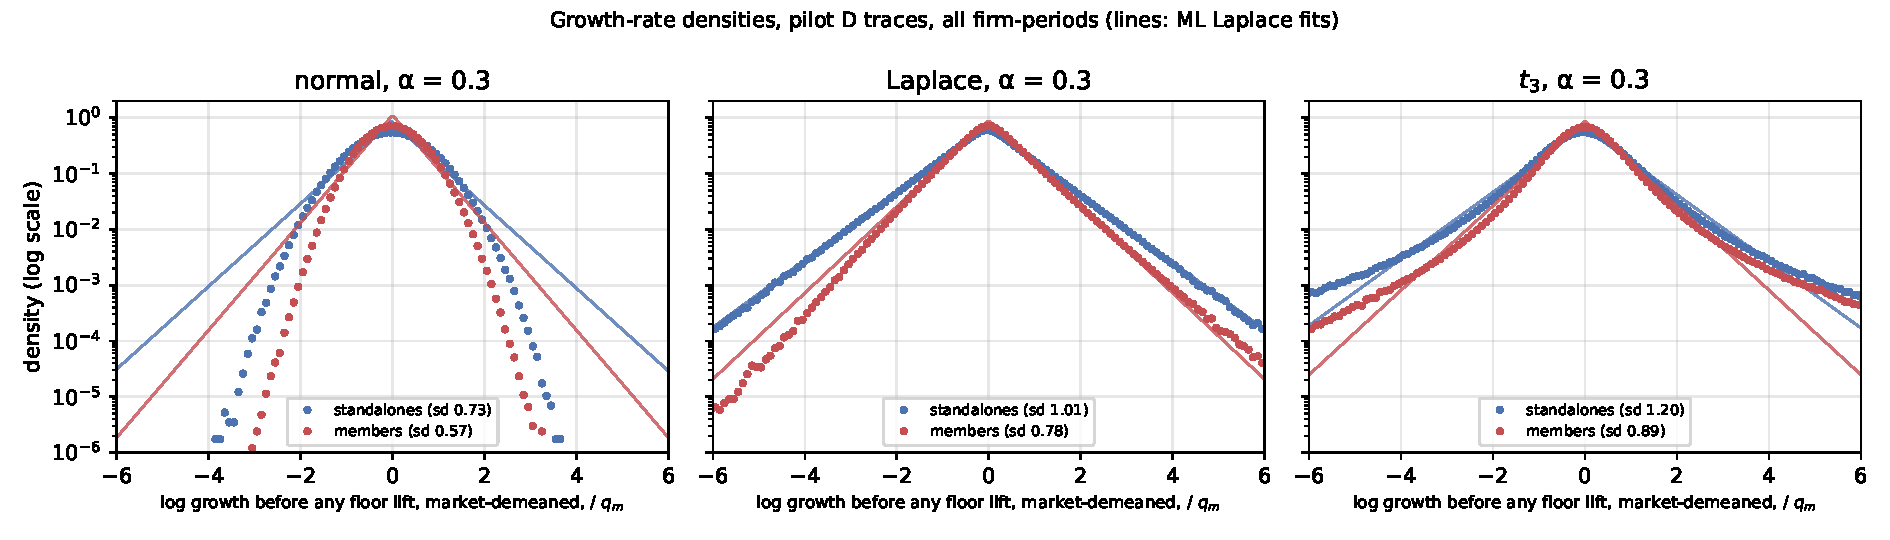
\includegraphics[width=\linewidth]{figures/appendix/growth_density_alpha0.3.pdf}
\caption{Densities of normalized per-period growth rates of members and standalones at $\alpha = 0.3$, log axis, with maximum-likelihood Laplace fits; one panel per family. 27 traced runs, moment rule.}
\label{fig:growth_density}
\end{figure}

\subsection{Concentration and rank mobility}\label{app:A17}

Table~\ref{tab:a18_concentration} gives the concentration measures behind Section~\ref{sec:results-distribution}. Within markets firms become more equal: the within-market Herfindahl index falls from 0.175--0.20 at $\alpha = 0$ to 0.14--0.17 at $\alpha = 0.3$ and 0.11--0.14 at $\alpha = 0.5$. Across the economy the units that own them become fewer and larger: the capital held by the largest ten per cent of owners, a conglomerate counted as one owner, goes from 0.65 to 0.65 (normal, with 0.67 at $\alpha = 0.3$), 0.66 to 0.74 (Laplace) and 0.68 to 0.79 ($t_3$) between $\alpha = 0$ and $0.5$; beyond $0.5$ it falls to 0.53 (normal) and 0.67 (Laplace) at $\alpha = 0.9$ while $t_3$ reaches 0.81, as the units' members grow more equal in size ($K_{\text{eff}}/K$ rises again to 0.68--0.71). Units sort by volatility and grow unequal: assortativity, the dispersion of members' market volatilities relative to that of a random set of the same size, falls from 0.60--0.61 at $\alpha = 0.01$ to 0.35--0.36 at $\alpha = 0.5$, because the consent test selects partners whose fluctuations are worth sharing from both sides; the effective number of members falls from 0.83--0.88 of $K$ to 0.64--0.68 over the same range as units accumulate a few large members and many recruits from the floor.

Tables~\ref{tab:a17_rank_mobility} and \ref{tab:a17b_rank_mobility_status} measure rank mobility from the 27 traced runs and nine traced $\alpha = 0$ runs: within each market, ranks of log share at an origin every 100 periods and 100 periods later, giving the Spearman correlation, the persistence of the top and bottom decile, leader turnover and the mean absolute rank change; a hit-free sample drops firms lifted at the floor in between and re-ranks the rest; the same by status at the origin; and the same for owning units across the economy. Pooling lowers rank mobility within markets in every family (lag-100 Spearman 0.16--0.33 at $\alpha = 0$ against 0.25--0.45 at $\alpha = 0.3$; top-decile persistence 0.31--0.48 against 0.36--0.53), partly through fewer floor lifts (0.68--0.83 of firms lifted within 100 periods against 0.52--0.71) and partly through slower movement among going concerns (members' ranks move 9--20\% less than standalones'); and it makes the top decile of owners markedly more persistent (0.32--0.49 against 0.67--0.69). Mobility is high in every cell and ranks are nearly independent at lag 500. The per-firm rank range and rank standard deviation of the earlier draft, recomputed on the traces, are at their ceiling in the floored economy and move the same way.

\begin{table}[htbp]
\centering
\caption{Concentration within markets and across owners}
\label{tab:a18_concentration}
\small
\begin{tabular}{lrrrrr}
\toprule
Family & $\alpha$ & \makecell[b]{HHI within\\{}markets} & \makecell[b]{Top-decile\\{}owners' share} & $K_{\text{eff}}/K$ & Assortativity \\
\midrule
normal & 0 & 0.175 & 0.65 & -- & -- \\
 & 0.1 & 0.164 & 0.67 & 0.75 & 0.49 \\
 & 0.3 & 0.139 & 0.67 & 0.68 & 0.39 \\
 & 0.5 & 0.109 & 0.65 & 0.65 & 0.36 \\
Laplace & 0 & 0.179 & 0.66 & -- & -- \\
 & 0.1 & 0.168 & 0.72 & 0.73 & 0.49 \\
 & 0.3 & 0.144 & 0.73 & 0.68 & 0.40 \\
 & 0.5 & 0.113 & 0.74 & 0.64 & 0.35 \\
$t_3$ & 0 & 0.201 & 0.68 & -- & -- \\
 & 0.1 & 0.191 & 0.74 & 0.74 & 0.52 \\
 & 0.3 & 0.167 & 0.77 & 0.70 & 0.42 \\
 & 0.5 & 0.136 & 0.79 & 0.67 & 0.35 \\
\bottomrule
\end{tabular}
\end{table}

\begin{sidewaystable}[htbp]
\centering
\caption{Rank mobility within markets and persistence of owners, lag 100 periods}
\label{tab:a17_rank_mobility}
\small
\begin{tabular}{lrrrrrrrr}
\toprule
Family & $\alpha$ & \makecell[b]{Spearman\\{}(all /\\{}hit-free)} & \makecell[b]{Top-decile\\{}persistence\\{}(all / hit-free)} & \makecell[b]{Leader\\{}turnover\\{}(all / hit-free)} & \makecell[b]{Mean\\{}rank\\{}change} & \makecell[b]{Share\\{}lifted\\{}within 100} & \makecell[b]{Owners:\\{}Spearman} & \makecell[b]{Owners:\\{}top-decile\\{}persistence} \\
\midrule
normal & 0 & 0.33 / 0.41 & 0.48 / 0.45 & 0.60 / 0.62 & 13.1 & 0.68 & 0.33 & 0.49 \\
 & 0.05 & 0.34 / 0.42 & 0.48 / 0.46 & 0.59 / 0.62 & 12.9 & 0.66 & 0.38 & 0.63 \\
 & 0.1 & 0.36 / 0.43 & 0.49 / 0.47 & 0.59 / 0.62 & 12.7 & 0.63 & 0.38 & 0.66 \\
 & 0.3 & 0.45 / 0.49 & 0.53 / 0.50 & 0.58 / 0.59 & 11.6 & 0.52 & 0.40 & 0.69 \\
Laplace & 0 & 0.21 / 0.31 & 0.35 / 0.36 & 0.73 / 0.71 & 14.4 & 0.78 & 0.20 & 0.37 \\
 & 0.05 & 0.22 / 0.31 & 0.36 / 0.35 & 0.73 / 0.71 & 14.3 & 0.77 & 0.24 & 0.55 \\
 & 0.1 & 0.24 / 0.32 & 0.37 / 0.35 & 0.72 / 0.72 & 14.1 & 0.75 & 0.24 & 0.59 \\
 & 0.3 & 0.32 / 0.35 & 0.41 / 0.37 & 0.71 / 0.71 & 13.2 & 0.64 & 0.27 & 0.68 \\
$t_3$ & 0 & 0.16 / 0.29 & 0.31 / 0.32 & 0.77 / 0.74 & 14.9 & 0.83 & 0.16 & 0.32 \\
 & 0.05 & 0.17 / 0.29 & 0.32 / 0.32 & 0.77 / 0.74 & 14.8 & 0.81 & 0.19 & 0.50 \\
 & 0.1 & 0.19 / 0.29 & 0.32 / 0.32 & 0.77 / 0.73 & 14.7 & 0.80 & 0.19 & 0.55 \\
 & 0.3 & 0.25 / 0.32 & 0.36 / 0.36 & 0.75 / 0.72 & 13.9 & 0.71 & 0.23 & 0.67 \\
\bottomrule
\end{tabular}
\par\smallskip\begin{minipage}{0.95\linewidth}\footnotesize Pooling lowers rank mobility within markets in every family (persistence rises with the sharing rate) and makes the top decile of owners more persistent; the hit-free columns show that part, not all, of the fall is fewer recapitalizations at the floor.\end{minipage}
\end{sidewaystable}

\begin{sidewaystable}[htbp]
\centering
\caption{Rank mobility by status at the origin, lag 100 periods}
\label{tab:a17b_rank_mobility_status}
\small
\begin{tabular}{lrrrrr}
\toprule
Family & $\alpha$ & \makecell[b]{Top-decile persistence\\{}(member / standalone)} & \makecell[b]{Mean rank change\\{}(member / standalone)} & \makecell[b]{Share lifted within 100\\{}(member / standalone)} & \makecell[b]{Members' share\\{}of the top decile} \\
\midrule
normal & 0.05 & 0.46 / 0.65 & 12.2 / 14.0 & 0.55 / 0.83 & 0.87 \\
 & 0.1 & 0.48 / 0.63 & 12.0 / 14.1 & 0.52 / 0.84 & 0.94 \\
 & 0.3 & 0.53 / 0.48 & 10.9 / 13.6 & 0.41 / 0.82 & 0.99 \\
Laplace & 0.05 & 0.35 / 0.43 & 13.6 / 15.1 & 0.67 / 0.88 & 0.88 \\
 & 0.1 & 0.37 / 0.36 & 13.4 / 15.1 & 0.65 / 0.89 & 0.93 \\
 & 0.3 & 0.41 / 0.30 & 12.5 / 14.9 & 0.54 / 0.87 & 0.97 \\
$t_3$ & 0.05 & 0.31 / 0.34 & 14.2 / 15.5 & 0.73 / 0.90 & 0.84 \\
 & 0.1 & 0.33 / 0.29 & 14.0 / 15.6 & 0.70 / 0.91 & 0.89 \\
 & 0.3 & 0.37 / 0.28 & 13.1 / 15.3 & 0.60 / 0.89 & 0.95 \\
\bottomrule
\end{tabular}
\par\smallskip\begin{minipage}{0.95\linewidth}\footnotesize Members' ranks move less than standalones' in every cell; the standalone top-decile figures rest on few firms, since members hold 84--99\% of the top decile.\end{minipage}
\end{sidewaystable}


\subsection{Scope without consent: the accept rule}\label{app:accept}

Under the accept rule every feasible proposal merges and no one leaves by choice; everything else is unchanged. It is a control without knowledge, not a behavioural alternative: it shows the scope the floor and the one-firm-per-market constraint alone permit. Table~\ref{tab:a19_accept} sets it beside the moment and loggain rules on the main power-law cells (45 runs on the main cells' seeds): $K_{\text{accept}}$ is 12.4--28.2 against 3.5--7.7, above the equal-members reference in every normal and Laplace cell and below it under $t_3$ (0.3--0.6 of $K^*$). The extra mergers are solo entries of floor-sized firms into existing units (86--89\% of the control's entries are at the floor); unit--unit mergers do not rise with consent off, because consolidated units occupy most markets and clash. The pooled share rises by 0.02--0.11, the Hill exponent by 0.00--0.04, the within-market Herfindahl index falls by 0.004--0.012, and the members' floor-hit rate rises slightly. Table~\ref{tab:decomposition-accept} is the four-part re-cut of Table~\ref{tab:decomposition} that separates what the environment permits from what consent withholds.

\begin{sidewaystable}[htbp]
\centering
\caption{The accept rule against the moment and loggain rules}
\label{tab:a19_accept}
\small
\begin{tabular}{lrrrrrrrrrr}
\toprule
Family & $\alpha$ & \makecell[b]{K:\\{}accept} & moment & loggain & \makecell[b]{Pooled:\\{}accept} & moment & \makecell[b]{Hill:\\{}accept} & moment & \makecell[b]{HHI within:\\{}accept} & moment \\
\midrule
normal & 0.1 & 17.6 & 3.7 & 3.0 & 0.95 & 0.85 & 1.12 & 1.11 & 0.160 & 0.164 \\
 & 0.3 & 22.2 & 5.5 & 4.3 & 0.97 & 0.94 & 1.21 & 1.21 & 0.133 & 0.139 \\
 & 0.5 & 28.2 & 7.7 & 6.3 & 0.98 & 0.96 & 1.37 & 1.34 & 0.106 & 0.109 \\
Laplace & 0.1 & 13.8 & 3.7 & 3.0 & 0.93 & 0.85 & 1.11 & 1.11 & 0.164 & 0.168 \\
 & 0.3 & 18.1 & 5.4 & 4.0 & 0.95 & 0.91 & 1.23 & 1.19 & 0.135 & 0.144 \\
 & 0.5 & 24.3 & 7.8 & 5.9 & 0.97 & 0.93 & 1.35 & 1.34 & 0.109 & 0.113 \\
$t_3$ & 0.1 & 12.4 & 3.5 & 2.9 & 0.91 & 0.83 & 1.04 & 1.03 & 0.188 & 0.191 \\
 & 0.3 & 16.2 & 4.8 & 3.7 & 0.94 & 0.90 & 1.13 & 1.12 & 0.160 & 0.167 \\
 & 0.5 & 21.8 & 6.8 & 5.1 & 0.96 & 0.92 & 1.26 & 1.22 & 0.127 & 0.136 \\
\bottomrule
\end{tabular}
\end{sidewaystable}

\begin{sidewaystable}[htbp]
\centering
\caption{Four-part decomposition of the distance to the equal-members reference, power-law cost; medians over five replications}
\label{tab:decomposition-accept}
\small
\begin{tabular}{lrrrrrrrrrr}
\toprule
Family & $\alpha$ & $K^*$ & $K_{\text{accept}}$ & $K_{\text{hom}}$ & $K$ & $K_{\text{loggain}}$ & Environment & Consent & Transfer & Verifiability \\
\midrule
normal & 0.1 & 8 & 17.6 & 3.8 & 3.7 & 3.0 & -9.6 (-194\%) & 13.8 (279\%) & 0.1 (2\%) & 0.6 (13\%) \\
 & 0.3 & 12 & 22.2 & 5.6 & 5.5 & 4.3 & -10.2 (-133\%) & 16.7 (216\%) & 0.1 (1\%) & 1.2 (15\%) \\
 & 0.5 & 13 & 28.2 & 8.0 & 7.7 & 6.3 & -15.2 (-228\%) & 20.2 (304\%) & 0.3 (4\%) & 1.4 (20\%) \\
\midrule
Laplace & 0.1 & 10 & 13.8 & 3.8 & 3.7 & 3.0 & -3.8 (-55\%) & 10.0 (143\%) & 0.1 (1\%) & 0.7 (10\%) \\
 & 0.3 & 16 & 18.1 & 5.5 & 5.4 & 4.0 & -2.1 (-18\%) & 12.6 (105\%) & 0.1 (1\%) & 1.4 (12\%) \\
 & 0.5 & 20 & 24.3 & 8.2 & 7.8 & 5.9 & -4.3 (-31\%) & 16.1 (115\%) & 0.4 (3\%) & 1.8 (13\%) \\
\midrule
$t_3$ & 0.1 & 20 & 12.4 & 3.5 & 3.5 & 2.9 & 7.6 (44\%) & 8.9 (52\%) & 0.0 (0\%) & 0.6 (4\%) \\
 & 0.3 & 47 & 16.2 & 4.9 & 4.8 & 3.7 & 30.8 (71\%) & 11.3 (26\%) & 0.1 (0\%) & 1.2 (3\%) \\
 & 0.5 & 50 & 21.8 & 7.0 & 6.8 & 5.1 & 28.2 (63\%) & 14.8 (33\%) & 0.2 (0\%) & 1.7 (4\%) \\
\bottomrule
\end{tabular}
\par\smallskip\begin{minipage}{0.95\linewidth}\footnotesize Environment $= K^* - K_{\text{accept}}$, consent $= K_{\text{accept}} - K_{\text{hom}}$, transfer $= K_{\text{hom}} - K$, verifiability $= K - K_{\text{loggain}}$; shares in parentheses are of $K^* - K_{\text{loggain}}$ (the four parts sum to it). $K_{\text{accept}}$: heterogeneous economy, every feasible proposal accepted and no voluntary exit (a control without knowledge). A negative environment part means the environment alone permits units larger than $K^*$. The consent part compares the heterogeneous accept economy with the homogeneous moment economy, so it also holds the homogeneous-heterogeneous difference of the accept rule.\end{minipage}
\end{sidewaystable}


\subsection{The sharing rate}\label{app:alpha}

Table~\ref{tab:endogenous} gives the endogenous-$\alpha$ block under the power-law cost and Table~\ref{tab:a13_endogenous} under all four cost forms and both rules. Units that choose their rate reach 14--18 mean members under the power-law cost, with 95--98\% of capital pooled and a tail exponent of 1.8--2.1. This is the scope that a rate near 0.9 implies, not a separate effect: along the fixed-rate grid $K$ rises from 5.4 at $\alpha = 0.3$ to 7.8 at $0.5$, and the fixed $\alpha = 0.9$ cell reproduces the endogenous block (Table~\ref{tab:robustness-b}). The ordering across families is the same as elsewhere: the heaviest tails choose a slightly lower rate and reach a smaller scope. The exponential-cost cells reach $K = 16$--23 at a lower pooled share (81--92\%). Neither heterogeneity among members nor the volatility of their markets drives the choice: across 7,630 units active at the end of a run, the Spearman correlation of a unit's time-averaged rate with the dispersion of its members' volatilities is $-0.14$ to $0.00$, and with their mean volatility 0.04--0.10. Under the loggain rule the latter was 0.14--0.26: units in more volatile markets pooled more, not because the optimum differed, it is full pooling at every volatility level, but because only there was the gain from a higher rate large enough to show through the window's noise.

\begin{table}[htbp]
\centering
\caption{The sharing rate units choose}
\label{tab:endogenous}
\small
\begin{tabular}{lrrrrrrr}
\toprule
Family & $\bar\alpha$ & median & share at 1 & $K$ & Pooled & Hill & $\rho(\alpha, \bar q)$ \\
\midrule
normal & 0.93 & 0.90 & 0.22 & 16.9 & 0.98 & 2.05 & 0.10 \\
Laplace & 0.92 & 0.90 & 0.14 & 18.0 & 0.97 & 2.07 & 0.05 \\
$t_3$ & 0.91 & 0.90 & 0.12 & 14.3 & 0.95 & 1.83 & 0.04 \\
\bottomrule
\end{tabular}
\par\smallskip\begin{minipage}{0.95\linewidth}\footnotesize Endogenous-$\alpha$ block, power-law cost, start $\alpha_C = 0.1$; adopted $\alpha$ over unit-periods; share at 1: unit-periods at $\alpha_C = 1$. $\rho$: Spearman correlation of a unit's time-averaged rate with the mean IQR of its members' markets, over the 2,468 / 2,319 / 2,843 units alive at $T$ (normal / Laplace / $t_3$). For comparison, the fixed $\alpha = 0.9$ cell gives $K = 16.0$, Hill 1.98; $K = 17.2$, Hill 1.94; $K = 13.9$, Hill 1.78 (same order).\end{minipage}
\end{table}

\begin{sidewaystable}[htbp]
\centering
\caption{Endogenous $\alpha$ by cost form}
\label{tab:a13_endogenous}
\small
\begin{tabular}{lrrrrrrr}
\toprule
Family & Cost form & $\bar\alpha$ & \makecell[b]{median,\\{}moment / loggain} & \makecell[b]{share\\{}at 1} & \makecell[b]{K,\\{}moment / loggain} & Pooled & Hill \\
\midrule
normal & power law & 0.93 & 0.90 / 0.85 & 0.22 & 16.9 / 12.1 & 0.98 & 2.05 \\
 & linear & 0.93 & 0.90 / 0.85 & 0.23 & 17.2 / 11.8 & 0.98 & 2.07 \\
 & quadratic & 0.93 & 0.90 / 0.85 & 0.20 & 17.5 / 12.6 & 0.98 & 2.02 \\
 & exponential & 0.94 & 0.95 / 0.80 & 0.24 & 23.2 / 20.5 & 0.81 & 1.88 \\
Laplace & power law & 0.92 & 0.90 / 0.80 & 0.14 & 18.0 / 11.5 & 0.97 & 2.07 \\
 & linear & 0.92 & 0.90 / 0.85 & 0.13 & 18.5 / 11.8 & 0.97 & 2.06 \\
 & quadratic & 0.93 & 0.90 / 0.80 & 0.17 & 18.8 / 12.4 & 0.97 & 2.06 \\
 & exponential & 0.93 & 0.95 / 0.85 & 0.16 & 22.1 / 16.0 & 0.91 & 2.00 \\
$t_3$ & power law & 0.91 & 0.90 / 0.80 & 0.12 & 14.3 / 8.8 & 0.95 & 1.83 \\
 & linear & 0.92 & 0.90 / 0.80 & 0.14 & 14.3 / 8.7 & 0.95 & 1.84 \\
 & quadratic & 0.91 & 0.90 / 0.80 & 0.11 & 14.4 / 9.2 & 0.95 & 1.84 \\
 & exponential & 0.91 & 0.90 / 0.80 & 0.10 & 16.0 / 10.4 & 0.92 & 1.83 \\
\bottomrule
\end{tabular}
\end{sidewaystable}


\section{Robustness}\label{app:robustness}

\subsection{Summary}

Tables~\ref{tab:robustness} and \ref{tab:robustness-b} summarize every block at $\alpha = 0.3$ (the endogenous-$\alpha$ block at its adopted rate) against the Laplace power-law baseline. The rest of this section gives each block in full.

\begin{table}[htbp]
\centering
\caption{Robustness: environment and decision parameters}
\label{tab:robustness}
\small
\begin{tabular}{llrrrr}
\toprule
Block & Variant & $K$ & Pooled & Hill & Floor exits \\
\midrule
cost form & linear & 5.2 & 0.91 & 1.18 & 35 \\
 & quadratic & 5.9 & 0.92 & 1.19 & 36 \\
 & exponential & 6.1 & 0.88 & 1.21 & 36 \\
\midrule
cost level & $\times 0.5$ & 6.0 & 0.92 & 1.20 & 35 \\
 & $\times 2$ & 4.7 & 0.91 & 1.19 & 35 \\
 & $\times 5$ & 3.9 & 0.87 & 1.17 & 33 \\
 & $\times 10$ & 3.3 & 0.79 & 1.15 & 33 \\
 & $\times 20$ & 2.8 & 0.67 & 1.13 & 33 \\
\midrule
window $l$ & 20 & 4.8 & 0.91 & 1.19 & 35 \\
 & 100 & 5.8 & 0.92 & 1.20 & 37 \\
 & 200 & 6.1 & 0.93 & 1.21 & 34 \\
 & 500 & 6.6 & 0.92 & 1.20 & 38 \\
\midrule
search $p$ & 0.2 & 6.8 & 0.97 & 1.18 & 62 \\
 & 1 & 8.0 & 0.98 & 1.18 & 116 \\
\midrule
correlation & cross-market 0.3 & 5.3 & 0.91 & 1.21 & 36 \\
\midrule
floor $c$ & 0.10 & 5.6 & 0.93 & 1.13 & 32 \\
 & 0.35 & 4.4 & 0.74 & 1.66 & 60 \\
\midrule
economy size $(M, N)$ & (25, 25) & 5.6 & 0.96 & 1.22 & 7 \\
 & (100, 25) & 6.2 & 0.96 & 1.24 & 23 \\
 & (25, 100) & 4.7 & 0.88 & 1.16 & 44 \\
 & (100, 100) & 5.2 & 0.89 & 1.17 & 170 \\
\bottomrule
\end{tabular}
\par\smallskip\begin{minipage}{0.95\linewidth}\footnotesize At $\alpha = 0.3$, Laplace shocks, power-law cost unless stated, moment rule; medians over five replications. Baseline: $K = 5.4$, pooled 0.91, Hill 1.19, 36 floor exits per period. \end{minipage}
\end{table}

\begin{table}[htbp]
\centering
\caption{Robustness: contract, shock family and decision rule}
\label{tab:robustness-b}
\small
\begin{tabular}{llrrrr}
\toprule
Block & Variant & $K$ & Pooled & Hill & Floor exits \\
\midrule
equal split (normal) & linear & 2.9 & 0.29 & 1.12 & 21 \\
 & quadratic & 3.0 & 0.33 & 1.14 & 24 \\
 & exponential & 2.8 & 0.24 & 1.09 & 21 \\
 & power law & 3.0 & 0.33 & 1.13 & 24 \\
\midrule
endogenous $\alpha$ & normal & 16.9 & 0.98 & 2.05 & 2 \\
 & Laplace & 18.0 & 0.97 & 2.07 & 4 \\
 & $t_3$ & 14.3 & 0.95 & 1.83 & 11 \\
\midrule
fixed $\alpha = 0.9$ & normal & 16.0 & 0.98 & 1.98 & 2 \\
 & Laplace & 17.2 & 0.97 & 1.94 & 5 \\
 & $t_3$ & 13.9 & 0.95 & 1.78 & 11 \\
\midrule
tail weight $\nu$ (Student-$t$) & 2.5 & 4.1 & 0.85 & 1.02 & 54 \\
 & 3 & 4.8 & 0.90 & 1.12 & 42 \\
 & 4 & 5.3 & 0.92 & 1.17 & 33 \\
\midrule
homogeneous markets & normal & 5.6 & 0.94 & 1.20 & 22 \\
 & Laplace & 5.5 & 0.91 & 1.19 & 34 \\
 & $t_3$ & 4.9 & 0.89 & 1.10 & 42 \\
\midrule
loggain rule & normal & 4.3 & 0.73 & 1.17 & 26 \\
 & Laplace & 4.0 & 0.78 & 1.16 & 37 \\
 & $t_3$ & 3.7 & 0.77 & 1.10 & 43 \\
\bottomrule
\end{tabular}
\par\smallskip\begin{minipage}{0.95\linewidth}\footnotesize Conventions as in Table~\ref{tab:robustness}; family rows are at $\alpha = 0.3$ except the endogenous-$\alpha$ block. Homogeneous markets: every market at $q = 0.20$.\end{minipage}
\end{table}


\subsection{Cost form and level}\label{app:cost}

Table~\ref{tab:a10_cost_forms} gives the four cost forms at equal $\Phi(40)$ for all three families; the form moves scope by under one member. Table~\ref{tab:costlevel} runs the power-law level from $\times 0.5$ to $\times 20$ at $\alpha = 0.3$ under both rules with the equal-members reference recomputed at each level: scope falls by about 0.6 members per doubling of the cost and the ratio $K/K^*$ rises, but the reference is never reached, because the reference falls with the cost as well. Table~\ref{tab:a10b_cost_levels} gives the $\times 0.5$ and $\times 2$ cells for every form, with $b_0$ alone scaled (power law and exponential: the whole schedule) or all coefficients scaled (linear, quadratic).

\begin{table}[htbp]
\centering
\caption{Cost forms at equal $\Phi$(40), $\alpha$ = 0.3}
\label{tab:a10_cost_forms}
\small
\begin{tabular}{lrrrrr}
\toprule
Family & Cost form & K & Pooled & Hill & Acceptance \\
\midrule
normal & power law & 5.5 & 0.94 & 1.21 & 0.29 \\
normal & linear & 5.3 & 0.93 & 1.21 & 0.26 \\
normal & quadratic & 6.4 & 0.94 & 1.22 & 0.34 \\
normal & exponential & 6.6 & 0.87 & 1.22 & 0.35 \\
Laplace & power law & 5.4 & 0.91 & 1.19 & 0.40 \\
Laplace & linear & 5.2 & 0.91 & 1.18 & 0.39 \\
Laplace & quadratic & 5.9 & 0.92 & 1.19 & 0.42 \\
Laplace & exponential & 6.1 & 0.88 & 1.21 & 0.44 \\
$t_3$ & power law & 4.8 & 0.90 & 1.12 & 0.44 \\
$t_3$ & linear & 4.6 & 0.88 & 1.10 & 0.46 \\
$t_3$ & quadratic & 4.9 & 0.88 & 1.09 & 0.49 \\
$t_3$ & exponential & 5.2 & 0.86 & 1.11 & 0.47 \\
\bottomrule
\end{tabular}
\end{table}

\begin{table}[htbp]
\centering
\caption{Cost level, power-law form, $\alpha = 0.3$; medians over five replications}
\label{tab:costlevel}
\small
\begin{tabular}{lrrrrrrrr}
\toprule
Family & Cost level & $K$ & $K$, loggain & $K^*$ & $K/K^*$ & Pooled & Accept. & Hill \\
\midrule
Laplace & 0.5 & 6.0 & 4.3 & -- & -- & 0.92 & 0.42 & 1.20 \\
 & 1 & 5.4 & 4.0 & 16 & 0.34 & 0.91 & 0.40 & 1.19 \\
 & 2 & 4.7 & 3.7 & -- & -- & 0.91 & 0.36 & 1.19 \\
 & 5 & 3.9 & 3.1 & 8 & 0.49 & 0.87 & 0.31 & 1.17 \\
 & 10 & 3.3 & 2.8 & 6 & 0.55 & 0.79 & 0.29 & 1.15 \\
 & 20 & 2.8 & 2.5 & 4 & 0.70 & 0.67 & 0.29 & 1.13 \\
\midrule
$t_3$ & 1 & 4.8 & 3.7 & 47 & 0.10 & 0.90 & 0.44 & 1.12 \\
 & 5 & 3.7 & 3.0 & 10 & 0.37 & 0.85 & 0.38 & 1.10 \\
 & 10 & 3.3 & 2.8 & 7 & 0.47 & 0.80 & 0.37 & 1.07 \\
 & 20 & 2.8 & 2.5 & 5 & 0.57 & 0.70 & 0.36 & 1.05 \\
\bottomrule
\end{tabular}
\end{table}

\begin{table}[htbp]
\centering
\caption{Cost level $\times$0.5 and $\times$2, Laplace}
\label{tab:a10b_cost_levels}
\small
\begin{tabular}{lrrrrrr}
\toprule
Scaled & Cost form & Level & $\alpha$ & K & Pooled & Acceptance \\
\midrule
$b_0$ only & exponential & $\times$0.5 & 0.1 & 4.5 & 0.75 & 0.46 \\
$b_0$ only & exponential & $\times$0.5 & 0.3 & 6.4 & 0.91 & 0.46 \\
$b_0$ only & exponential & $\times$0.5 & 0.5 & 9.5 & 0.94 & 0.44 \\
$b_0$ only & exponential & $\times$2 & 0.1 & 3.6 & 0.38 & 0.32 \\
$b_0$ only & exponential & $\times$2 & 0.3 & 5.5 & 0.81 & 0.42 \\
$b_0$ only & exponential & $\times$2 & 0.5 & 8.0 & 0.91 & 0.40 \\
$b_0$ only & linear & $\times$0.5 & 0.1 & 3.6 & 0.82 & 0.42 \\
$b_0$ only & linear & $\times$0.5 & 0.3 & 5.3 & 0.91 & 0.39 \\
$b_0$ only & linear & $\times$0.5 & 0.5 & 7.7 & 0.94 & 0.37 \\
$b_0$ only & linear & $\times$2 & 0.1 & 3.6 & 0.82 & 0.44 \\
$b_0$ only & linear & $\times$2 & 0.3 & 5.2 & 0.91 & 0.41 \\
$b_0$ only & linear & $\times$2 & 0.5 & 7.6 & 0.93 & 0.39 \\
$b_0$ only & power law & $\times$0.5 & 0.1 & 4.1 & 0.88 & 0.43 \\
$b_0$ only & power law & $\times$0.5 & 0.3 & 6.0 & 0.92 & 0.42 \\
$b_0$ only & power law & $\times$0.5 & 0.5 & 8.7 & 0.94 & 0.40 \\
$b_0$ only & power law & $\times$2 & 0.1 & 3.3 & 0.80 & 0.39 \\
$b_0$ only & power law & $\times$2 & 0.3 & 4.7 & 0.91 & 0.36 \\
$b_0$ only & power law & $\times$2 & 0.5 & 6.7 & 0.94 & 0.32 \\
$b_0$ only & quadratic & $\times$0.5 & 0.1 & 4.2 & 0.87 & 0.47 \\
$b_0$ only & quadratic & $\times$0.5 & 0.3 & 5.9 & 0.91 & 0.45 \\
$b_0$ only & quadratic & $\times$0.5 & 0.5 & 8.4 & 0.93 & 0.41 \\
$b_0$ only & quadratic & $\times$2 & 0.1 & 4.2 & 0.83 & 0.46 \\
$b_0$ only & quadratic & $\times$2 & 0.3 & 5.9 & 0.91 & 0.44 \\
$b_0$ only & quadratic & $\times$2 & 0.5 & 8.3 & 0.94 & 0.41 \\
all coefficients & linear & $\times$0.5 & 0.1 & 4.0 & 0.87 & 0.44 \\
all coefficients & linear & $\times$0.5 & 0.3 & 6.0 & 0.92 & 0.42 \\
all coefficients & linear & $\times$0.5 & 0.5 & 8.9 & 0.94 & 0.40 \\
all coefficients & linear & $\times$2 & 0.1 & 3.2 & 0.75 & 0.40 \\
all coefficients & linear & $\times$2 & 0.3 & 4.6 & 0.90 & 0.35 \\
all coefficients & linear & $\times$2 & 0.5 & 6.6 & 0.93 & 0.32 \\
all coefficients & quadratic & $\times$0.5 & 0.1 & 4.5 & 0.88 & 0.48 \\
all coefficients & quadratic & $\times$0.5 & 0.3 & 6.3 & 0.92 & 0.46 \\
all coefficients & quadratic & $\times$0.5 & 0.5 & 9.1 & 0.94 & 0.43 \\
all coefficients & quadratic & $\times$2 & 0.1 & 3.9 & 0.81 & 0.44 \\
all coefficients & quadratic & $\times$2 & 0.3 & 5.4 & 0.91 & 0.41 \\
all coefficients & quadratic & $\times$2 & 0.5 & 7.6 & 0.93 & 0.37 \\
\bottomrule
\end{tabular}
\end{table}


\subsection{Floor level, correlation and economy size}\label{app:environment}

Tables~\ref{tab:a11a_floor}--\ref{tab:a11c_size}, Laplace shocks and power-law cost. The floor level sets the tail exponent and little else: scope moves by $+3\%$ at $c = 0.10$ and $-19\%$ at $c = 0.35$ while the Hill exponent moves from 1.13 to 1.66 at $\alpha = 0.3$. Cross-market correlation of 0.3 leaves every outcome within 0.2 of the baseline. Economy size matters through the number of firms per market and barely through the number of markets, with the floor recalibrated to $c^*(N)$.

\begin{table}[htbp]
\centering
\caption{Floor level}
\label{tab:a11a_floor}
\small
\begin{tabular}{lrrrrrr}
\toprule
c & $\alpha$ & K & Pooled & Hill & Acceptance & \makecell[b]{Floor exits\\{}/ period} \\
\midrule
0.1 & 0.1 & 3.8 & 0.87 & 1.05 & 0.38 & 42.3 \\
0.1 & 0.3 & 5.6 & 0.93 & 1.13 & 0.36 & 31.5 \\
0.1 & 0.5 & 8.2 & 0.95 & 1.29 & 0.34 & 20.3 \\
0.35 & 0.1 & 3.3 & 0.68 & 1.55 & 0.60 & 69.9 \\
0.35 & 0.3 & 4.4 & 0.74 & 1.66 & 0.56 & 59.9 \\
0.35 & 0.5 & 5.8 & 0.78 & 1.80 & 0.53 & 47.7 \\
\bottomrule
\end{tabular}
\end{table}

\begin{table}[htbp]
\centering
\caption{Cross-market correlation 0.3}
\label{tab:a11b_correlation}
\small
\begin{tabular}{lrrrrrr}
\toprule
correlation & $\alpha$ & K & Pooled & Hill & Acceptance & \makecell[b]{Floor exits\\{}/ period} \\
\midrule
0.3 & 0.1 & 3.7 & 0.85 & 1.10 & 0.42 & 47.1 \\
0.3 & 0.3 & 5.3 & 0.91 & 1.21 & 0.40 & 36.3 \\
0.3 & 0.5 & 7.6 & 0.94 & 1.34 & 0.37 & 24.3 \\
\bottomrule
\end{tabular}
\end{table}

\begin{table}[htbp]
\centering
\caption{Economy size with $c^*$(N)}
\label{tab:a11c_size}
\small
\begin{tabular}{lrrrrrr}
\toprule
M / N & $\alpha$ & K & Pooled & Hill & Acceptance & \makecell[b]{Floor exits\\{}/ period} \\
\midrule
25 / 25 & 0.1 & 3.8 & 0.91 & 1.13 & 0.38 & 9.0 \\
25 / 25 & 0.3 & 5.6 & 0.96 & 1.22 & 0.40 & 6.5 \\
25 / 25 & 0.5 & 8.0 & 0.97 & 1.45 & 0.39 & 3.9 \\
25 / 100 & 0.1 & 3.5 & 0.81 & 1.10 & 0.52 & 53.9 \\
25 / 100 & 0.3 & 4.7 & 0.88 & 1.16 & 0.52 & 43.7 \\
25 / 100 & 0.5 & 6.3 & 0.91 & 1.26 & 0.50 & 31.1 \\
100 / 25 & 0.1 & 4.0 & 0.91 & 1.12 & 0.29 & 33.3 \\
100 / 25 & 0.3 & 6.2 & 0.96 & 1.24 & 0.24 & 23.1 \\
100 / 25 & 0.5 & 9.4 & 0.97 & 1.45 & 0.20 & 13.0 \\
100 / 100 & 0.1 & 3.6 & 0.82 & 1.09 & 0.46 & 215.9 \\
100 / 100 & 0.3 & 5.2 & 0.89 & 1.17 & 0.40 & 170.2 \\
100 / 100 & 0.5 & 7.6 & 0.91 & 1.28 & 0.35 & 118.3 \\
\bottomrule
\end{tabular}
\end{table}


\subsection{Homogeneous markets}\label{app:homogeneous}

Table~\ref{tab:a8_homogeneous}: every market at $q = 0.20$, power-law cost, both rules. The homogeneous economy is the $K_{\text{hom}}$ of Table~\ref{tab:decomposition}; it exceeds the heterogeneous base case by 0.0--0.4 members, which bounds the transfer conflict between members of unequal volatility.

\begin{table}[htbp]
\centering
\caption{Homogeneous block}
\label{tab:a8_homogeneous}
\small
\begin{tabular}{lrrrrrr}
\toprule
Family & Rule & $\alpha$ & K & Pooled & Acceptance & Hill \\
\midrule
normal & moment & 0.05 & 3.2 & 0.77 & 0.30 & 1.09 \\
normal & moment & 0.1 & 3.8 & 0.86 & 0.29 & 1.10 \\
normal & moment & 0.3 & 5.6 & 0.94 & 0.26 & 1.20 \\
normal & moment & 0.5 & 8.0 & 0.96 & 0.23 & 1.34 \\
normal & loggain & 0.05 & 2.8 & 0.49 & 0.32 & 1.07 \\
normal & loggain & 0.1 & 3.2 & 0.58 & 0.32 & 1.08 \\
normal & loggain & 0.3 & 4.6 & 0.75 & 0.26 & 1.18 \\
normal & loggain & 0.5 & 6.8 & 0.93 & 0.22 & 1.33 \\
Laplace & moment & 0.05 & 3.3 & 0.80 & 0.42 & 1.07 \\
Laplace & moment & 0.1 & 3.8 & 0.86 & 0.41 & 1.10 \\
Laplace & moment & 0.3 & 5.5 & 0.91 & 0.38 & 1.19 \\
Laplace & moment & 0.5 & 8.2 & 0.93 & 0.35 & 1.33 \\
Laplace & loggain & 0.05 & 2.8 & 0.57 & 0.42 & 1.07 \\
Laplace & loggain & 0.1 & 3.1 & 0.64 & 0.41 & 1.09 \\
Laplace & loggain & 0.3 & 4.2 & 0.80 & 0.35 & 1.17 \\
Laplace & loggain & 0.5 & 6.3 & 0.91 & 0.31 & 1.32 \\
$t_3$ & moment & 0.05 & 3.1 & 0.77 & 0.47 & 1.01 \\
$t_3$ & moment & 0.1 & 3.5 & 0.83 & 0.46 & 1.02 \\
$t_3$ & moment & 0.3 & 4.9 & 0.89 & 0.43 & 1.10 \\
$t_3$ & moment & 0.5 & 7.0 & 0.92 & 0.39 & 1.22 \\
$t_3$ & loggain & 0.05 & 2.7 & 0.57 & 0.46 & 1.00 \\
$t_3$ & loggain & 0.1 & 2.9 & 0.64 & 0.45 & 1.01 \\
$t_3$ & loggain & 0.3 & 3.8 & 0.79 & 0.40 & 1.08 \\
$t_3$ & loggain & 0.5 & 5.3 & 0.89 & 0.35 & 1.20 \\
\bottomrule
\end{tabular}
\end{table}


\subsection{Tail weight}\label{app:nu}

Table~\ref{tab:a9_nu}: Student-$t$ shocks with $\nu \in \{2.5, 3, 4\}$ at equal IQR, power-law cost, moment rule. The last two columns give the distribution of the window variance estimate relative to its population value over 200,000 i.i.d.\ 50-period windows at $q = 0.2$, and the share of windows in which it is below one half. Scope falls with tail weight while acceptance rises: under heavier tails firms are more willing to pool and less able to stay pooled, because members are recapitalized more often. Attrition, not consent, takes the scope.

\begin{sidewaystable}[htbp]
\centering
\caption{$\nu$ block}
\label{tab:a9_nu}
\small
\begin{tabular}{lrrrrrrrrr}
\toprule
$\nu$ & $\alpha$ & K & Pooled & Hill & Acceptance & \makecell[b]{Floor exits\\{}/ period} & \makecell[b]{Hazard\\{}ratio} & \makecell[b]{$\hat\sigma^2/\sigma^2$\\{}median [5\%, 95\%]} & \makecell[b]{share\\{}< $\tfrac12$} \\
\midrule
2.5 & 0.1 & 3.2 & 0.78 & 0.96 & 0.54 & 63.3 & 0.25 & 0.59 [0.29, 2.01] & 0.37 \\
 & 0.3 & 4.1 & 0.85 & 1.02 & 0.50 & 53.5 & 0.17 &  &  \\
 & 0.5 & 5.5 & 0.88 & 1.12 & 0.46 & 42.0 & 0.12 &  &  \\
3 & 0.1 & 3.5 & 0.83 & 1.03 & 0.47 & 53.1 & 0.19 & 0.77 [0.42, 1.98] & 0.13 \\
 & 0.3 & 4.8 & 0.90 & 1.12 & 0.44 & 42.5 & 0.13 &  &  \\
 & 0.5 & 6.8 & 0.92 & 1.22 & 0.41 & 31.2 & 0.08 &  &  \\
4 & 0.1 & 3.7 & 0.85 & 1.07 & 0.39 & 43.7 & 0.15 & 0.89 [0.53, 1.74] & 0.03 \\
 & 0.3 & 5.3 & 0.92 & 1.17 & 0.37 & 33.4 & 0.10 &  &  \\
 & 0.5 & 7.7 & 0.94 & 1.31 & 0.34 & 21.8 & 0.06 &  &  \\
\bottomrule
\end{tabular}
\end{sidewaystable}


\subsection{Equal sharing}\label{app:equalsplit}

Table~\ref{tab:a12_equal_split}: equal dollar splits of the net pool, normal shocks, four cost forms, with acceptance by proposal type (standalone--standalone, standalone--unit), voluntary exits, pool ruin (a unit's members capped at limited liability in a period) and the shortfall charged to the other members. Mean scope is 2.1--3.2 at every sharing rate and pooled capital never exceeds 34\%, against 3.2--7.7 and up to 96\% under proportional sharing. The reason is visible in who consents: proposals between two unaffiliated firms pass at 3--48\% under equal sharing against 95--100\% under proportional, proposals of a standalone to a unit at 6--17\% against 28--41\%. Under an equal split the larger partner subsidizes the smaller in every period in which it does better, which it expects to do half the time, and refuses. The contract decides whether conglomerates exist at all.

\begin{sidewaystable}[htbp]
\centering
\caption{Equal-split block}
\label{tab:a12_equal_split}
\small
\begin{tabular}{lrrrrrrrr}
\toprule
Cost form & $\alpha$ & K & Pooled & \makecell[b]{Acceptance\\{}s--s} & \makecell[b]{Acceptance\\{}s--u} & \makecell[b]{Voluntary\\{}exits / period} & \makecell[b]{Pool ruin\\{}/ period} & \makecell[b]{Shortfall\\{}/ period} \\
\midrule
exponential & 0.05 & 2.2 & 0.03 & 0.03 & 0.06 & 0.5 & 0.000 & 0.0e+00 \\
 & 0.1 & 2.5 & 0.14 & 0.16 & 0.13 & 2.4 & 0.001 & 7.1e-06 \\
 & 0.3 & 2.8 & 0.24 & 0.30 & 0.14 & 4.0 & 0.010 & 5.6e-04 \\
 & 0.5 & 2.9 & 0.25 & 0.29 & 0.13 & 4.7 & 0.029 & 2.5e-03 \\
linear & 0.05 & 2.5 & 0.26 & 0.39 & 0.15 & 3.3 & 0.000 & 0.0e+00 \\
 & 0.1 & 2.6 & 0.28 & 0.41 & 0.15 & 3.5 & 0.001 & 1.4e-05 \\
 & 0.3 & 2.9 & 0.29 & 0.37 & 0.14 & 4.2 & 0.012 & 7.4e-04 \\
 & 0.5 & 3.0 & 0.29 & 0.33 & 0.13 & 4.8 & 0.039 & 3.2e-03 \\
power law & 0.05 & 2.6 & 0.31 & 0.48 & 0.17 & 3.1 & 0.000 & 0.0e+00 \\
 & 0.1 & 2.7 & 0.32 & 0.48 & 0.17 & 3.3 & 0.001 & 3.3e-05 \\
 & 0.3 & 3.0 & 0.33 & 0.43 & 0.16 & 3.9 & 0.017 & 1.2e-03 \\
 & 0.5 & 3.1 & 0.33 & 0.38 & 0.14 & 4.6 & 0.050 & 3.9e-03 \\
quadratic & 0.05 & 2.7 & 0.29 & 0.45 & 0.17 & 3.2 & 0.000 & 0.0e+00 \\
 & 0.1 & 2.7 & 0.31 & 0.46 & 0.17 & 3.3 & 0.001 & 2.6e-05 \\
 & 0.3 & 3.0 & 0.33 & 0.43 & 0.16 & 4.0 & 0.016 & 8.9e-04 \\
 & 0.5 & 3.1 & 0.33 & 0.37 & 0.14 & 4.6 & 0.046 & 3.8e-03 \\
\bottomrule
\end{tabular}
\end{sidewaystable}


\section{Computation}\label{app:computation}

\subsection{Identity protocol and tests}\label{app:identity}

Every change to the code after the model was frozen (the diagnostics, the limited-liability correction, the counters, the moment rule, the production block and the traced runs) was accompanied by an identity check: every scenario whose behaviour the change should not touch is rerun on the new code and its result and summary row compared byte for byte with the stored ones, excluding runtime fields and new keys. The production block passes 1,995 of 1,995 scenarios and the accept-rule addition 2,055 of 2,055; the loggain reference block is frozen and verified by checksum. The test suite (281 tests) covers the pooling identity under limited liability (unit capital after pooling equals the sum of members' gross returns net of the coordination cost, to $10^{-9}$), the moment rule against hand-computed cases and against the loggain replay on long windows, the kernel counters' sums, the design counts and the summary schema. Three pool wipeouts (every member of a unit at the floor in the same period) occurred in 1,995 runs, one event each; they are counted, not asserted away.

\subsection{Files and provenance}\label{app:files}

The repository holds the simulation code, the design files, the per-run summaries of the production block and the loggain reference block, the traced runs' panels and every derived file behind a table or figure; \texttt{analysis/paper\_tables.py}, \texttt{analysis/paper\_figures.py} and \texttt{analysis/appendix\_tables.py} regenerate every exhibit from them. The commit the paper is frozen on and the archive DOI are given in the code and data availability statement.
